% Options for packages loaded elsewhere
\PassOptionsToPackage{unicode}{hyperref}
\PassOptionsToPackage{hyphens}{url}
%
\documentclass[
]{book}
\usepackage{amsmath,amssymb}
\usepackage{lmodern}
\usepackage{iftex}
\ifPDFTeX
  \usepackage[T1]{fontenc}
  \usepackage[utf8]{inputenc}
  \usepackage{textcomp} % provide euro and other symbols
\else % if luatex or xetex
  \usepackage{unicode-math}
  \defaultfontfeatures{Scale=MatchLowercase}
  \defaultfontfeatures[\rmfamily]{Ligatures=TeX,Scale=1}
\fi
% Use upquote if available, for straight quotes in verbatim environments
\IfFileExists{upquote.sty}{\usepackage{upquote}}{}
\IfFileExists{microtype.sty}{% use microtype if available
  \usepackage[]{microtype}
  \UseMicrotypeSet[protrusion]{basicmath} % disable protrusion for tt fonts
}{}
\makeatletter
\@ifundefined{KOMAClassName}{% if non-KOMA class
  \IfFileExists{parskip.sty}{%
    \usepackage{parskip}
  }{% else
    \setlength{\parindent}{0pt}
    \setlength{\parskip}{6pt plus 2pt minus 1pt}}
}{% if KOMA class
  \KOMAoptions{parskip=half}}
\makeatother
\usepackage{xcolor}
\usepackage{color}
\usepackage{fancyvrb}
\newcommand{\VerbBar}{|}
\newcommand{\VERB}{\Verb[commandchars=\\\{\}]}
\DefineVerbatimEnvironment{Highlighting}{Verbatim}{commandchars=\\\{\}}
% Add ',fontsize=\small' for more characters per line
\usepackage{framed}
\definecolor{shadecolor}{RGB}{248,248,248}
\newenvironment{Shaded}{\begin{snugshade}}{\end{snugshade}}
\newcommand{\AlertTok}[1]{\textcolor[rgb]{0.94,0.16,0.16}{#1}}
\newcommand{\AnnotationTok}[1]{\textcolor[rgb]{0.56,0.35,0.01}{\textbf{\textit{#1}}}}
\newcommand{\AttributeTok}[1]{\textcolor[rgb]{0.77,0.63,0.00}{#1}}
\newcommand{\BaseNTok}[1]{\textcolor[rgb]{0.00,0.00,0.81}{#1}}
\newcommand{\BuiltInTok}[1]{#1}
\newcommand{\CharTok}[1]{\textcolor[rgb]{0.31,0.60,0.02}{#1}}
\newcommand{\CommentTok}[1]{\textcolor[rgb]{0.56,0.35,0.01}{\textit{#1}}}
\newcommand{\CommentVarTok}[1]{\textcolor[rgb]{0.56,0.35,0.01}{\textbf{\textit{#1}}}}
\newcommand{\ConstantTok}[1]{\textcolor[rgb]{0.00,0.00,0.00}{#1}}
\newcommand{\ControlFlowTok}[1]{\textcolor[rgb]{0.13,0.29,0.53}{\textbf{#1}}}
\newcommand{\DataTypeTok}[1]{\textcolor[rgb]{0.13,0.29,0.53}{#1}}
\newcommand{\DecValTok}[1]{\textcolor[rgb]{0.00,0.00,0.81}{#1}}
\newcommand{\DocumentationTok}[1]{\textcolor[rgb]{0.56,0.35,0.01}{\textbf{\textit{#1}}}}
\newcommand{\ErrorTok}[1]{\textcolor[rgb]{0.64,0.00,0.00}{\textbf{#1}}}
\newcommand{\ExtensionTok}[1]{#1}
\newcommand{\FloatTok}[1]{\textcolor[rgb]{0.00,0.00,0.81}{#1}}
\newcommand{\FunctionTok}[1]{\textcolor[rgb]{0.00,0.00,0.00}{#1}}
\newcommand{\ImportTok}[1]{#1}
\newcommand{\InformationTok}[1]{\textcolor[rgb]{0.56,0.35,0.01}{\textbf{\textit{#1}}}}
\newcommand{\KeywordTok}[1]{\textcolor[rgb]{0.13,0.29,0.53}{\textbf{#1}}}
\newcommand{\NormalTok}[1]{#1}
\newcommand{\OperatorTok}[1]{\textcolor[rgb]{0.81,0.36,0.00}{\textbf{#1}}}
\newcommand{\OtherTok}[1]{\textcolor[rgb]{0.56,0.35,0.01}{#1}}
\newcommand{\PreprocessorTok}[1]{\textcolor[rgb]{0.56,0.35,0.01}{\textit{#1}}}
\newcommand{\RegionMarkerTok}[1]{#1}
\newcommand{\SpecialCharTok}[1]{\textcolor[rgb]{0.00,0.00,0.00}{#1}}
\newcommand{\SpecialStringTok}[1]{\textcolor[rgb]{0.31,0.60,0.02}{#1}}
\newcommand{\StringTok}[1]{\textcolor[rgb]{0.31,0.60,0.02}{#1}}
\newcommand{\VariableTok}[1]{\textcolor[rgb]{0.00,0.00,0.00}{#1}}
\newcommand{\VerbatimStringTok}[1]{\textcolor[rgb]{0.31,0.60,0.02}{#1}}
\newcommand{\WarningTok}[1]{\textcolor[rgb]{0.56,0.35,0.01}{\textbf{\textit{#1}}}}
\usepackage{longtable,booktabs,array}
\usepackage{calc} % for calculating minipage widths
% Correct order of tables after \paragraph or \subparagraph
\usepackage{etoolbox}
\makeatletter
\patchcmd\longtable{\par}{\if@noskipsec\mbox{}\fi\par}{}{}
\makeatother
% Allow footnotes in longtable head/foot
\IfFileExists{footnotehyper.sty}{\usepackage{footnotehyper}}{\usepackage{footnote}}
\makesavenoteenv{longtable}
\usepackage{graphicx}
\makeatletter
\def\maxwidth{\ifdim\Gin@nat@width>\linewidth\linewidth\else\Gin@nat@width\fi}
\def\maxheight{\ifdim\Gin@nat@height>\textheight\textheight\else\Gin@nat@height\fi}
\makeatother
% Scale images if necessary, so that they will not overflow the page
% margins by default, and it is still possible to overwrite the defaults
% using explicit options in \includegraphics[width, height, ...]{}
\setkeys{Gin}{width=\maxwidth,height=\maxheight,keepaspectratio}
% Set default figure placement to htbp
\makeatletter
\def\fps@figure{htbp}
\makeatother
\setlength{\emergencystretch}{3em} % prevent overfull lines
\providecommand{\tightlist}{%
  \setlength{\itemsep}{0pt}\setlength{\parskip}{0pt}}
\setcounter{secnumdepth}{5}
\usepackage{booktabs}
\ifLuaTeX
  \usepackage{selnolig}  % disable illegal ligatures
\fi
\usepackage[]{natbib}
\bibliographystyle{plainnat}
\IfFileExists{bookmark.sty}{\usepackage{bookmark}}{\usepackage{hyperref}}
\IfFileExists{xurl.sty}{\usepackage{xurl}}{} % add URL line breaks if available
\urlstyle{same} % disable monospaced font for URLs
\hypersetup{
  pdftitle={Flower photogrammetry and 3D modeling protocol},
  pdfauthor={Marion Leménager; Jérôme Burkiewicz; Daniel Schoen; Diana Constanza Diaz Cardona; Simon Joly},
  hidelinks,
  pdfcreator={LaTeX via pandoc}}

\title{Flower photogrammetry and 3D modeling protocol}
\author{Marion Leménager \and Jérôme Burkiewicz \and Daniel Schoen \and Diana Constanza Diaz Cardona \and Simon Joly}
\date{2022-09-16}

\usepackage{amsthm}
\newtheorem{theorem}{Theorem}[chapter]
\newtheorem{lemma}{Lemma}[chapter]
\newtheorem{corollary}{Corollary}[chapter]
\newtheorem{proposition}{Proposition}[chapter]
\newtheorem{conjecture}{Conjecture}[chapter]
\theoremstyle{definition}
\newtheorem{definition}{Definition}[chapter]
\theoremstyle{definition}
\newtheorem{example}{Example}[chapter]
\theoremstyle{definition}
\newtheorem{exercise}{Exercise}[chapter]
\theoremstyle{definition}
\newtheorem{hypothesis}{Hypothesis}[chapter]
\theoremstyle{remark}
\newtheorem*{remark}{Remark}
\newtheorem*{solution}{Solution}
\begin{document}
\maketitle

{
\setcounter{tocdepth}{1}
\tableofcontents
}
\hypertarget{about}{%
\chapter{About}\label{about}}

This protocol describes how to obtain three-dimensional (3D) reconstructions of flowers using photogrammetry. It describes in details the set-up, settings and steps that has worked for us for building accurate flower models, but other approaches are certainly possible. Hence, we hope this protocol serves as a starting point rather than a final protocol. We welcome any comments.

\hypertarget{disclaimer}{%
\section{Disclaimer}\label{disclaimer}}

We provide this protocol as guidelines, without any guaranty.

\hypertarget{usage}{%
\section{Usage}\label{usage}}

Each \textbf{bookdown} chapter is an .Rmd file, and each .Rmd file can contain one (and only one) chapter. A chapter \emph{must} start with a first-level heading: \texttt{\#\ A\ good\ chapter}, and can contain one (and only one) first-level heading.

Use second-level and higher headings within chapters like: \texttt{\#\#\ A\ short\ section} or \texttt{\#\#\#\ An\ even\ shorter\ section}.

The \texttt{index.Rmd} file is required, and is also your first book chapter. It will be the homepage when you render the book.

\hypertarget{render-book}{%
\section{Render book}\label{render-book}}

You can render the HTML version of this example book without changing anything:

\begin{enumerate}
\def\labelenumi{\arabic{enumi}.}
\item
  Find the \textbf{Build} pane in the RStudio IDE, and
\item
  Click on \textbf{Build Book}, then select your output format, or select ``All formats'' if you'd like to use multiple formats from the same book source files.
\end{enumerate}

Or build the book from the R console:

\begin{Shaded}
\begin{Highlighting}[]
\NormalTok{bookdown}\SpecialCharTok{::}\FunctionTok{render\_book}\NormalTok{()}
\end{Highlighting}
\end{Shaded}

To render this example to PDF as a \texttt{bookdown::pdf\_book}, you'll need to install XeLaTeX. You are recommended to install TinyTeX (which includes XeLaTeX): \url{https://yihui.org/tinytex/}.

\hypertarget{preview-book}{%
\section{Preview book}\label{preview-book}}

As you work, you may start a local server to live preview this HTML book. This preview will update as you edit the book when you save individual .Rmd files. You can start the server in a work session by using the RStudio add-in ``Preview book'', or from the R console:

\begin{Shaded}
\begin{Highlighting}[]
\NormalTok{bookdown}\SpecialCharTok{::}\FunctionTok{serve\_book}\NormalTok{()}
\end{Highlighting}
\end{Shaded}

\hypertarget{materials}{%
\chapter{Materials}\label{materials}}

\hypertarget{lighting}{%
\section{Lighting}\label{lighting}}

It is important to have good lighting conditions to take the
photographs. To optimize the lighting conditions, we use a \href{https://neewer.com/collections/shooting-tent}{Neewer
portable lighting box} to
recreate lighting studio conditions and reduce shading on the object to
a maximum. This lightbox needs to be powered from an outlet or from an
external battery. The color of the background used should contrast with
the color of the flowers to be photographed.

\hypertarget{turn-table}{%
\section{Turn table}\label{turn-table}}

We use an automated turntable and shutter release device (\href{https://www.bhphotovideo.com/c/product/1486043-REG/syrp_sykit_0043_genie_mini_ii_turntable.html/quick-compare}{Syrp Genie
mini II and
turntable})
to rotate each flower on itself (360) and trigger a predetermined number
of pictures from the camera to get pictures from all around the flower.
The genie mini II has several hours of autonomy according to its use,
but it can be plugged in a source of energy during the process (external
battery, plug, or usb). This device is easily controlled and set
remotely via its application "Syrp" (Figure
\protect\hyperlink{fig:syrp_app}{1}) on
any kind of smartphone by Bluetooth
(\href{https://apps.apple.com/us/app/syrp/id1387335063}{Appstore} or
\href{https://play.google.com/store/apps/details?id=nz.co.syrp.genie2\&hl=fr_CA\&gl=US}{Playstore})
after the device has been paired with your phone and after any updates
suggested by the device has been done.

We also use a 1cm scale placed adjacently to the flower, and include a
label describing the species name, collection number, date of
collection, location, and coordinates.

\begin{figure}
\hypertarget{fig:syrp_app}{%
\centering

\includegraphics[width=2cm,height=\textheight]{Figures/Syrp_app.png}
\caption{Syrp application}\label{fig:syrp_app}
}
\end{figure}

\hypertarget{camera}{%
\section{Camera}\label{camera}}

It is important to have very sharp pictures for optimal model
construction. However, a professional camera is not necessary. We
obtained good results with a Canon T2i/550D camera that shoots 18.0 MP
RAW photos (5184 x 3456 pixels). We recommend a fixed macro lens (we use
a 60mm fixed Canon lens). Avoid using a lens that isn't fixed : zooming
in and out can create artifacts during the model reconstruction. Ideally
the flower should take a large portion of the photographs for best
results. We also use a flexible short tripod to support the camera and
easily modify the angle at which we take each series of photos.

\hypertarget{color-chart}{%
\section{Color chart}\label{color-chart}}

To calibrate the photos for color, we use a \href{https://www.xrite.com/categories/calibration-profiling/colorchecker-classic-family/colorchecker-passport-photo-2}{Xrite ColorChecker Passport
Photo
2}.
The main target that we use is the classic target with a 24-patch color
reference target to create Digital Negative (DNG) (\citet{Adobe2012DNG}) camera
profiles from a raw photo (called DNG conversion), and the 75\% neutral
gray patch to calibrate for light exposure.

\begin{figure}
\hypertarget{fig:xrite_description}{%
\centering
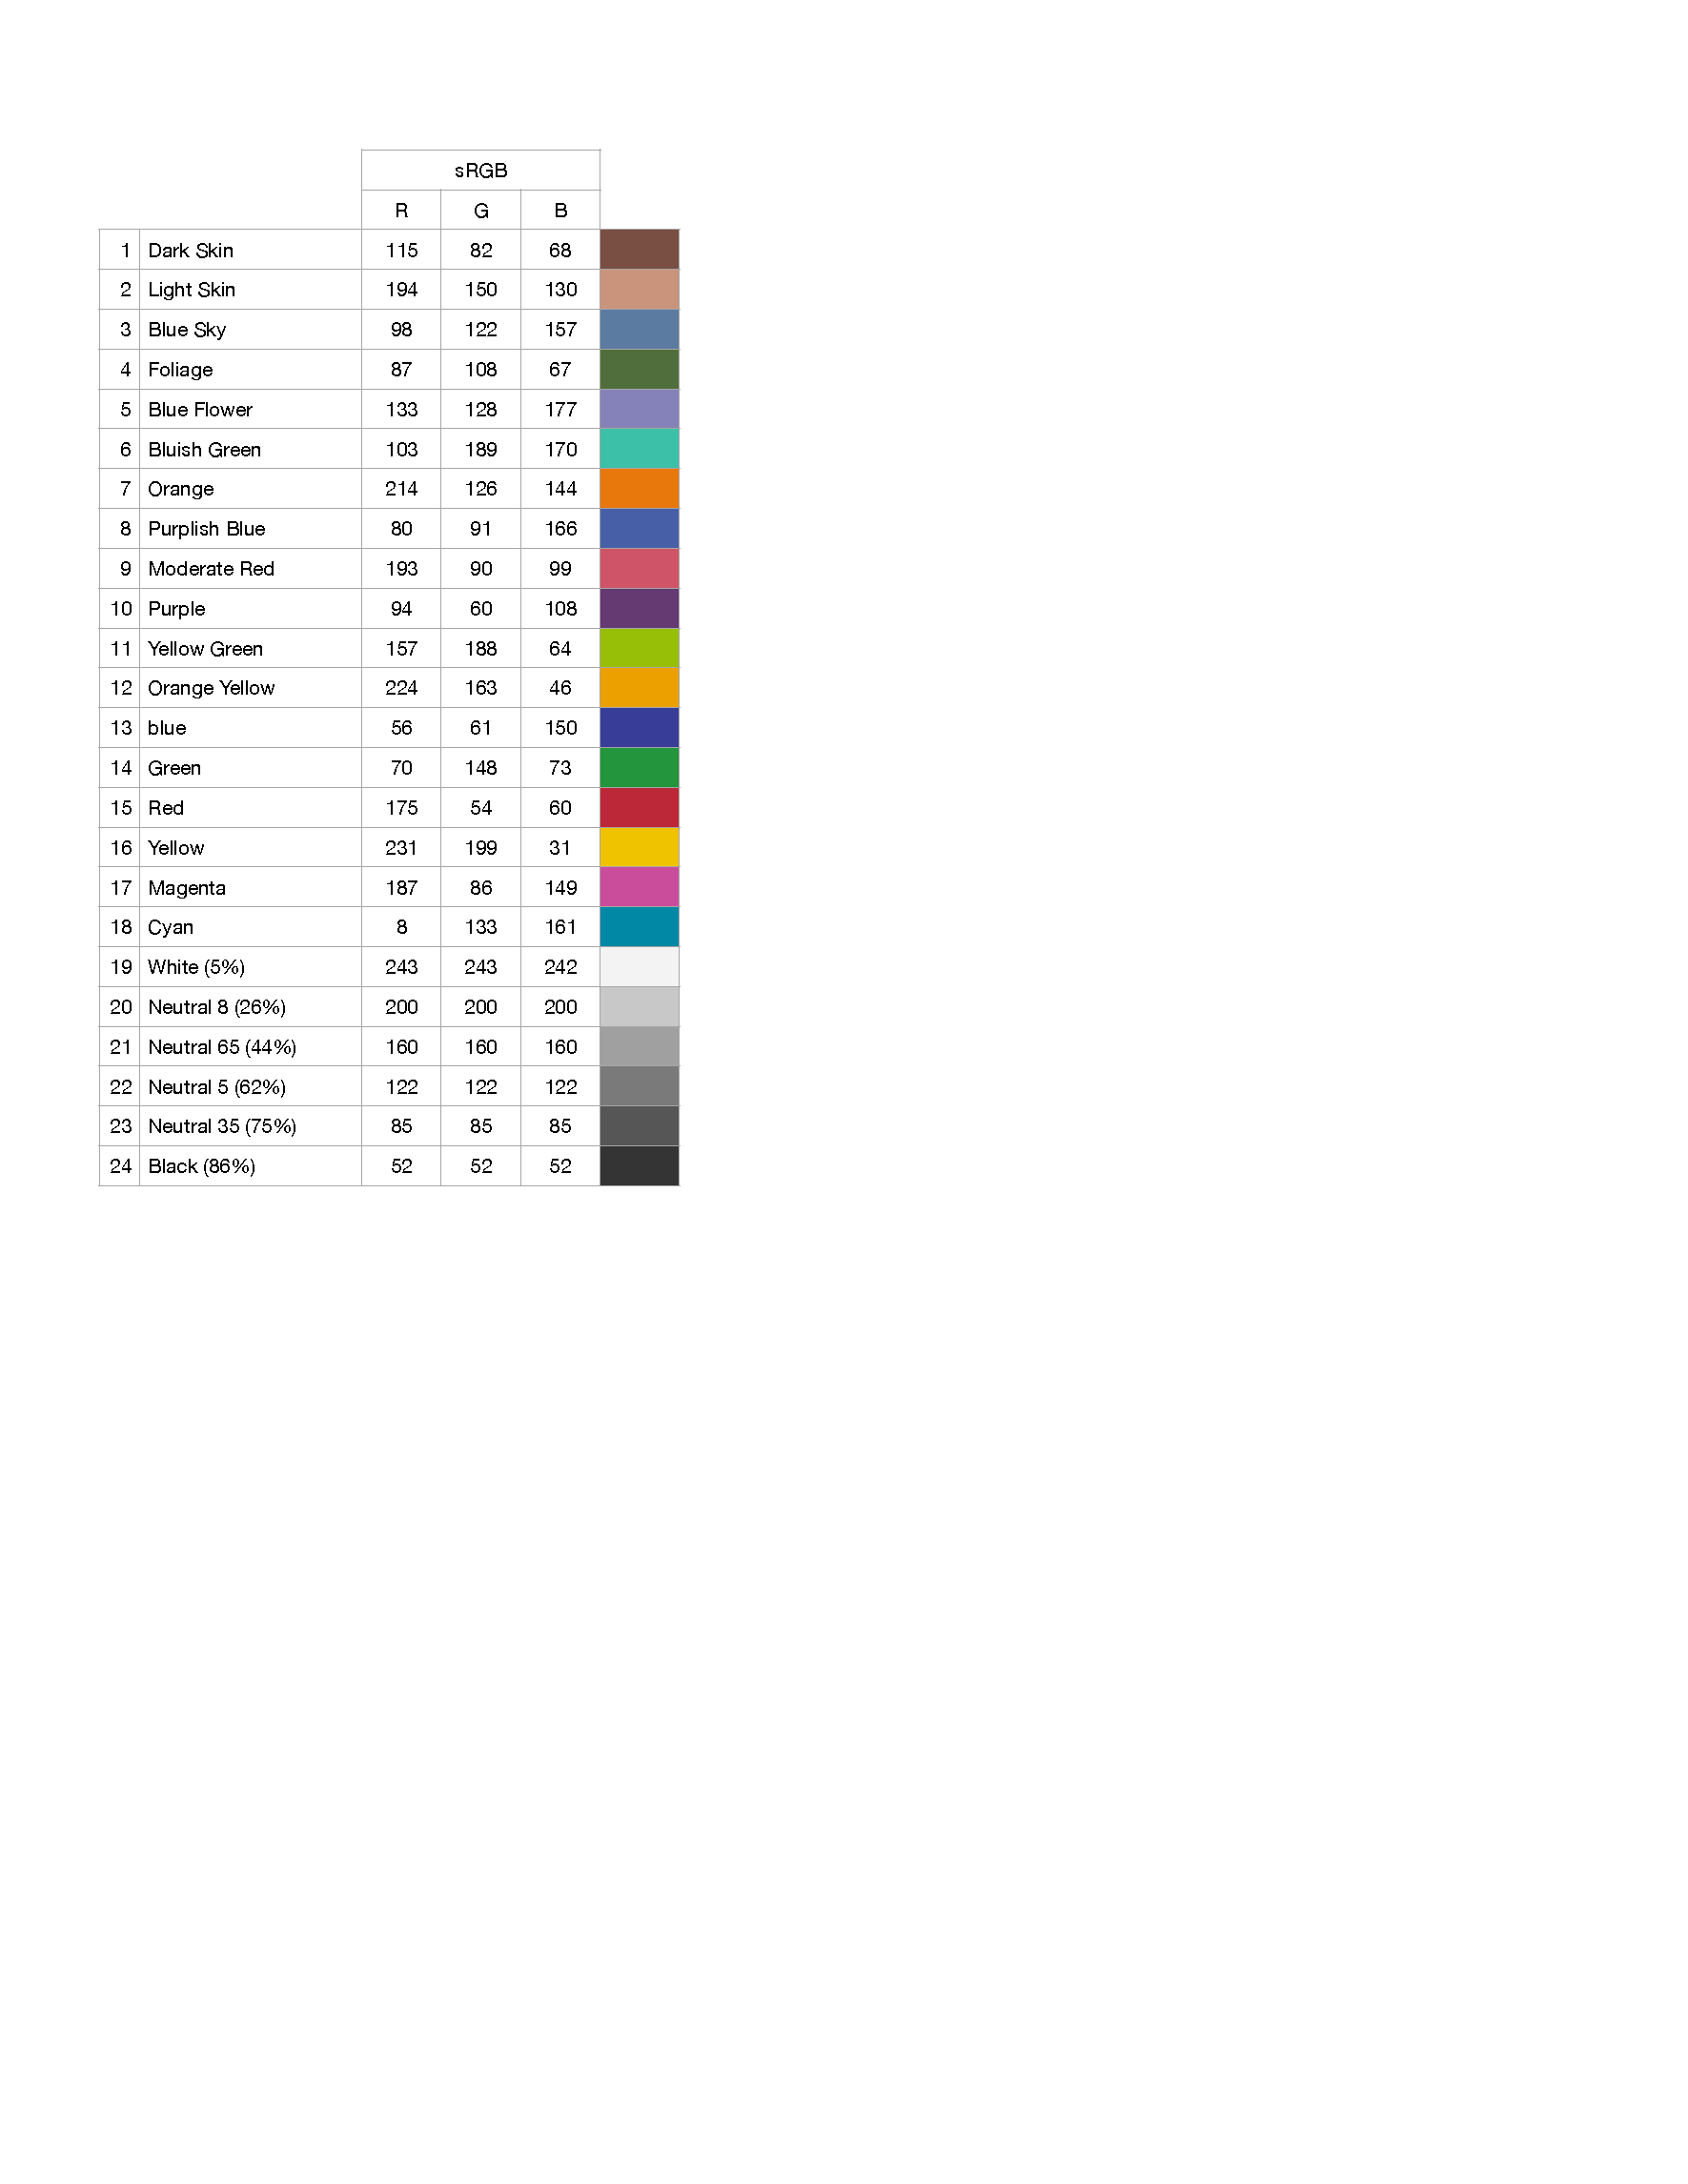
\includegraphics[width=7cm,height=\textheight]{Figures/Color chart sRGB values.pdf}
\caption{Xrite color chart details for standard Red Green and Blue (sRGB)
values. The 75\% neutral gray has values of 0.33 (85/255) for Red Green
Blue channels in the LightRoom
software.}\label{fig:xrite_description}
}
\end{figure}

\hypertarget{software}{%
\section{Software}\label{software}}

To convert RAW photos (CR2 for Canon Raw Version 2 image files) to DNG
files, we either use directly \href{https://www.adobe.com/ca_fr/products/photoshop-lightroom-classic.html}{Adobe Lightroom
Classic}
to export in DNG format the CR2 photos or \href{https://helpx.adobe.com/camera-raw/using/adobe-dng-converter.html}{Adobe DNG
converter}.
To calibrate the photos according to the color chart, we use the \href{https://xritephoto.com/ph_product_overview.aspx?ID=938\&Action=Support\&SoftwareID=2030}{Xrite
Color
Checker}
software to create DCP camera profiles from DNG files, and Adobe
Lightroom to use these profiles and apply them on an entire set of
photos that need the same calibration. To reconstruct the 3D models from
photos, we use \href{https://www.agisoft.com/downloads/installer/}{Agisoft
Metashape}.

\begin{figure}
\centering

\includegraphics[width=0.4\textwidth,height=\textheight]{Figures/logo Adobe DNG Converter.png}
\caption{Adobe DNG
Converter}
\end{figure}

\begin{figure}
\centering

\includegraphics[width=0.6\textwidth,height=\textheight]{Figures/logo ColorChecker Camera Calibration.png}
\caption{ColorChecker Camera
Calibration}
\end{figure}

\begin{figure}
\centering

\includegraphics[width=0.3\textwidth,height=\textheight]{Figures/logo Lrc.png}
\caption{Adobe Lightroom Classic}
\end{figure}

\hypertarget{flowers}{%
\section{Flowers}\label{flowers}}

Collect fresh flowers from the plant, label them and store them in a
cool place or with the tip of the peduncle in some water to prevent
accelerated wilting. Different flowers will wilt at different paces.
Flowers are pinned through the floral receptacle or peduncle using
entomological pins in dense foam at the center of the turntable.
Alternatively, flowers can be secured in a truncated pipette tip, itself
fixed on the turntable, or with alligator clips to rapidly fix the
flowers.

Store flowers in 50mL Eppendorf tubes or in foam box no more than an
hour before taking photos of them.\\
\strut \\
In some cases, it is necessary to remove sepals from the flower before
building the model to accurately study the corolla shape. To do this,
use a razor blade and mark the sepal intersections with a waterproof
pen. The marks will help for the model construction and more importantly
landmarks positioning.

\hypertarget{summary-of-materials-and-software}{%
\section{Summary of materials and software}\label{summary-of-materials-and-software}}

L5cm\textbar L9cm\textbar C1.7cm

\begin{center}\rule{0.5\linewidth}{0.5pt}\end{center}

\& \&\\

\begin{center}\rule{0.5\linewidth}{0.5pt}\end{center}

\hfill\break

\begin{center}\rule{0.5\linewidth}{0.5pt}\end{center}

Camera \& Digital Single-Lens Reflex (DSLR) (e.g.~Canon t2i) \& from
\$500\\

\begin{center}\rule{0.5\linewidth}{0.5pt}\end{center}

Macro lens \& A preferably fixed lens (e.g.~Canon 60mm f/2.8 Macro lens)
\& from \$400\\

\begin{center}\rule{0.5\linewidth}{0.5pt}\end{center}

Tripod \& Preferably flexible, such as a gorillapod \& e.g.~\$80\\

\begin{center}\rule{0.5\linewidth}{0.5pt}\end{center}

Stepping motor and turntable kit \& \href{https://www.bhphotovideo.com/c/product/1486043-REG/syrp_sykit_0043_genie_mini_ii_turntable.html/quick-compare}{Genie mini
II},
Shoot smooth rotating video and interactive 360\({^\circ}\) images of
objects. Full iOS and Android App control via Bluetooth. Battery life:
6hrs video and 15hrs time-lapse. Panning payload 8.8lbs/4kgs \& \$328.00\\

\begin{center}\rule{0.5\linewidth}{0.5pt}\end{center}

Lightbox \& A portable photo studio, e.g.
\href{https://neewer.com/products/lighting-studio-10094456?_pos=2\&_sid=bde9f6ddb\&_ss=r}{Neewer}
20"/50cm foldable portable photography lighting kit (Neewer Technology
Co.~LTD, Shenzhen, China), adjustable brightness with 120 LED lights,
CRI (colour Rendering Index) of 85+, 6000-6500K colour temperature,
needs to be powered by a portable battery in the field, white, grey, and
black backdrops. In the bracket of light intensities possible for this
lightbox, we used an intermediate light intensity. \[maximum;usually
used; minimum\] lux light intensities correspond to \[3140;2680;1330\]
lux for a white backdrop and \[330;305;238\] Lux with a black backdrop.
\& \$79.99\\

\begin{center}\rule{0.5\linewidth}{0.5pt}\end{center}

External battery \& Powering source for in-field photo capture,
essentially for the lightbox or to recharge batteries \& optional\\

\begin{center}\rule{0.5\linewidth}{0.5pt}\end{center}

\hfill\break
Flower \& Freshly cut flower with peduncle and floral receptacle \& /\\
Labels and container \& Identification and storage of fresh flowers to
avoid damage and avoid wilting \& /\\
Turntable labels \& Identification to species, collector, collection
number, date, locality, and coordinates, and the chunk number. To use as
a separate photo before each run of photos. \& /\\
Razor blade \& To remove sepals \& /\\
Small block of dense foam \& To fix flowers in place with a pin at the
center of the turntable. \& /\\
Entomological pins \& To pin through the peduncle or floral receptacle
and fix the flower on the turntable. \& /\\

\begin{center}\rule{0.5\linewidth}{0.5pt}\end{center}

Scale \& A 1 cm scale as reference \& /\\

\begin{center}\rule{0.5\linewidth}{0.5pt}\end{center}

\hfill\break

\begin{center}\rule{0.5\linewidth}{0.5pt}\end{center}

Color chart \& A color reference to calibrate RAW photos (e.g.~\href{https://www.xrite.com/categories/calibration-profiling/colorchecker-targets/colorchecker-passport-photo-2}{X-rite
ColorChecker
Passport})
\& e.g.~\$99.00\\

\begin{center}\rule{0.5\linewidth}{0.5pt}\end{center}

Color calibration software \& ColorChecker Camera Calibration, Xrite
software for automatic color profile creation \& Free\\

\begin{center}\rule{0.5\linewidth}{0.5pt}\end{center}

Photo editing software \& Adobe Photoshop Lightroom, editing software for
image color calibration in batch \& Payment plans vary\\

\begin{center}\rule{0.5\linewidth}{0.5pt}\end{center}

DNG conversion software \& Adobe DNG converter, to convert Camera Raw
files from supported cameras to the more widely used DNG raw files \&
Free\\

\begin{center}\rule{0.5\linewidth}{0.5pt}\end{center}

\hfill\break
3D reconstruction from photogrammetry software \& Agisoft Metashape Pro
Software \& \$549 Academic price\\

\begin{center}\rule{0.5\linewidth}{0.5pt}\end{center}

\hypertarget{cross}{%
\chapter{Cross-references}\label{cross}}

Cross-references make it easier for your readers to find and link to elements in your book.

\hypertarget{chapters-and-sub-chapters}{%
\section{Chapters and sub-chapters}\label{chapters-and-sub-chapters}}

There are two steps to cross-reference any heading:

\begin{enumerate}
\def\labelenumi{\arabic{enumi}.}
\tightlist
\item
  Label the heading: \texttt{\#\ Hello\ world\ \{\#nice-label\}}.

  \begin{itemize}
  \tightlist
  \item
    Leave the label off if you like the automated heading generated based on your heading title: for example, \texttt{\#\ Hello\ world} = \texttt{\#\ Hello\ world\ \{\#hello-world\}}.
  \item
    To label an un-numbered heading, use: \texttt{\#\ Hello\ world\ \{-\#nice-label\}} or \texttt{\{\#\ Hello\ world\ .unnumbered\}}.
  \end{itemize}
\item
  Next, reference the labeled heading anywhere in the text using \texttt{\textbackslash{}@ref(nice-label)}; for example, please see Chapter \ref{cross}.

  \begin{itemize}
  \tightlist
  \item
    If you prefer text as the link instead of a numbered reference use: \protect\hyperlink{cross}{any text you want can go here}.
  \end{itemize}
\end{enumerate}

\hypertarget{captioned-figures-and-tables}{%
\section{Captioned figures and tables}\label{captioned-figures-and-tables}}

Figures and tables \emph{with captions} can also be cross-referenced from elsewhere in your book using \texttt{\textbackslash{}@ref(fig:chunk-label)} and \texttt{\textbackslash{}@ref(tab:chunk-label)}, respectively.

See Figure \ref{fig:nice-fig}.

\begin{Shaded}
\begin{Highlighting}[]
\FunctionTok{par}\NormalTok{(}\AttributeTok{mar =} \FunctionTok{c}\NormalTok{(}\DecValTok{4}\NormalTok{, }\DecValTok{4}\NormalTok{, .}\DecValTok{1}\NormalTok{, .}\DecValTok{1}\NormalTok{))}
\FunctionTok{plot}\NormalTok{(pressure, }\AttributeTok{type =} \StringTok{\textquotesingle{}b\textquotesingle{}}\NormalTok{, }\AttributeTok{pch =} \DecValTok{19}\NormalTok{)}
\end{Highlighting}
\end{Shaded}

\begin{figure}

{\centering 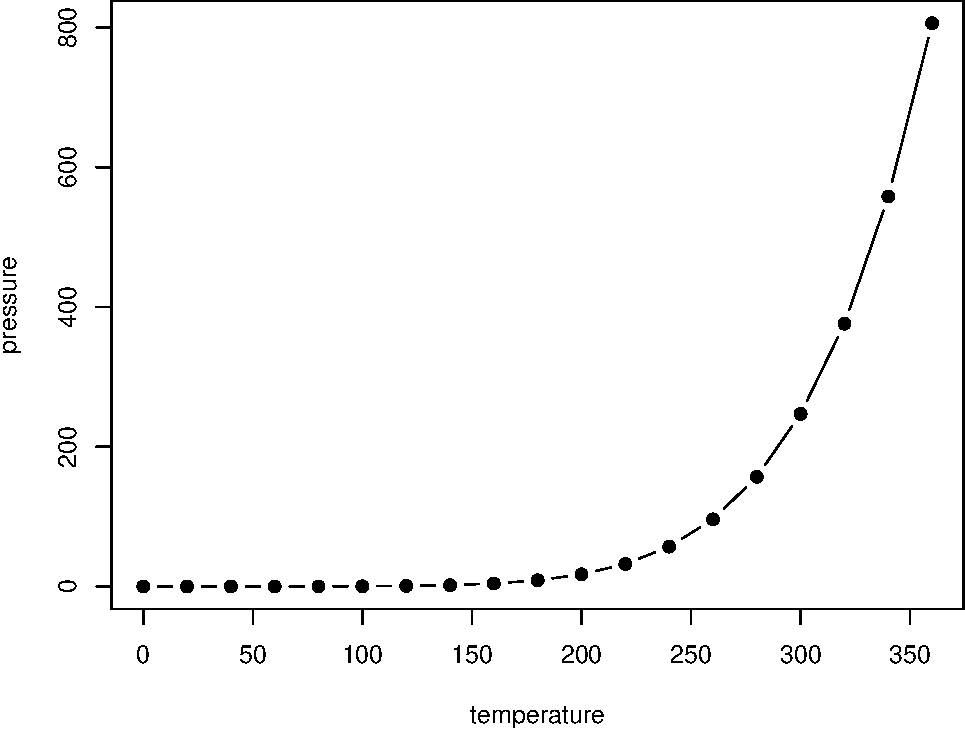
\includegraphics[width=0.8\linewidth]{_main_files/figure-latex/nice-fig-1} 

}

\caption{Here is a nice figure!}\label{fig:nice-fig}
\end{figure}

Don't miss Table \ref{tab:nice-tab}.

\begin{Shaded}
\begin{Highlighting}[]
\NormalTok{knitr}\SpecialCharTok{::}\FunctionTok{kable}\NormalTok{(}
  \FunctionTok{head}\NormalTok{(pressure, }\DecValTok{10}\NormalTok{), }\AttributeTok{caption =} \StringTok{\textquotesingle{}Here is a nice table!\textquotesingle{}}\NormalTok{,}
  \AttributeTok{booktabs =} \ConstantTok{TRUE}
\NormalTok{)}
\end{Highlighting}
\end{Shaded}

\begin{table}

\caption{\label{tab:nice-tab}Here is a nice table!}
\centering
\begin{tabular}[t]{rr}
\toprule
temperature & pressure\\
\midrule
0 & 0.0002\\
20 & 0.0012\\
40 & 0.0060\\
60 & 0.0300\\
80 & 0.0900\\
\addlinespace
100 & 0.2700\\
120 & 0.7500\\
140 & 1.8500\\
160 & 4.2000\\
180 & 8.8000\\
\bottomrule
\end{tabular}
\end{table}

\hypertarget{settings-and-preparation}{%
\chapter{Settings and preparation}\label{settings-and-preparation}}

\hypertarget{camera-and-tripod-settings-and-preparation}{%
\section{Camera and tripod settings and preparation}\label{camera-and-tripod-settings-and-preparation}}

To obtain the best picture quality for model reconstruction, we need an
optimal combination of the light sensibility of the sensor (ISO), the
duration of exposure and the focal of the objective (F). As mentioned,
it is preferable to use a fixed lens (one that doesn't allow zooming) to
facilitate the model reconstruction in the processing step because the
software can't take zooming into account in the reconstruction process.
Maximizing the light source allows us to use the lowest ISO to get
crisper images. Adapted time exposure to allow the right amount of light
to go to the sensor, avoids low key nor high key photo (under/over
exposed photo). This may be adapted according to the subject (light or
dark colored subject or background) or if different lighting conditions
are used.

To maximize the depth of field without lowering the image quality, using
the manual option on the camera dial, the focal F should be set to F16.
Use the manual focus setting on the side of the lens (Figure
\protect\hyperlink{camera_arrows}{3}) to
avoid camera trigger malfunction when the flowers doesn't land on the
detector. If the flower is off centered during rotation, and the
automatic focus can't focus (on the background) the camera trigger is
prevented with the automatic focus. On manual, the camera will always be
triggered by the turn table, even if the focus isn't optimal. Because
the subject is moving and may be off centered on the turntable, the
focus may need to be adapted while the turn table runs. For this you can
pause the turntable, manually adjust the focus, and resume the spin.

A flexible tripod (Figure \protect\hyperlink{tripod}{4}) is used to adjust several camera heights, high,
middle, and low, close to the subject.

\begin{figure}
\hypertarget{camera_arrows}{%
\centering
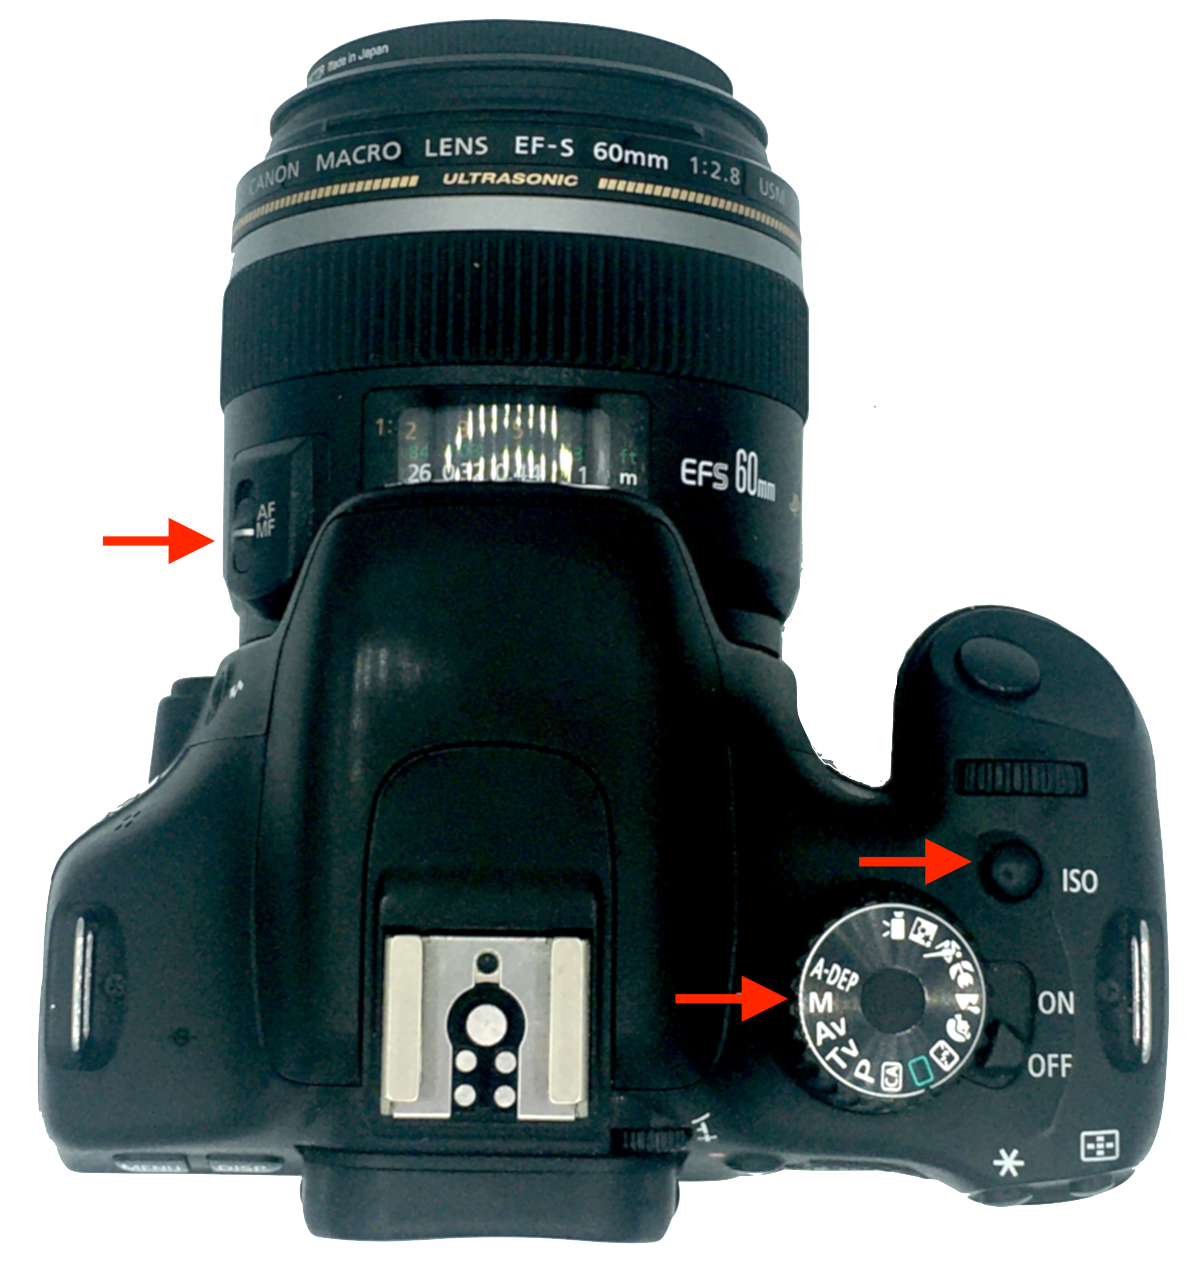
\includegraphics[width=6cm,height=\textheight]{Figures/camera_arrows.png}
\caption{Camera and lens used to take RAW photos. The red arrows (from top to
bottom) depict the button to get manual focus, the ISO button and the
manual parameter on the camera
dial.}\label{camera_arrows}
}
\end{figure}

\begin{figure}
\hypertarget{tripod}{%
\centering
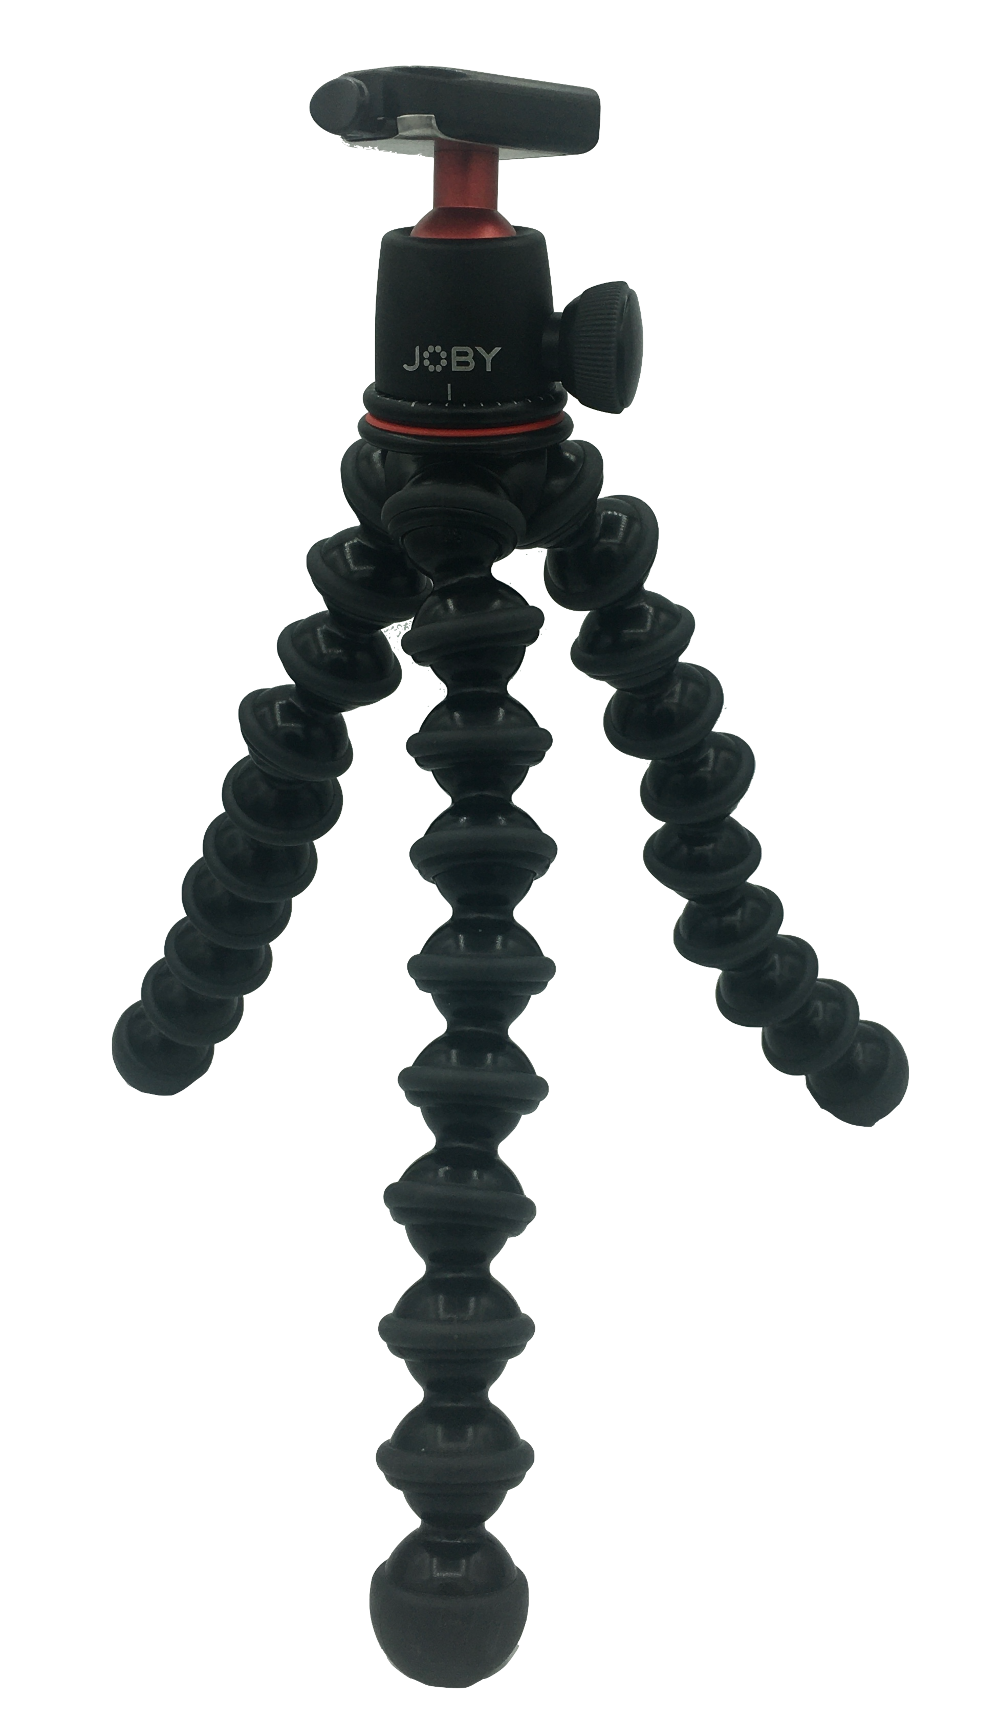
\includegraphics[width=4cm,height=\textheight]{Figures/tripod.png}
\caption{Flexible tripod used to adjust camera
positions.}\label{tripod}
}
\end{figure}

\hypertarget{camera-settings}{%
\subsection{Camera settings}\label{camera-settings}}

The standard settings have to be adjusted depending on the flower
(colour mostly and conditions). We often use the following settings :
exposure time (shutter speed) 1/20s, F/16 focal, ISO 100, standard
exposition on the light meter, and we save pictures as RAW files (ML
setting on the camera display) format to be able to post-process them
for color calibration (Figure \protect\hyperlink{fig:my_label}{5}). A RAW photo of the color chart with an
identical set of lighting conditions and camera settings as the flower
to be photographed is needed for each flower photos series. If several
flowers are processed one after the other without variation of light
conditions, only one chart photo is needed.

The nicer and the sharper the photographs, the easier it will be to
build the models. So make sure that the flower is always in focus. Shade
or high light reflectance can also impair model reconstruction, so pay
attention to these while taking the pictures.

\begin{figure}
\hypertarget{fig:my_label}{%
\centering
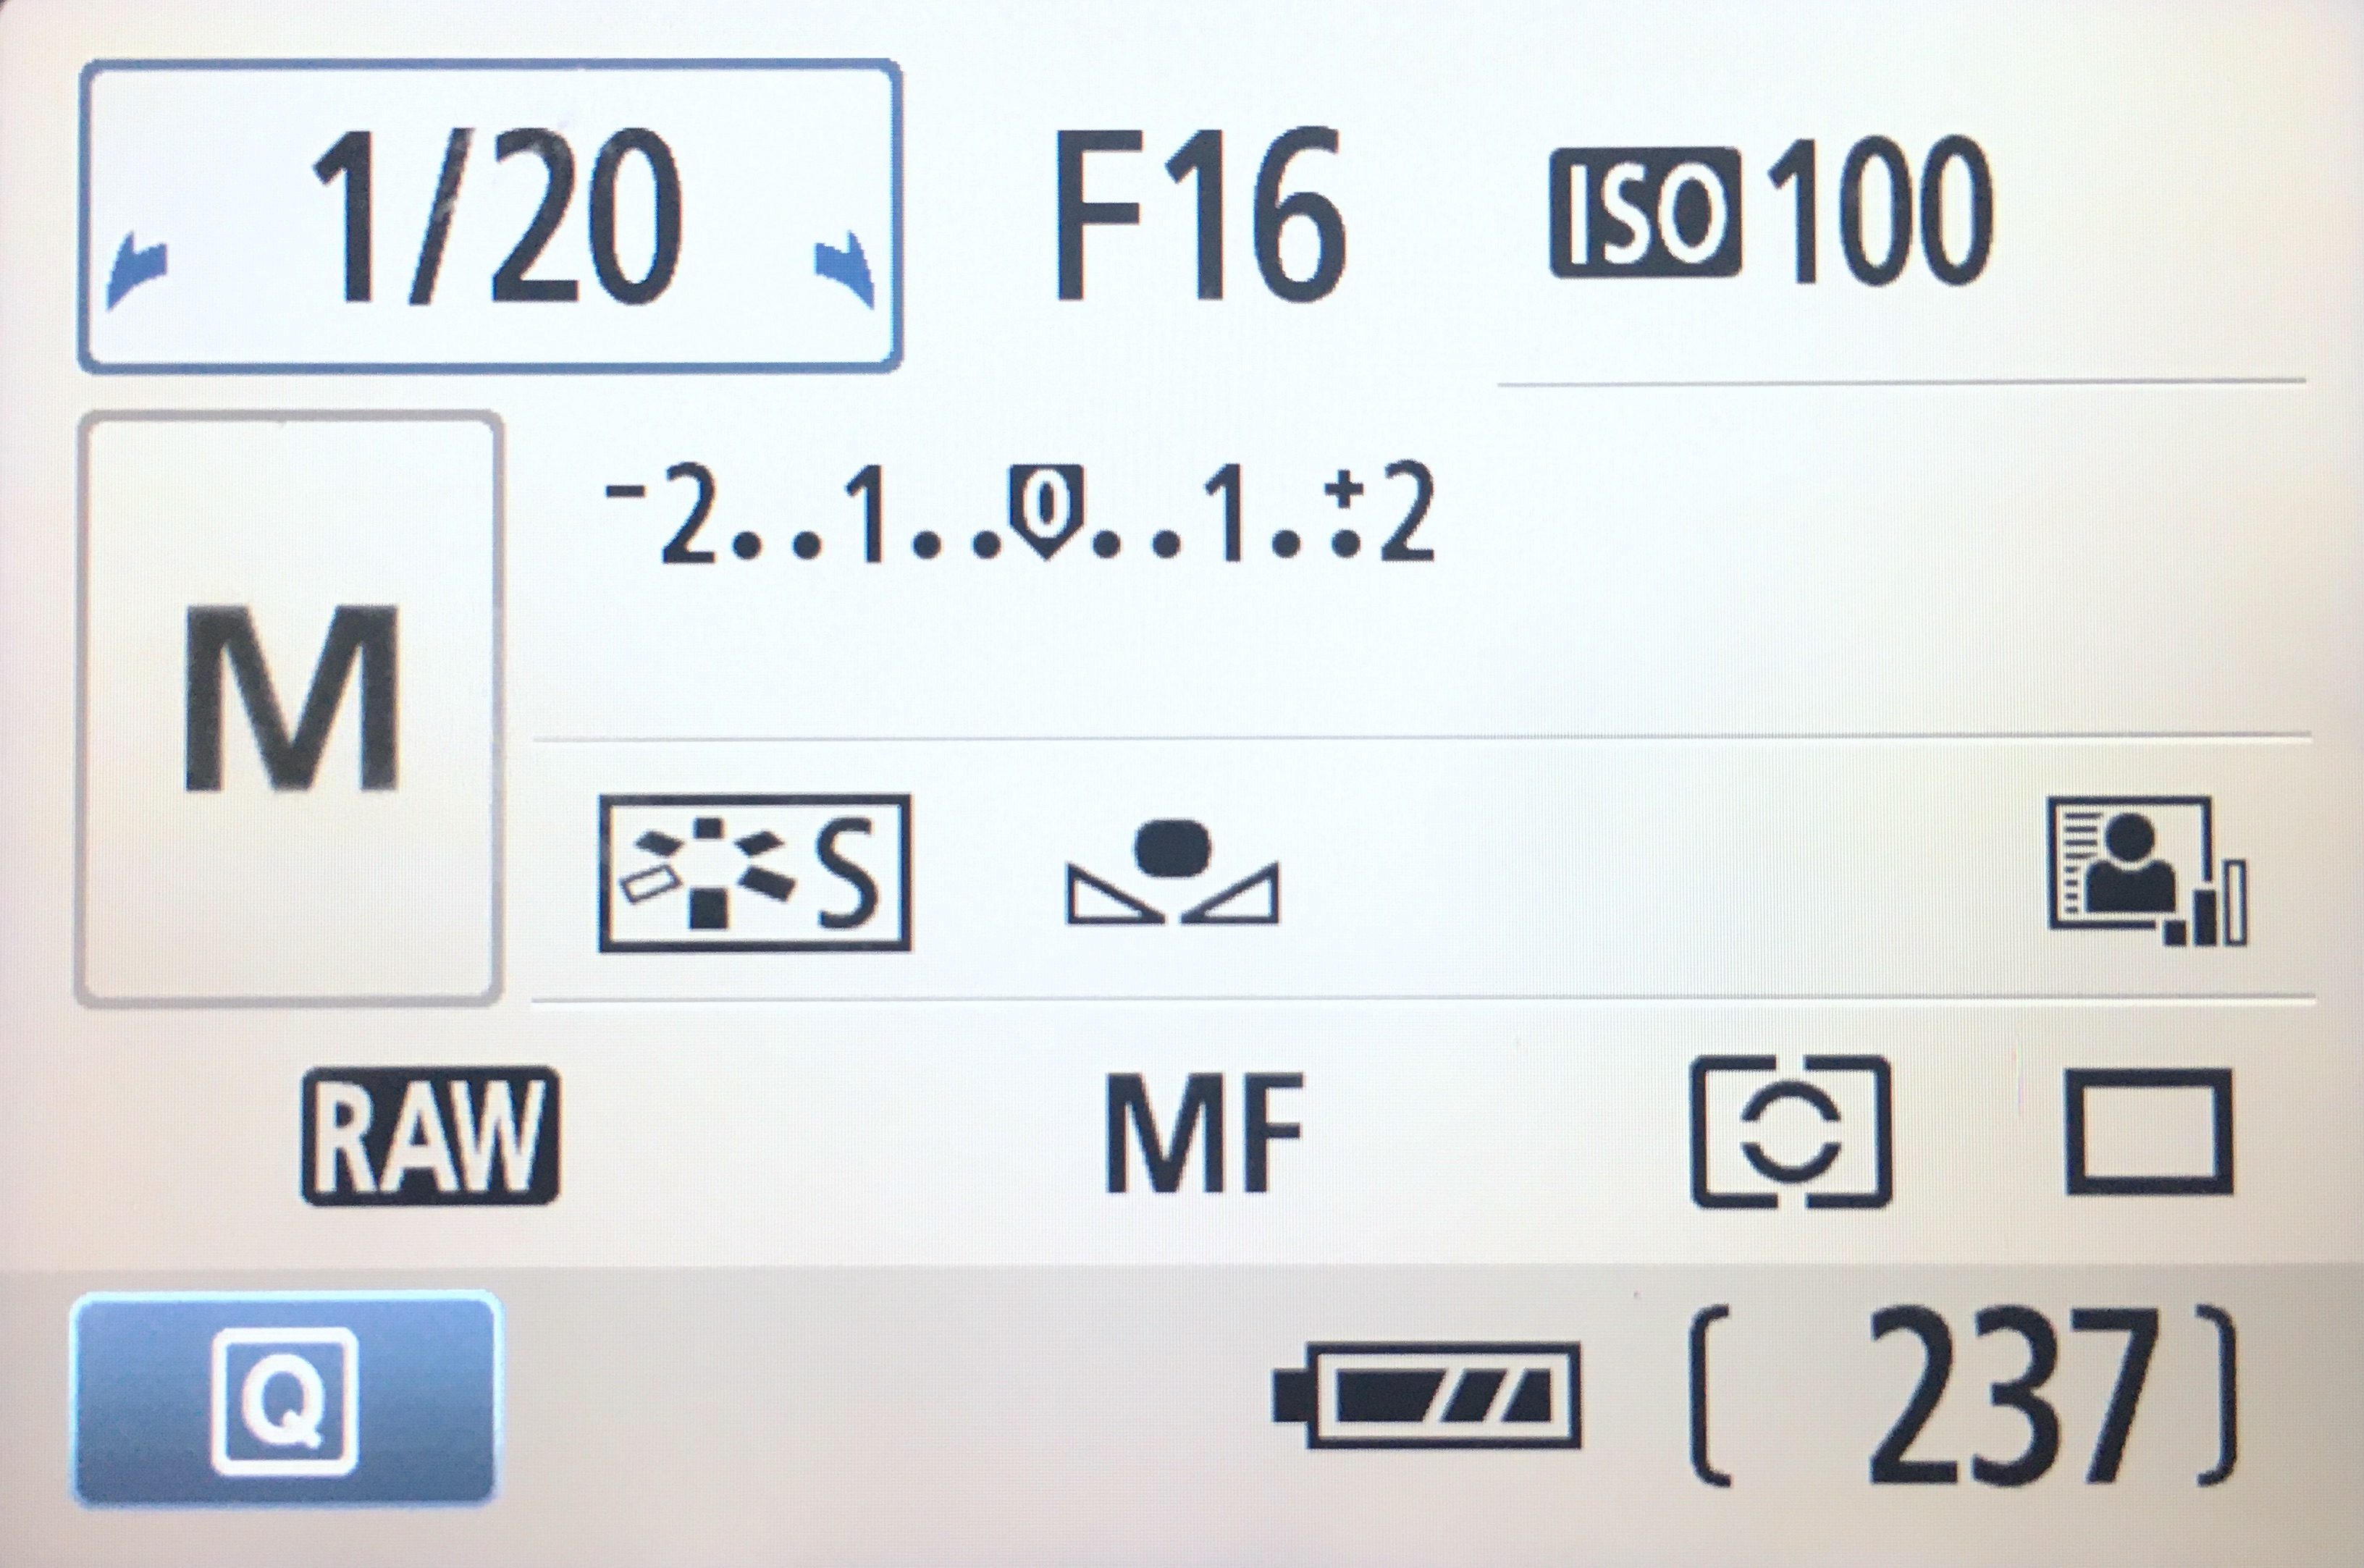
\includegraphics{Figures/camera_settings.JPG}
\caption{Camera settings interface of the Canon
t2i/550D}\label{fig:my_label}
}
\end{figure}

\hypertarget{optional-custom-camera-white-balance}{%
\subsection{Optional : custom camera white balance}\label{optional-custom-camera-white-balance}}

Optionally, you can begin by setting a personalized white balance in
your camera with the light gray scale on the chart :

\begin{enumerate}
\def\labelenumi{\arabic{enumi}.}
\item
  For a Canon camera, take a picture of the gray scale
\item
  Choose \emph{Custom WB} in your camera settings (Figure
  \protect\hyperlink{WB_sub1}{6})
\item
  Select \emph{Custom} and use the picture of the grey scale to define your
  custome white balance (Figure \protect\hyperlink{WB_sub2}{7}). Be careful, you will still require to
  linearize and calibrate each photo afterwards.
\end{enumerate}

However, the color chart will always be the reference for
post-processing the color calibration of each photo. This optional
section only helps to have a better preview of the photos.

\begin{figure}
\hypertarget{WB_sub1}{%
\centering
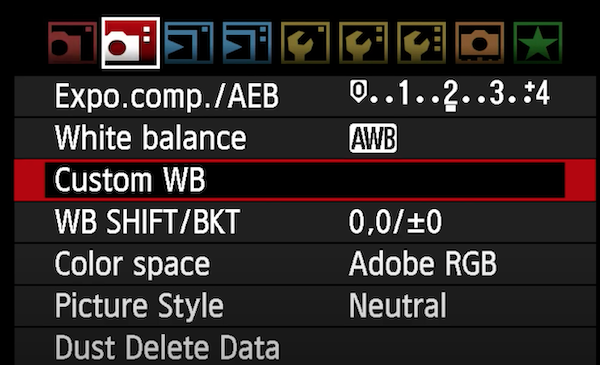
\includegraphics[width=7cm,height=4.5cm]{Figures/Custom WB setting.png}
\caption{Custom WB parameter}\label{WB_sub1}
}
\end{figure}

\begin{figure}
\hypertarget{WB_sub2}{%
\centering
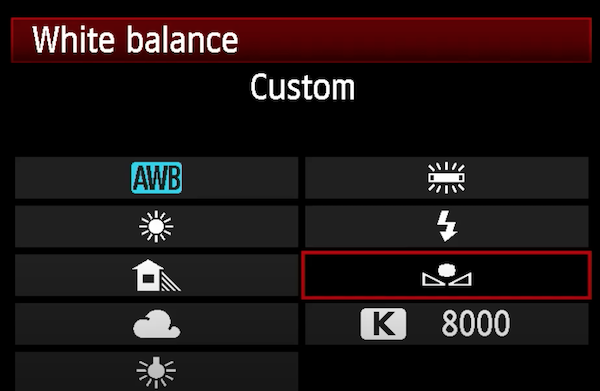
\includegraphics[width=7cm,height=4.5cm]{Figures/Custom WB selection.png}
\caption{Select your custom WB}\label{WB_sub2}
}
\end{figure}

\hypertarget{turn-table-settings-and-preparation}{%
\section{Turn table settings and preparation}\label{turn-table-settings-and-preparation}}

For each run (one 360 spin of the turn table), we use a wait time of 2s
to allow the camera time to save the images on the SD card after it is
triggered, and the flower to stabilize after each rotation.

\begin{enumerate}
\def\labelenumi{\arabic{enumi}.}
\item
  Connect the shutter release to your camera and the turntable Syrp
  Genie II (Figure \protect\hyperlink{fig:shutter}{8}).
\item
  Turn the turntable on (to turn it off, hold the \emph{on} button for 3
  seconds).
\item
  Connect the Syrp Genie II to your device, and do the updates if
  required (needs an internet connection).
\item
  Click on \emph{create content} \textgreater{} \emph{turntable} (Figure
  \protect\hyperlink{genie_root}{9},
  \protect\hyperlink{genie_content}{10}).
\item
  In parameters (Figure \protect\hyperlink{record}{12}), select 20 photos for each run, and 2s of
  waiting (move-wait-shoot-wait-move). If it is too quick, some
  pictures won't be able to be saved as the camera needs a delay to
  save them on the memory card. The spinning device will take the
  first picture then proceed to a move-shoot-move run until the last
  photo.
\item
  Place the white background circle on the turntable to contrast with
  the flower. If your flower is pale, then use a different background
  (colored or darker). Ideally, the color of the circle should be the
  exact same color of the background of the lightbox as this will help
  when applying masks later.
\end{enumerate}

\begin{figure}
\hypertarget{fig:shutter}{%
\centering
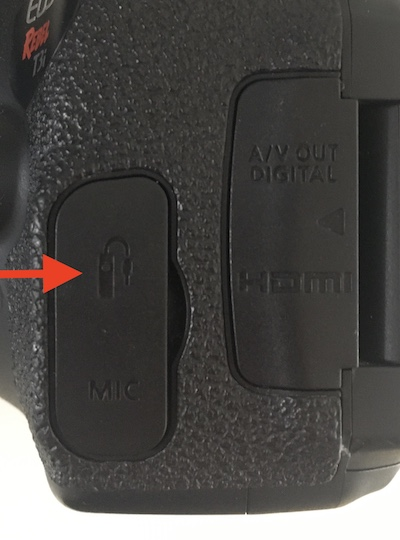
\includegraphics[width=0.3\textwidth,height=\textheight]{Figures/shutter.jpg}
\caption{Camera shutter release port}\label{fig:shutter}
}
\end{figure}

\begin{figure}
\hypertarget{genie_root}{%
\centering

\includegraphics{Figures/genie_root.PNG}
\caption{Genie app interface root}\label{genie_root}
}
\end{figure}

\begin{figure}
\hypertarget{genie_content}{%
\centering
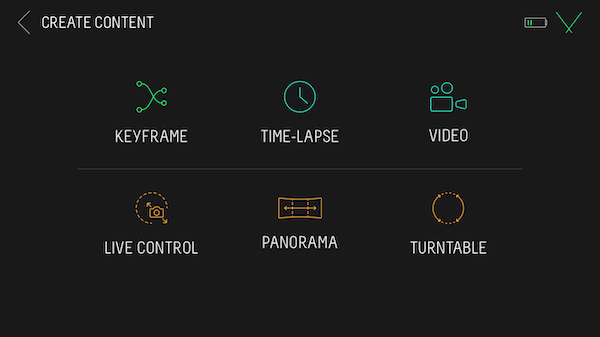
\includegraphics{Figures/genie_create.PNG}
\caption{Create turntable content}\label{genie_content}
}
\end{figure}

\hfill\break

\begin{figure}
\hypertarget{fig:genie_settings}{%
\centering
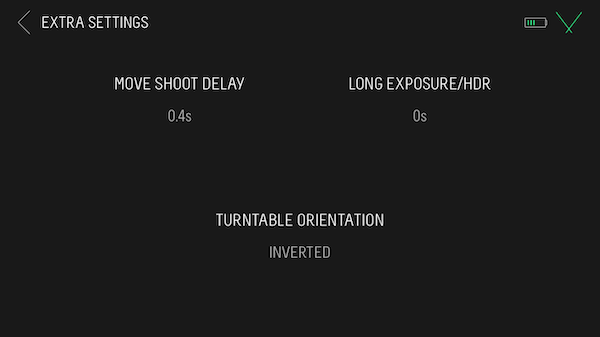
\includegraphics{Figures/genie_settings.PNG}
\caption{Genie detailed
settings}\label{fig:genie_settings}
}
\end{figure}

\begin{figure}
\hypertarget{record}{%
\centering
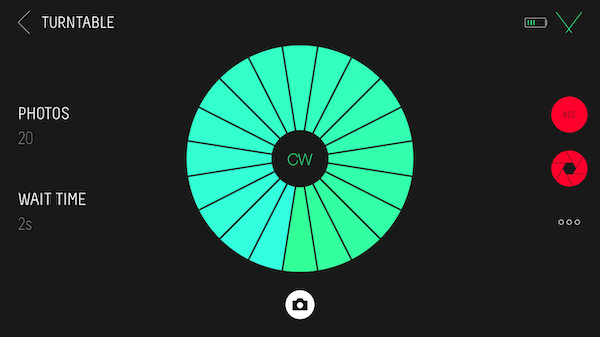
\includegraphics{Figures/genie_turntable_20_1.PNG}
\caption{Start recording with the
turntable}\label{record}
}
\end{figure}

\hypertarget{summary-of-settings}{%
\section{Summary of settings}\label{summary-of-settings}}

L4cm\textbar L12cm \textbf{Parameter} \& \textbf{Description}\\

\begin{center}\rule{0.5\linewidth}{0.5pt}\end{center}

\hfill\break
Aperture \& F/16\\

\begin{center}\rule{0.5\linewidth}{0.5pt}\end{center}

Sensibility \& ISO 100 (lowest)\\

\begin{center}\rule{0.5\linewidth}{0.5pt}\end{center}

Exposure time \& 1/20s - Can be adapted according to the flower.
\textbf{Reminder} : a photo of the color chart in the exact same light
conditions and camera parameters as the flower needs to be taken.\\
\strut \\
Number of photos \& 20 per 360 for one camera position and one flower
position. May be adjusted according to each flower.\\

\begin{center}\rule{0.5\linewidth}{0.5pt}\end{center}

Wait time \& 2s\\

\begin{center}\rule{0.5\linewidth}{0.5pt}\end{center}

\hypertarget{image-capture-step-by-step}{%
\chapter{Image capture step-by-step}\label{image-capture-step-by-step}}

\hypertarget{take-a-picture-of-the-color-chart}{%
\section{Take a picture of the color chart}\label{take-a-picture-of-the-color-chart}}

\begin{enumerate}
\def\labelenumi{\arabic{enumi}.}
\item
  Set the camera settings to F/16, ISO 100, 1/20s, and RAW format.
\item
  Verify that you have enough space on your SD card for RAW photos (a
  minimum of 163 photos, accounting for photos of labels and chart).
\item
  Verify that the placement of your turntable inside the lightbox will
  allow to capture correctly the flower you are about to photograph
  (distance from opening of the lightbox) and that the 1/20s shutter
  speed captures enough light from your flower by taking an initial
  photo of your flower.
\item
  If satisfactory go to next step. The goal here is to have a definite
  set of settings that will match both your flower photos and a color
  chart to subsequently calibrate all your photos that have the same
  light conditions and camera settings.
\item
  Place the color chart where the flower will be placed, without
  shadows, and exposed under the same light as the flower will be
  (angled towards the LED source light in the lightbox). The camera
  settings and lighting cannot be changed after this. If the lighting
  or the camera settings are modified, the color chart needs to be
  taken again to correct the corresponding photos.
\item
  Place the camera so that the entire chart is visible.
\item
  Take a picture of the color chart (RAW). Make sure to Incorporate
  each color squares, and the corners of the chart as follows (Figure
  \protect\hyperlink{colorchart}{13}).
\end{enumerate}

\begin{figure}
\hypertarget{colorchart}{%
\centering
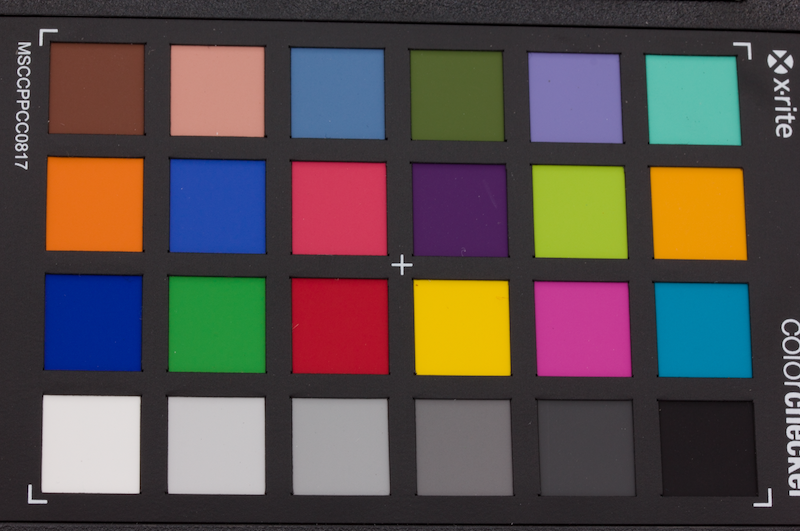
\includegraphics[width=0.3\textwidth,height=\textheight]{Figures/chart_example.png}
\caption{Colour chart photo taken at the beginning of the process to calibrate
the photos in post process.}\label{colorchart}
}
\end{figure}

\hypertarget{flower-placement-image-capture}{%
\section{Flower placement \& Image capture}\label{flower-placement-image-capture}}

To reconstruct an accurate 3D model, it is very important to have
pictures of all the parts and details of the flowers and from several
angles. Also, the photographs need to overlap with each other for proper
alignment in the first steps of the reconstruction. For this reason,
several pictures will be taken of each flower: from different
orientation and all around the flower. We suggest that flowers should be
photographed from at least two positions. Note that it is better to take
more photos than less because if we can drop some pictures during the
model reconstruction, it is impossible to come back and take more
pictures if we realize that we should have taken more.

For Gesneriaceae, we first suggest a standard orientation and an
upside-down position of the flower as this generally gives satisfactory
results (Figure
\protect\hyperlink{flowerplacement_2}{\[flowerplacement_2\]}). For more complex flowers, three
positions may be required: horizontal, vertical, and upside down (Figure
\protect\hyperlink{flowerplacement_3}{\[flowerplacement_3\]}).

\begin{enumerate}
\def\labelenumi{\arabic{enumi}.}
\item
  Clip the camera on the flexible tripod (gorillapod) and place the
  camera at one of the three position required per flower position :
  high mid, and low position (see Figure
  \protect\hyperlink{flowerplacement_2}{\[flowerplacement_2\]}). Make sure to not use different
  camera orientations (landscape vs.~portrait).
\item
  If sepals need to be removed, use a razor blade to cut them at the
  base and mark the sepal intersections with a waterproof pen to keep
  track of the morphological structures.
\item
  Pin the flower through the peduncle or the floral receptacle and
  through a block of dense foam or malleable gum. You can use several
  pins to avoid any sliding of the flower during the image capture
  process.
\item
  Make sure to place the flower so that the whole flower will be
  encompassed in the camera frame as much as possible. It is best to
  have the subject to take the most place as possible in the camera
  frame to capture every details overall than having it entirely in
  the camera frame but with poor detail quality. What counts the most
  is to get several overlapping photos for each features. Make sure
  that the flower is not in contact with anything as this would deform
  the flower and create problems during the model reconstruction.
\item
  For flowers with very uniform color or with radial symmetry, it may
  be important to place dots with a waterproof pen on the corolla to
  facilitate manual marker positioning and/or automated pixel position
  detection in the reconstruction step.
\item
  Place a scale (e.g., 1 cm) directly below the flower.
\item
  Take a picture of the flower with the label for each new positioning
  of the flower. This will help to identify each group of images in
  the following model construction.
\item
  Press the \emph{rec} button on your smartphone using the turntable
  interface to start the spin of the turntable and automated image
  capture.
\item
  Verify occasionally the focus on the flower while the flower rotates
  by pressing the square button (stop) and manually adjust the focus
  if needed, then press rec to resume your spin.
\end{enumerate}

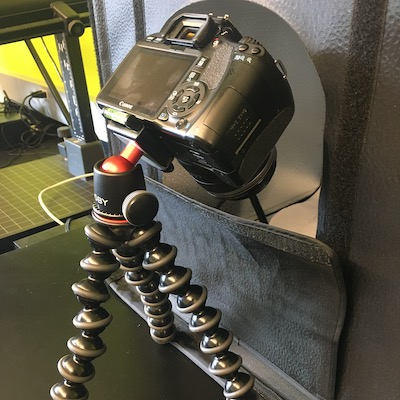
\includegraphics[width=0.9\textwidth,height=\textheight]{Figures/camera_position_1.JPG}

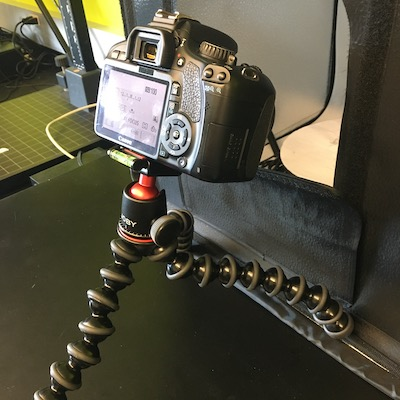
\includegraphics[width=0.9\textwidth,height=\textheight]{Figures/camera_position_2.JPG}

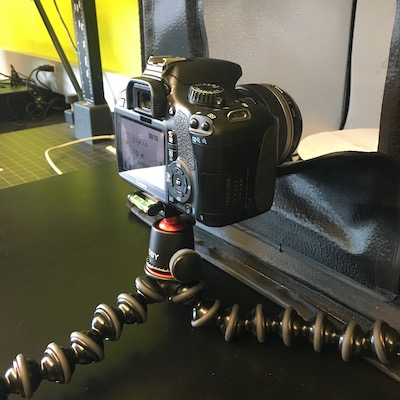
\includegraphics[width=0.9\textwidth,height=\textheight]{Figures/camera_position_3.JPG}

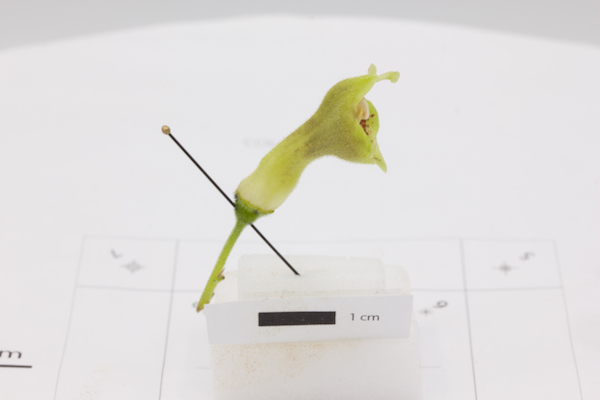
\includegraphics[width=0.9\textwidth,height=\textheight]{Figures/position_2.jpg}

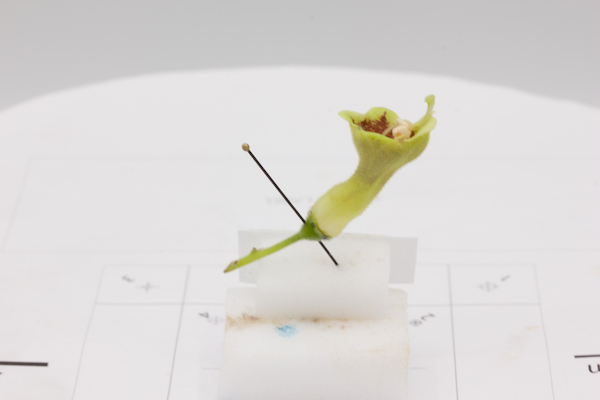
\includegraphics[width=0.9\textwidth,height=\textheight]{Figures/position_5.jpg}

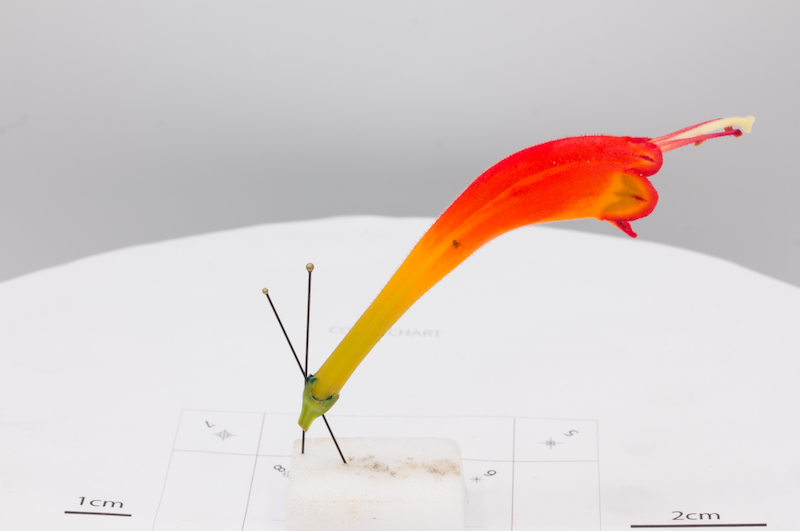
\includegraphics[width=0.9\textwidth,height=\textheight]{Figures/flowerplacement_1.png}

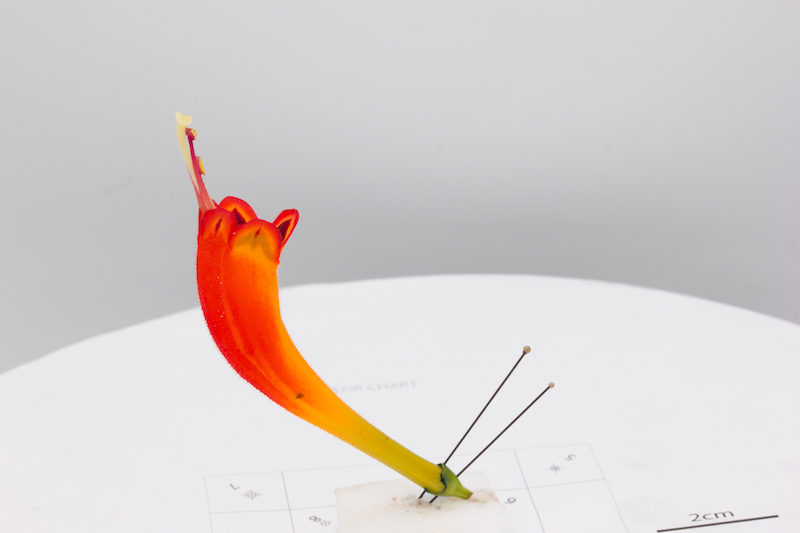
\includegraphics[width=0.9\textwidth,height=\textheight]{Figures/flowerplacement_2.jpg}

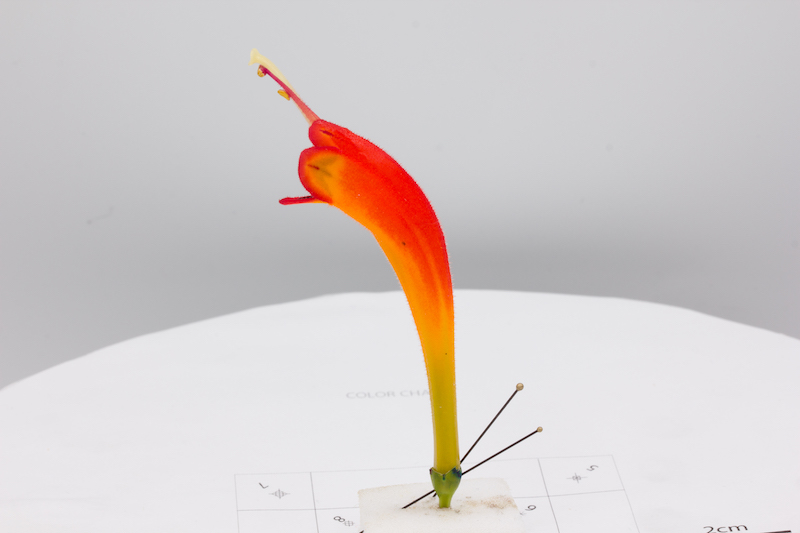
\includegraphics[width=0.9\textwidth,height=\textheight]{Figures/flowerplacement_3.jpg}

Adjust the number of flower positions and number of photos according to
each flower. For intricate flowers, or flowers that can't be captured
entirely with only two positions (ventral and dorsal), you can place the
flower on an another position (Figure
\protect\hyperlink{3placement}{14}). On the
contrary, if the flower can't be placed on several positions, you may
need to increase the number of photos per camera height in order to have
sufficient information for the software to reconstruct accurate 3D
models.

\hypertarget{footnotes-and-citations}{%
\chapter{Footnotes and citations}\label{footnotes-and-citations}}

\hypertarget{footnotes}{%
\section{Footnotes}\label{footnotes}}

Footnotes are put inside the square brackets after a caret \texttt{\^{}{[}{]}}. Like this one \footnote{This is a footnote.}.

\hypertarget{citations}{%
\section{Citations}\label{citations}}

Reference items in your bibliography file(s) using \texttt{@key}.

For example, we are using the \textbf{bookdown} package \citep{R-bookdown} (check out the last code chunk in index.Rmd to see how this citation key was added) in this sample book, which was built on top of R Markdown and \textbf{knitr} \citep{xie2015} (this citation was added manually in an external file book.bib).
Note that the \texttt{.bib} files need to be listed in the index.Rmd with the YAML \texttt{bibliography} key.

The RStudio Visual Markdown Editor can also make it easier to insert citations: \url{https://rstudio.github.io/visual-markdown-editing/\#/citations}

\hypertarget{image-post-processing}{%
\chapter{Image post processing}\label{image-post-processing}}

\hypertarget{file-names-and-storage}{%
\section{File names and storage}\label{file-names-and-storage}}

We found that it is critical to have a very organized structure for
saving files, especially when several persons are working on the same
project. We propose here what has been working so far for us.

In a species folder named with the name of the species
(\emph{Genus\_species}), there should be a distinct folder for each individual
photographed, usually with a different collection number. If the same
individual has been photographed several times, the date of photos
acquisition should be appended to the folder name to discriminate them.
We also indicate with the folder name if the individual has been
photographed with or without sepals.

For each flower, we have one folder for uncalibrated photos, one for
calibrated photos, and one for the model. The picture of the color chart
should be placed in the uncalibrated photos.

To distinguish which photo goes in which chunk, a photo of the label is
taken at the beginning of each chunk (each set of photo per side of
flower). We suggest to place the photos from different chunks in
different folders, once the photos are calibrated. The date of when the
photos are taken is important because it helps matching the calibration
to the right DNG file. If more than one set of photos with different
lighting or camera settings are taken, make sure to distinguish the
color charts that correspond to each set of photos.

Genus\_species\\
GEN\_species\_CollectionNumber\\
sepal\_DD.MM.YYYY or no\_sepals\_DD.MM.YYYY\\
Model\\
\emph{MetashapeProject}\\
\emph{MetashapeProjectFolder.files}\\
\emph{model.obj}\\
\emph{model.ply}\\
\emph{texture.jpg}\\
Photos calibrated\\
\emph{Place here all the calibrated photos, that you can organize per chunk}\\
Photos to calibrate\\
\emph{Place here all the RAW photos and color chart}\\

\hypertarget{image-color-calibration}{%
\section{Image color calibration}\label{image-color-calibration}}

\hypertarget{creating-color-profiles}{%
\subsection{Creating color profiles}\label{creating-color-profiles}}

We present here three ways to create camera profiles. The first one
allows to manually check the automatic detection of the color chart, the
second and third ones are fully automatic (on MacOS and windows
respectively).

This does not linearize the photos. For further details on color
calibration read \citep{troscianko2015image}.

\textbf{Method 1 : Manual creation of color profiles}

\begin{enumerate}
\def\labelenumi{\arabic{enumi}.}
\item
  Get the \href{https://xritephoto.com/ph_product_overview.aspx?ID=938\&Action=Support\&SoftwareID=2030}{Xrite ColorChecker Camera Calibration
  software}
  and \href{https://helpx.adobe.com/photoshop/using/adobe-dng-converter.html}{Adobe DNG converter
  software}.
\item
  Create a new empty folder called DNG.
\item
  Copy the RAW file representing your color chart in your DNG folder,
  and rename it accordingly (e.g.~Color\_chart\_DD.MM.YYYY).
\item
  Open DNG converter and select the DNG folder we created for the
  first box. You need to select a folder, and can't select a specific
  file, the software will convert all the files within this folder.
  Default parameters are ok for step 2-4. It will export the RAW file
  in the DNG folder to a DNG file with the same file name (Figure
  \protect\hyperlink{adobe_dng}{15}).
\item
  Open the Color Checker Camera Calibration software and drag and drop
  the newly created DNG file in the software. The software will
  automatically draw a grid around it. Make sure that the green grid
  fits the chart, avoiding edge effects on each square of color
  (Figure \protect\hyperlink{color_checker_camera_calibration}{16}).
\item
  Click on \emph{create profile} and save it under Color\_Chart\_DD.MM.YYYY
  (Figure \protect\hyperlink{color_checker_profile}{17}).
\end{enumerate}

\begin{figure}
\hypertarget{adobe_dng}{%
\centering
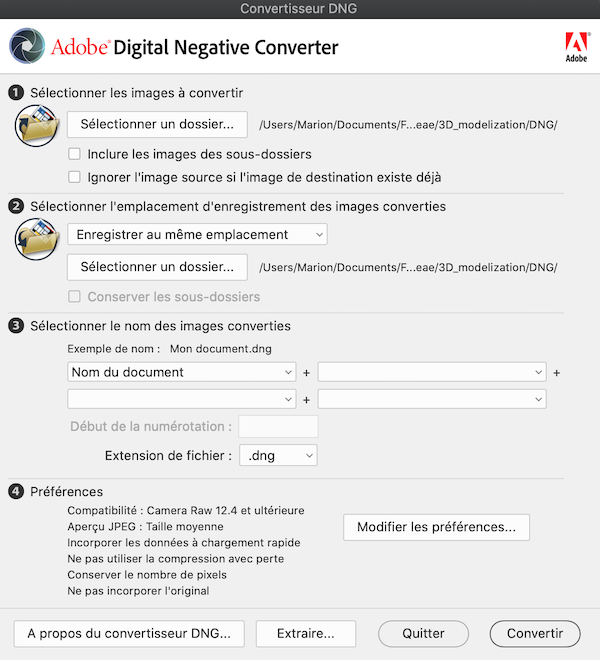
\includegraphics[width=1\textwidth,height=\textheight]{Figures/AdobeDNGConverter.png}
\caption{Convert RAW chart to DNG in Adobe DNG
Converter}\label{adobe_dng}
}
\end{figure}

\begin{figure}
\hypertarget{color_checker_camera_calibration}{%
\centering
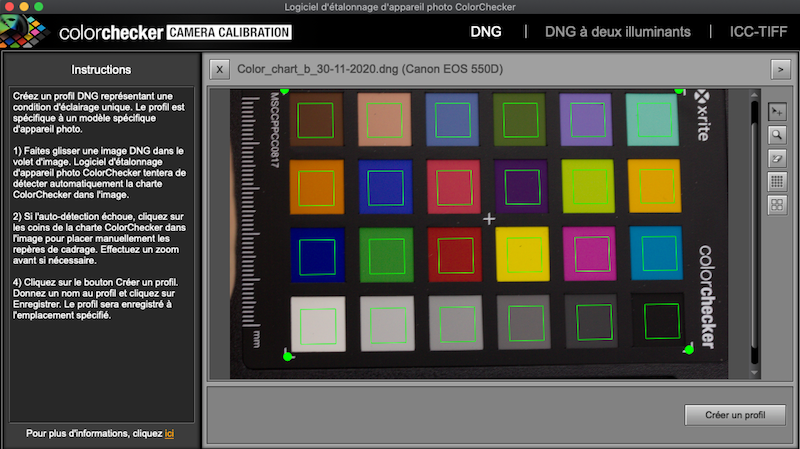
\includegraphics[width=1\textwidth,height=\textheight]{Figures/ColorChecker camera cailbration.png}
\caption{Align grid on chart in ColorChecker Camera
Calibration}\label{color_checker_camera_calibration}
}
\end{figure}

\begin{figure}
\hypertarget{color_checker_profile}{%
\centering
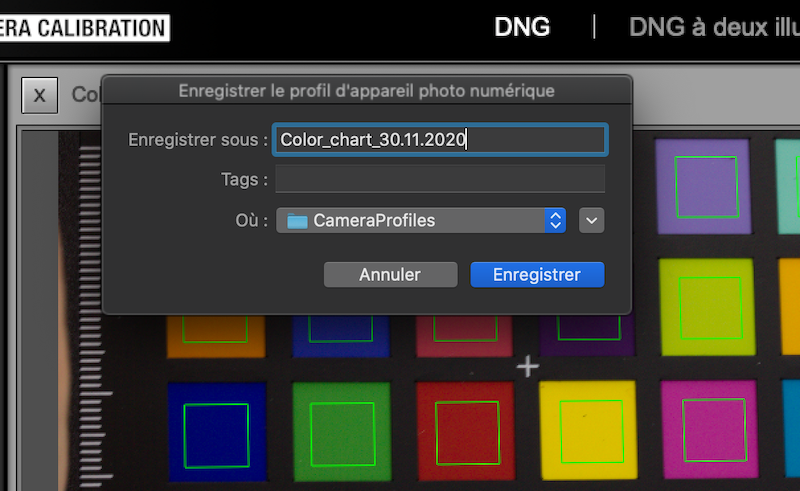
\includegraphics[width=1\textwidth,height=\textheight]{Figures/create profile.png}
\caption{Export the color
profile}\label{color_checker_profile}
}
\end{figure}

\begin{figure}
\hypertarget{fig:workflow}{%
\centering
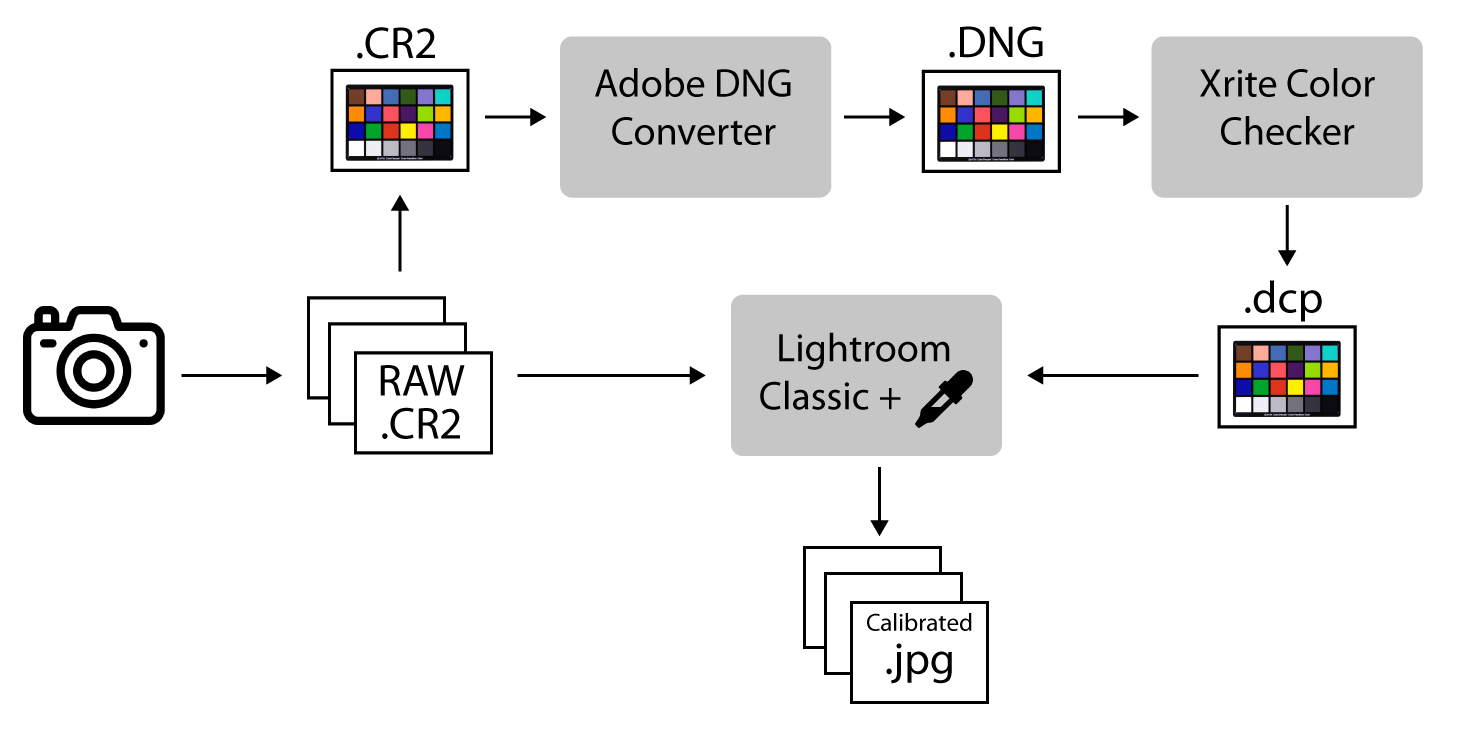
\includegraphics[width=0.8\textwidth,height=\textheight]{Figures/manual_method.png}
\caption{Image color calibration
workflow}\label{fig:workflow}
}
\end{figure}

\textbf{Method 2 : X-Rite Color Checker plug-in installation and automatic
creation of color profiles on MacOS}

\begin{enumerate}
\def\labelenumi{\arabic{enumi}.}
\item
  Directly in Adobe Lightroom, you can add ColorChecker Camera
  Calibration as a module to a means of exporting files directly into
  a color profile.

  \begin{enumerate}
  \def\labelenumii{\arabic{enumii}.}
  \item
    Click on File \textgreater{} Export \textgreater{} \emph{Plug-in Manager} (or \emph{gestionnaire
    des modules externes} in the left bottom corner)
  \item
    Click on \emph{Add}
  \item
    Navigate to \emph{Library} \textgreater{} \emph{Application Support} \textgreater{} \emph{Adobe} \textgreater{}
    \emph{Lightroom} \textgreater{} \emph{Modules}
  \item
    Select \emph{XRiteColorCheckerPassport.lrplugin} and then click on
    \emph{Add Plug-in} and \emph{done}.
  \end{enumerate}
\item
  Click on the color chart then \emph{File} \textgreater{} \emph{Export} \textgreater{} Choose \emph{Xrite
  presets} from the drop down menu.
\item
  Name your profile then \textgreater{} \emph{Export}
\item
  It will go through ColorCheckerCamera calibration to automatically
  create the profile.
\item
  Restart Lightroom as indicated.
\end{enumerate}

\textbf{Method 3 : X-Rite Color Checker plug-in installation and automatic
creation of color profiles on Windows}

\begin{enumerate}
\def\labelenumi{\arabic{enumi}.}
\item
  Get the \href{https://xritephoto.com/ph_product_overview.aspx?ID=938\&Action=Support\&SoftwareID=2030}{Xrite ColorChecker Camera Calibration
  software}
  and download the \emph{PC Version}. Save the \emph{CameraCalibrationSetup.exe}
  in your downloads, for example, and run the program.
\item
  If Adobe Lightroom Classic is already installed on your computer,
  the installation program should proposed you to install the Adobe
  Photoshop Lightroom plug-in (Figure
  \protect\hyperlink{color_checker_plug_in_win}{19}). Install it.
\item
  Once the plug-in is installed, run Adobe Lightroom Classic and
  import your color chart (\emph{File} \textgreater{} \emph{Import}).
\item
  Click on \emph{File} \textgreater{} \emph{Export} and in the drop-down menu, select
  \emph{X-Rite Preselection} (Figure
  \protect\hyperlink{x_rite_preselection}{20}). Name your profile, and click on
  \emph{Export}.
\item
  Restart Lightroom as indicated.
\item
  Run the setps 4 and 5 each time you want to create a new color
  profile witht the color chart.
\end{enumerate}

\begin{figure}
\hypertarget{color_checker_plug_in_win}{%
\centering
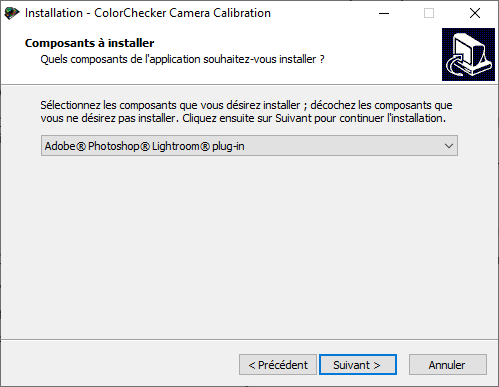
\includegraphics[width=\textwidth,height=7cm]{Figures/color_checker_plug_in_win.png}
\caption{Color Checker plug-in for Lightroom
installation}\label{color_checker_plug_in_win}
}
\end{figure}

\begin{figure}
\hypertarget{x_rite_preselection}{%
\centering
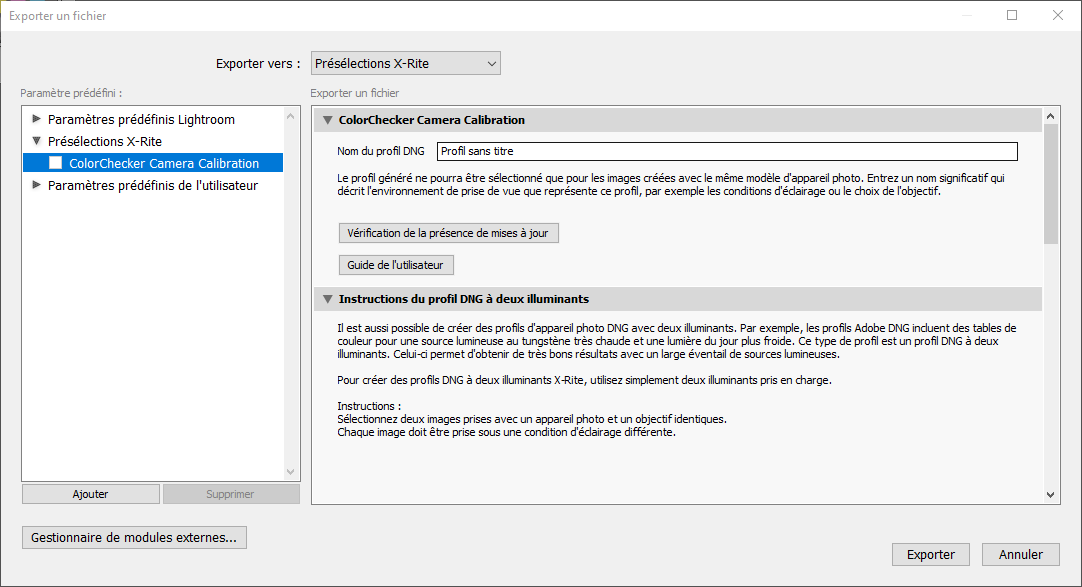
\includegraphics[width=\textwidth,height=7cm]{Figures/x_rite_preselection.png}
\caption{Color chart profile
exportation}\label{x_rite_preselection}
}
\end{figure}

\hypertarget{color-and-illuminance-calibration-from-profiles}{%
\subsection{Color and illuminance calibration from profiles}\label{color-and-illuminance-calibration-from-profiles}}

\begin{enumerate}
\def\labelenumi{\arabic{enumi}.}
\item
  Import your photos in Lightroom Classic. \emph{File} \textgreater{} \emph{Import} then
  select your folder of RAW photos.
\item
  Select the tab \emph{development}.
\item
  Select the photo of the chart
\item
  Select the color profile corresponding to the color chart you have
  selected (see Figure
  \protect\hyperlink{colorux5cux2520profile}{\[color profile\]} to manually add a color profile) to
  calibrate the photo of the chart with its own calibration profile.

  \begin{figure}
  \hypertarget{add_profile}{%
  \centering
  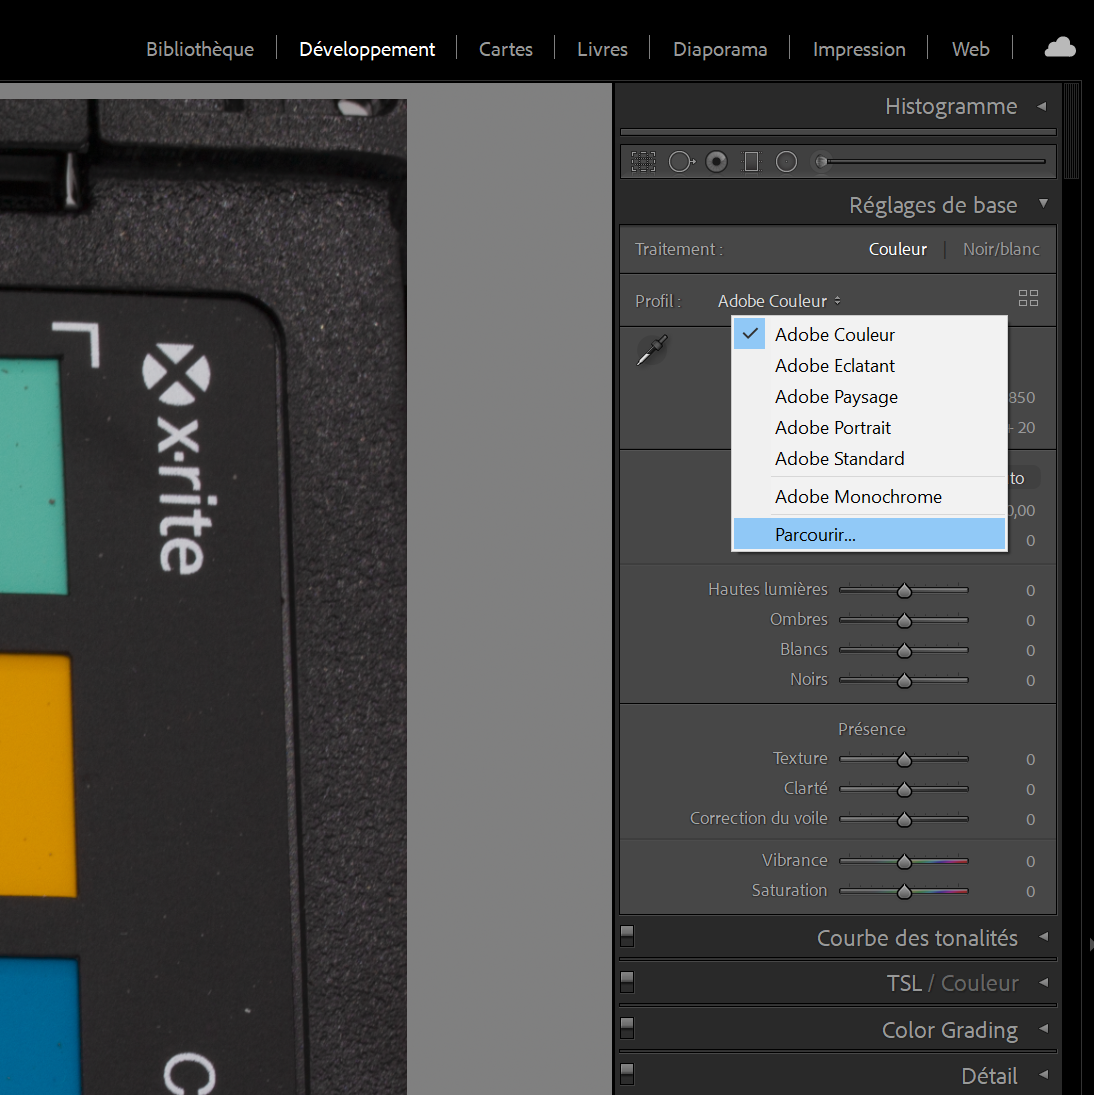
\includegraphics[width=\textwidth,height=7cm]{Figures/profil_capture_1.png}
  \caption{Add a new color
  profile}\label{add_profile}
  }
  \end{figure}

  \begin{figure}
  \hypertarget{settings_synchronize}{%
  \centering
  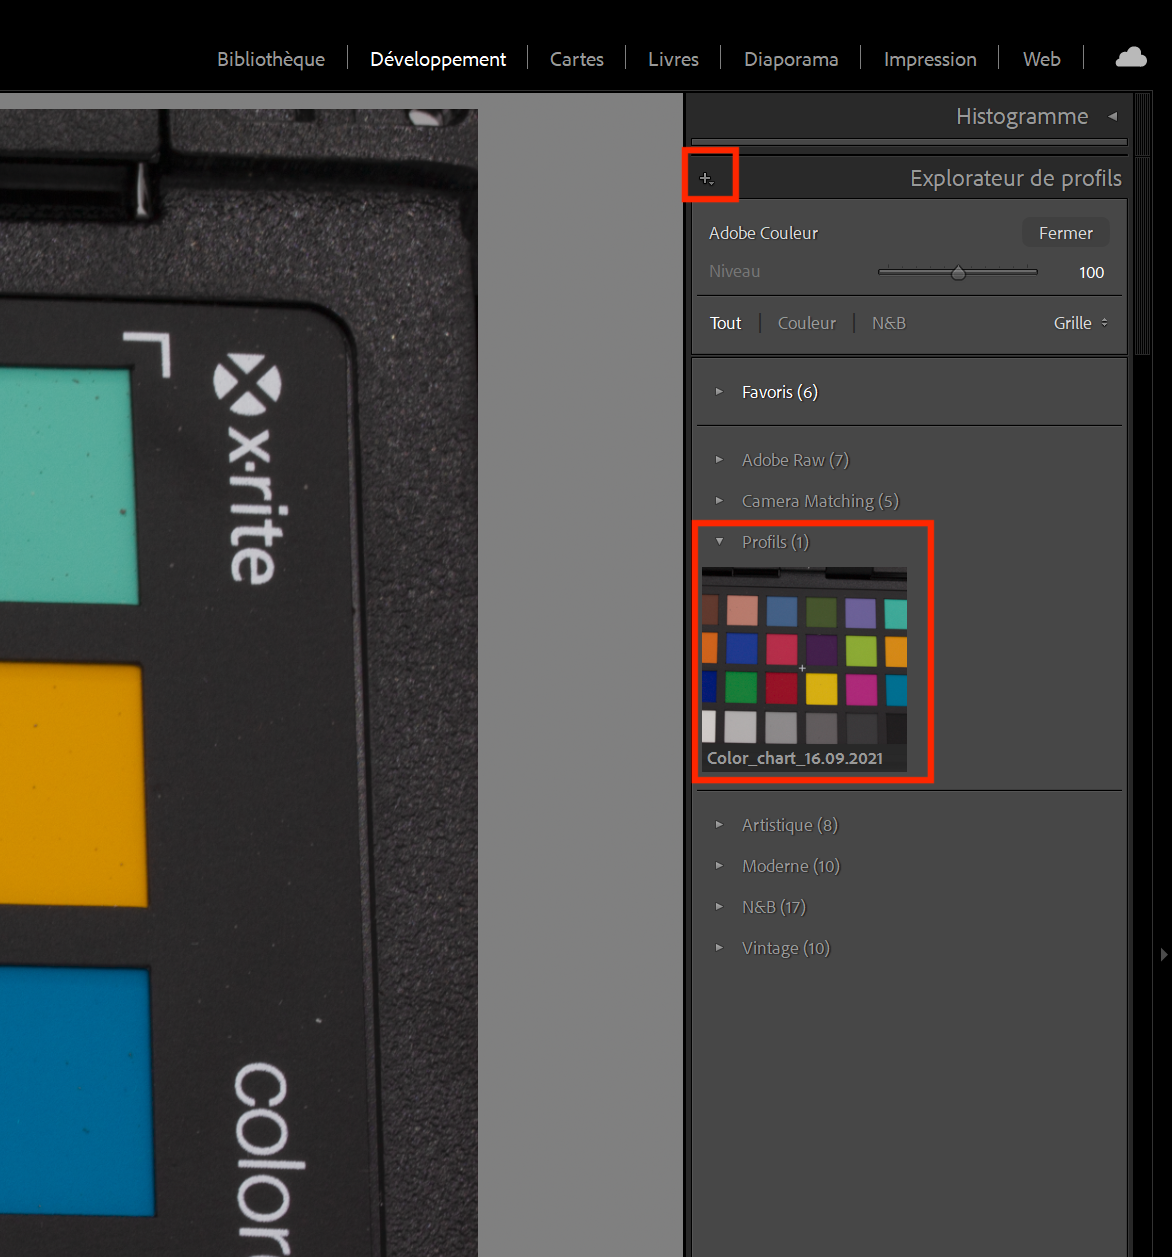
\includegraphics[width=\textwidth,height=7cm]{Figures/profil_capture_2.png}
  \caption{After adding a profile with the + sign, select it in the list
  below.}\label{settings_synchronize}
  }
  \end{figure}
\item
  Use the eyedropper over the 75\% gray scale (the last one before the
  black chip on the color chart, see Figure
  \protect\hyperlink{fig:xrite_description}{2}). Do not click on the photo with
  the eye dropper, only hover over the photo.
\item
  Select the exposition setting, and adjust the values the eyedropper
  indicates of the gray scale using the exposition setting to obtain
  the RGB values of the closest values to 0.33 0.33 0.33
  (corresponding to 85/255 for each of the red, blue, and green
  class). The illuminance is now adjusted in addition to the color
  calibration, but only on the chart.
\item
  To apply the modifications we just did to all the photos, select all
  the photos (Cmd+A or Ctrl+A), and make sure that the one for which
  you made changes is highlighted (in white compared to light gray for
  the other ones selected) (see Figure
  \protect\hyperlink{fig:synchronize}{23}). Check the profiles and exposure boxes
  before synchronizing to all the other photos.
\item
  Click on the button \emph{synchronize}.
\end{enumerate}

\begin{figure}
\hypertarget{fig:synchronize}{%
\centering
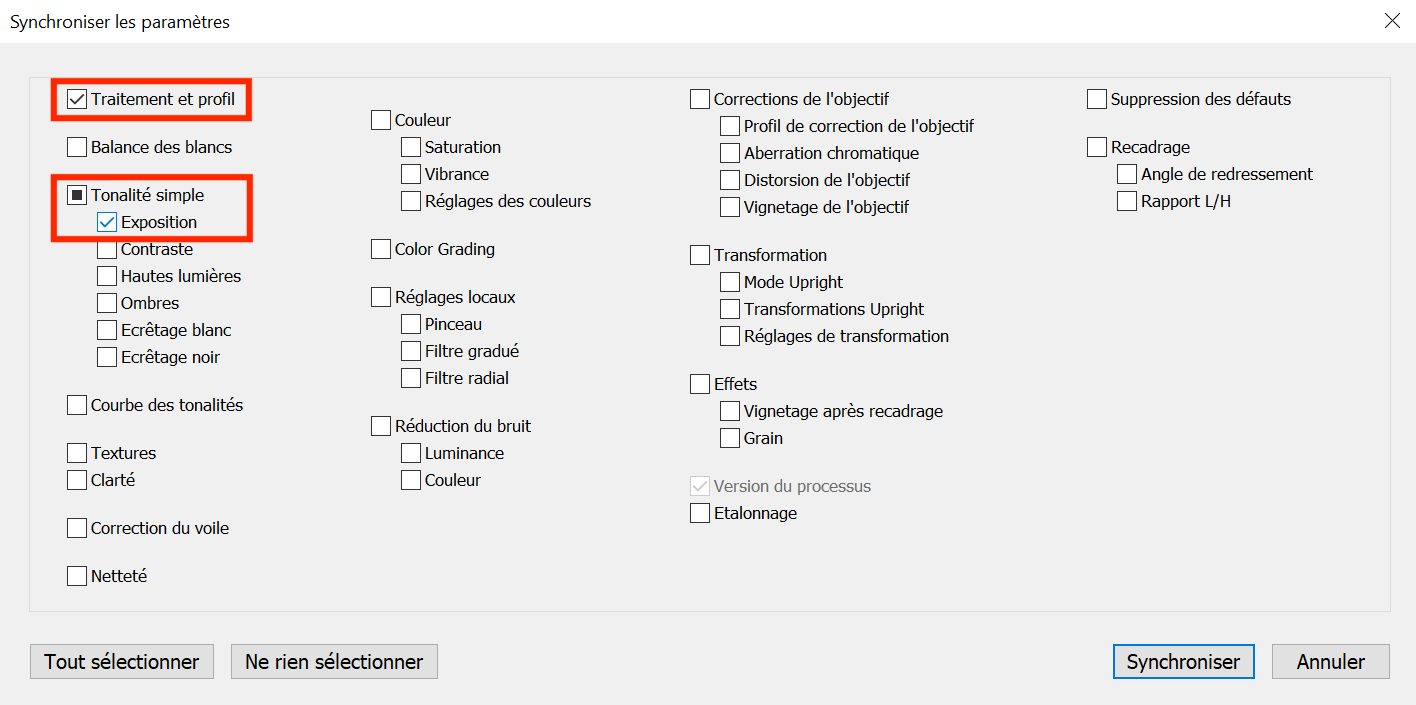
\includegraphics{Figures/synchronize_capture.png}
\caption{Synchronize your settings made to the photo of the chart to all the
other photos and check the two categories you modified (color profile
and exposure).}\label{fig:synchronize}
}
\end{figure}

\hypertarget{export-calibrated-files-to-jpg-format}{%
\subsection{Export calibrated files to jpg format}\label{export-calibrated-files-to-jpg-format}}

\begin{enumerate}
\def\labelenumi{\arabic{enumi}.}
\item
  Select all the photos you need to export or all of them (cmd+A or
  windows+A)
\item
  Click on \emph{File} \textgreater{} \emph{Export}
\item
  You can create presets that you will only need to create once to
  always export the same way in Adobe Lightroom (example Figure
  \protect\hyperlink{export_parameters}{24}), and add personalized file names
  such as \_color\_calibrated at the end of each .jpg file (see also
  for that Figure \protect\hyperlink{export_parameters}{24}).
\item
  In their own folder, you can then sort the calibrated photos for
  color and exposure per chunks (easily distinguishable by the
  separation created by a photo of the label).
\end{enumerate}

\begin{figure}
\hypertarget{export_parameters}{%
\centering
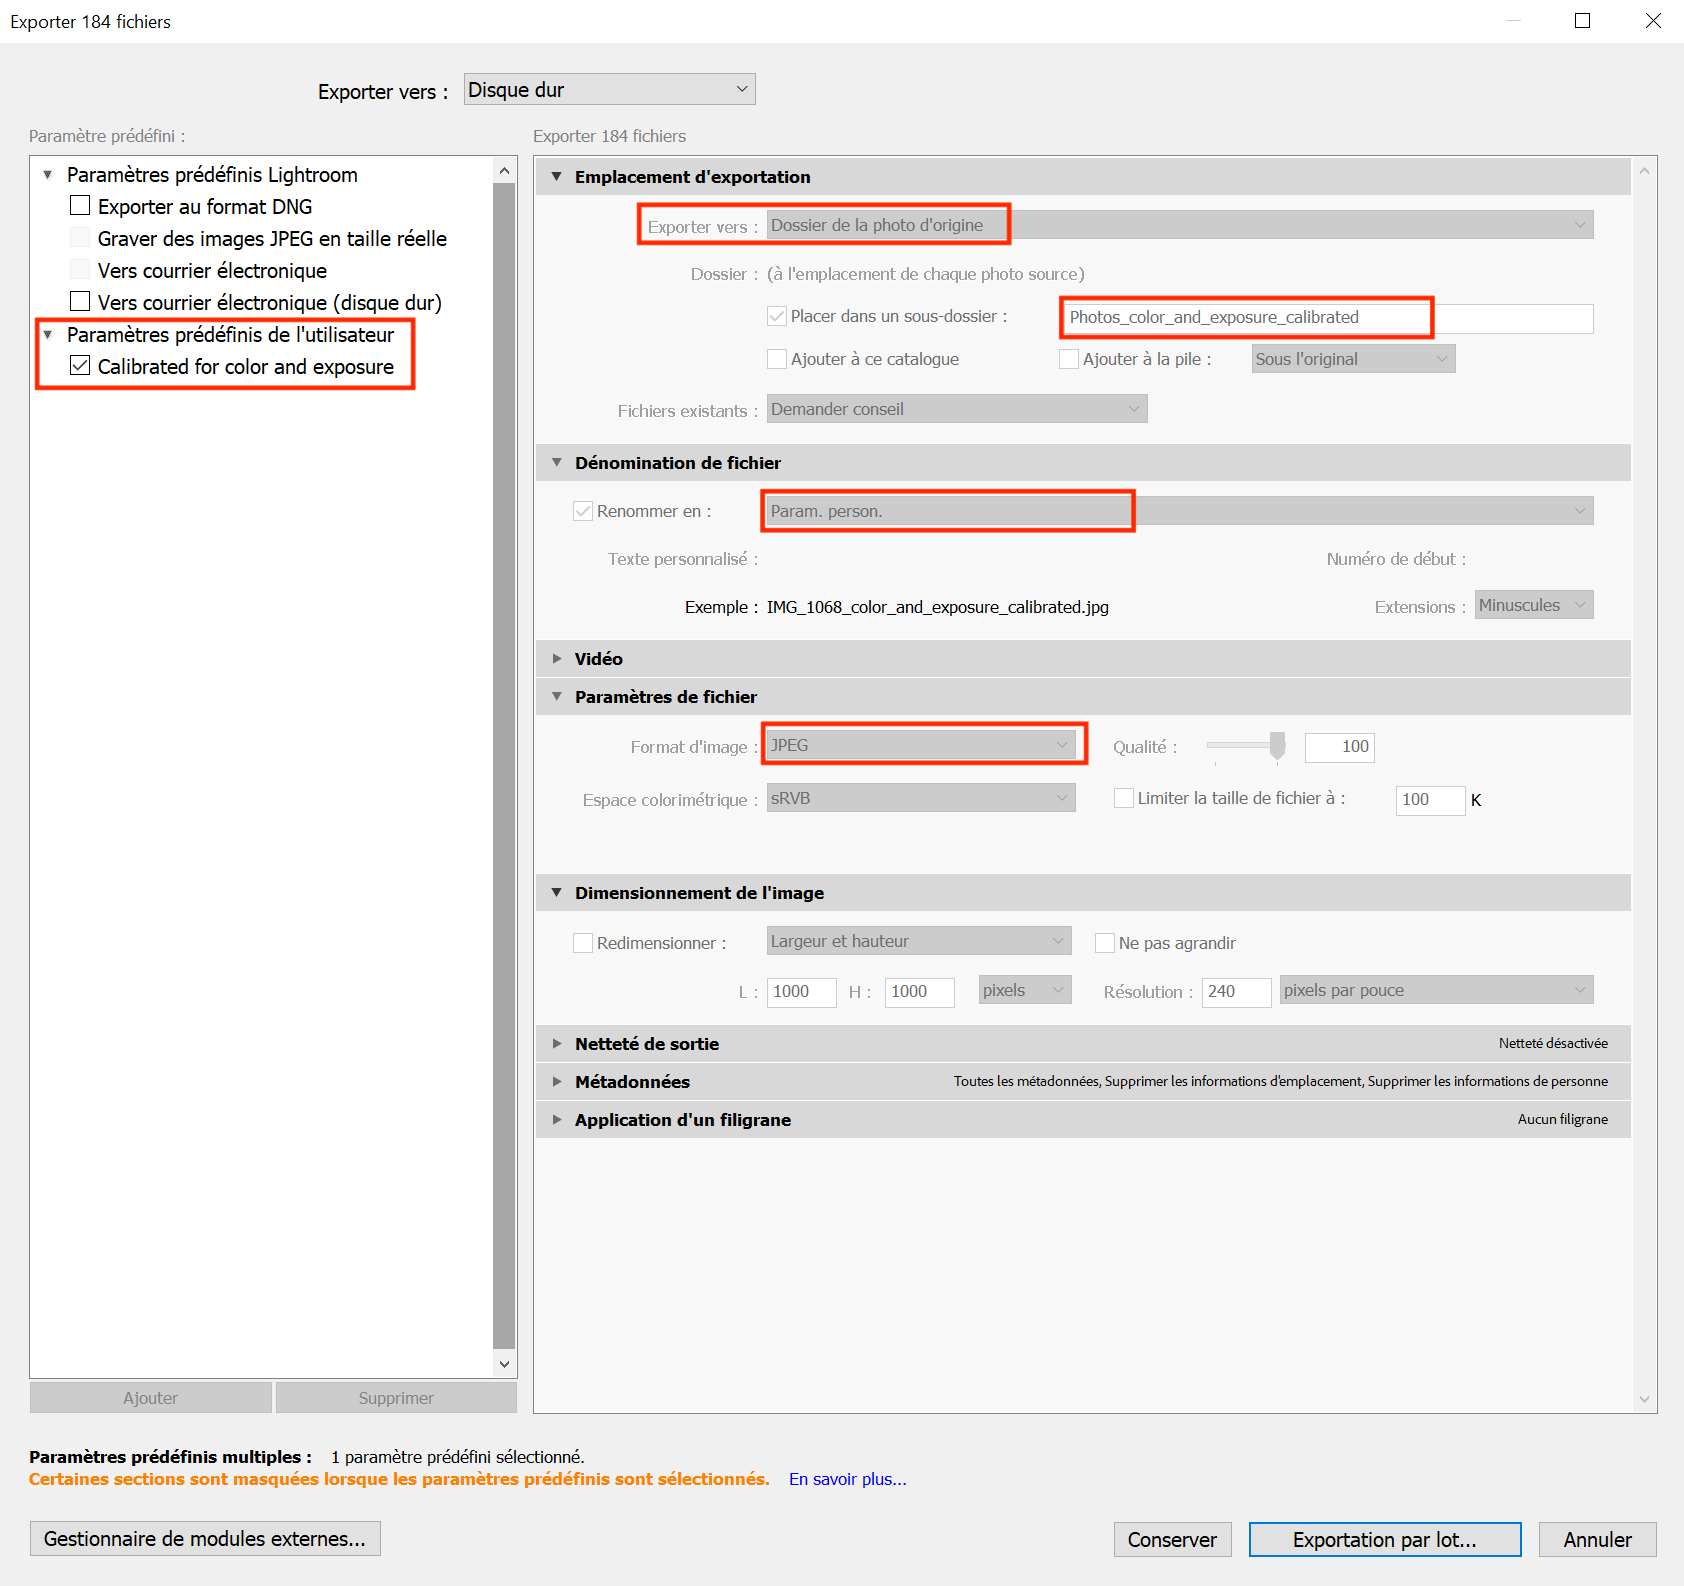
\includegraphics[width=0.9\textwidth,height=\textheight]{Figures/export_capture_1.png}
\caption{You can export using your own personalized parameters and then export
in batch your selection in a specific folder within your folder of
uncalibrated photos for easy access. This method can thus work for any
folder of uncalibrated
photos.}\label{export_parameters}
}
\end{figure}

\hypertarget{blocks}{%
\chapter{Blocks}\label{blocks}}

\hypertarget{equations}{%
\section{Equations}\label{equations}}

Here is an equation.

\begin{equation} 
  f\left(k\right) = \binom{n}{k} p^k\left(1-p\right)^{n-k}
  \label{eq:binom}
\end{equation}

You may refer to using \texttt{\textbackslash{}@ref(eq:binom)}, like see Equation \eqref{eq:binom}.

\hypertarget{theorems-and-proofs}{%
\section{Theorems and proofs}\label{theorems-and-proofs}}

Labeled theorems can be referenced in text using \texttt{\textbackslash{}@ref(thm:tri)}, for example, check out this smart theorem \ref{thm:tri}.

\begin{theorem}
\protect\hypertarget{thm:tri}{}\label{thm:tri}For a right triangle, if \(c\) denotes the \emph{length} of the hypotenuse
and \(a\) and \(b\) denote the lengths of the \textbf{other} two sides, we have
\[a^2 + b^2 = c^2\]
\end{theorem}

Read more here \url{https://bookdown.org/yihui/bookdown/markdown-extensions-by-bookdown.html}.

\hypertarget{callout-blocks}{%
\section{Callout blocks}\label{callout-blocks}}

The R Markdown Cookbook provides more help on how to use custom blocks to design your own callouts: \url{https://bookdown.org/yihui/rmarkdown-cookbook/custom-blocks.html}

\hypertarget{d-model-reconstruction-in-agisoft-metashape}{%
\chapter{3D model reconstruction in Agisoft Metashape}\label{d-model-reconstruction-in-agisoft-metashape}}

\hypertarget{download-agisoft-metashape}{%
\section{Download Agisoft Metashape}\label{download-agisoft-metashape}}

Download the Agisoft Metashape professional edition software
\href{https://www.agisoft.com/downloads/installer/}{here}. Make sure that
your computer fills the \href{https://www.agisoft.com/downloads/system-requirements/}{minimum system
requirements}.
The standard edition doesn't allow the use of the scale option that we
will need to add a scale on our models.

\begin{figure}
\centering

\includegraphics[width=0.2\textwidth,height=\textheight]{Figures/logo_metashape.jpeg}
\caption{Agisoft Metashape}
\end{figure}

\hypertarget{initial-tweaks}{%
\section{Initial tweaks}\label{initial-tweaks}}

Agisoft Metashape can use graphic cards at certain steps of the model
construction such as image matching and depth maps calculation. To
enable the use of the graphic hardware (GPU):

\begin{itemize}
\item
  Select Preferences command from the Tools menu.
\item
  In Preferences dialog select GPU tab.
\item
  Select available GPU devices in GPU tab of the Preferences window
\end{itemize}

This step has to be done only once.

This protocol has been elaborated using the version 1.7.1 of Agisoft
Metashape. The latest version of Metashape is now version 1.8.2, but we
still made the following changes. In order to obtain accurate thin
structures, such as petal margin, and avoid holes in your mesh in
Agisoft Metashape 1.5.x or later (up to our knowlege) you will need to
activate ONCE the \emph{Visibility consistent mesh} function in \emph{Tools \textgreater{}
Preferences \textgreater{} Advanced \textgreater Tweaks}, then \emph{Add} and fill in \emph{Parameters}
with \emph{BuildModel/tvl1\_mesh} and select the value as \emph{False} (figure
\protect\hyperlink{metashape_tweaks}{\[metashape_tweaks\]}). Additionally, to use the anterior
version of the depth maps generation process, add ONCE the tweak :
\emph{BuildDepthMaps/pm\_enable} and set the value to \emph{False} (figure
\protect\hyperlink{metashape_tweaks}{\[metashape_tweaks\]}).

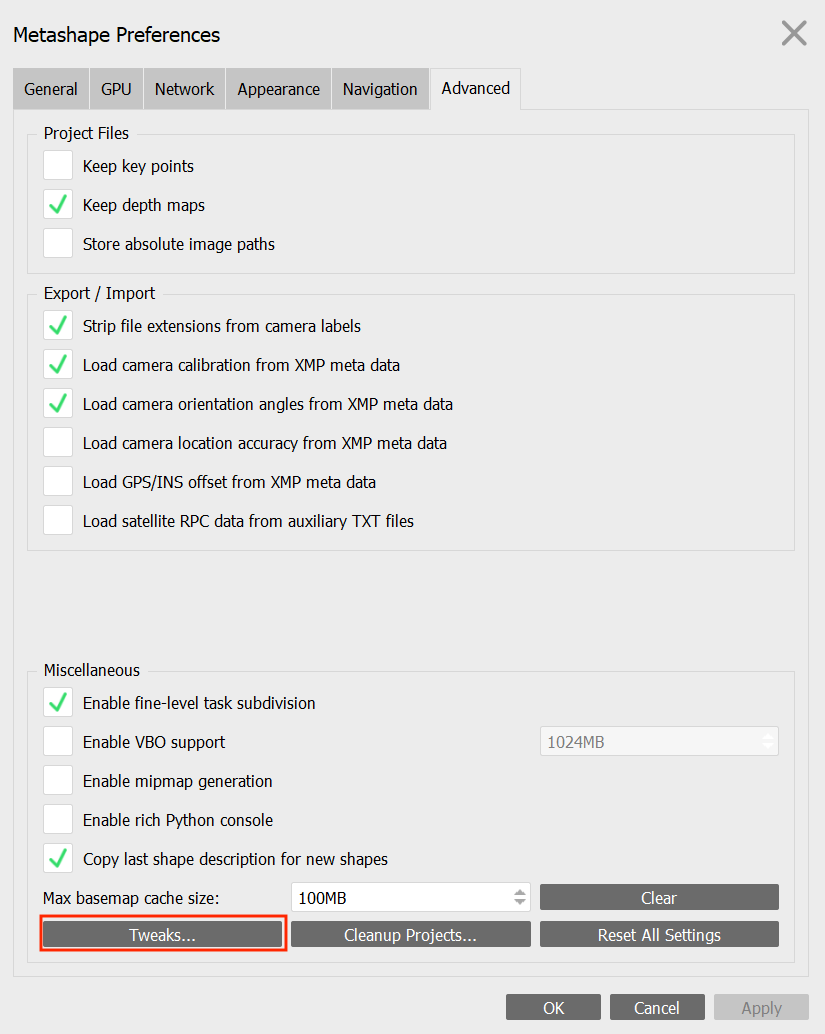
\includegraphics[width=1\textwidth,height=\textheight]{Figures/Metashape_tweaks_1.png}

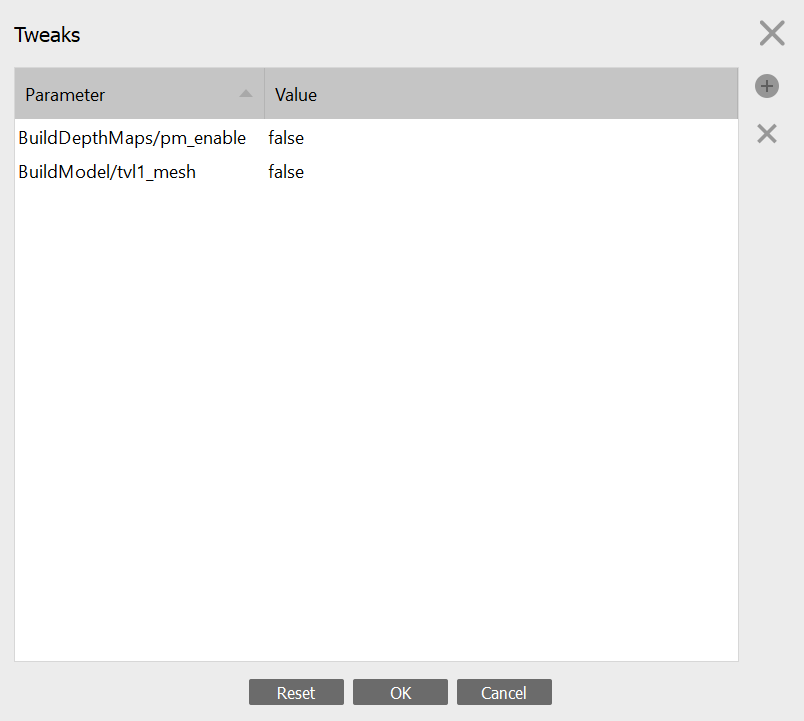
\includegraphics[width=1\textwidth,height=\textheight]{Figures/Metashape_tweaks_2.png}

\hypertarget{overview-of-the-model-building-pipeline}{%
\section{Overview of the model building pipeline}\label{overview-of-the-model-building-pipeline}}

To build a model, we need to do the following steps: 1) Import the
calibrated photos, 2) apply masks to remove background on the photos, 3)
align the cameras, 4) calculate depth maps, 5) build the 3D model
(mesh), and 6) reconstruct the final texture (model color). There could
be different approaches for each of the steps and options will be given
below.

One important note is whether all the pictures (cameras) are aligned
simultaneously of if it is necessary to proceed by groups of pictures
that correspond to each flower positions. The first approach is quicker
and normally results in more accurate models. However, it does not work
all the times. We recommend to try it first and if it fails to use the
alternative approach, which is to divide the pictures in different
"chunks" that will create partial 3D models.

\hypertarget{photo-importation}{%
\section{Photo importation}\label{photo-importation}}

Go to \emph{Workflow}, click on \emph{Add Photos}, and click \emph{Open}. Once the
photos are imported, they are in a single "chunk", which is a group of
photos.

To try to align all the photos simultaneously (ideal approach), you need
to arrange them in "camera groups", where each camera group contains
all pictures taken with the same flower orientation. Once this is done,
you can add the first photo of each set of photos representing the
label, and right click on this photo and select \emph{disable cameras}. This
allows you to not take it into account while reconstructing the model,
but to keep all the information about the flower in your Metashape
project.

\hypertarget{mask-application}{%
\section{Mask application}\label{mask-application}}

Masks represent selected areas that are excluded from the feature
detection procedure when applied to key points detection. When several
keypoints are detected as the same point (matched as projections of the
same 3D point on different photos), then it is considered as a tie
point. If masks are applied to tie points, then if a key point is masked
in at least one image, it will not be considered. You can thus use a
single or just a few masks with the second method (apply masks to tie
points). It is however possible to automatically apply masks on each
photo to better constrain key point detection (apply masks to
keypoints). Using masks helps in removing points to be detected in the
background during image alignment procedure. You can see examples
\href{https://agisoft.freshdesk.com/support/solutions/articles/31000158967-aligning-turntable-photos-with-background-suppression-from-single-mask-in-agisoft-metashape}{here}
on the Agisoft helpdesk portal.

\textbf{Step-by-step mask application workflow}

\begin{enumerate}
\def\labelenumi{\arabic{enumi}.}
\item
  Duplicate one of your photos, and fill it in black in any image
  manipulation software, and rename it as \emph{background.jpg}. You can
  also take a picture of the lightbox without your flower just before
  starting to shoot and use this image as background. This sometimes
  work better.
\item
  Right click on a photo in one of your chunk in your Metashape
  project.
\item
  Click on \emph{Masks}, \emph{Import Masks} and in the box that appears select
  method "From Background", operation \emph{Replacement}.
\item
  Enter the same name as the name of your background you just saved.
\item
  Depending on the flower, the value for \emph{Tolerance} can vary between
  approximately 40 and 60. For some pale flowers you may need a lower
  tolerance value (e.g.~30).
\item
  Test different values of tolerance on a single photo first, but when
  you have a value that is satisfactory (that create a masks with the
  border of the flower well defined) you can select \emph{Apply to entire
  workspace}
\item
  Click OK
\item
  This will automatically produce masks around the flowers for all the
  photos in all your chunks. This is why we need a contrasting white
  background behind the flower.
\item
  Check for masks that need touch ups (next section).
\end{enumerate}

\begin{figure}
\centering
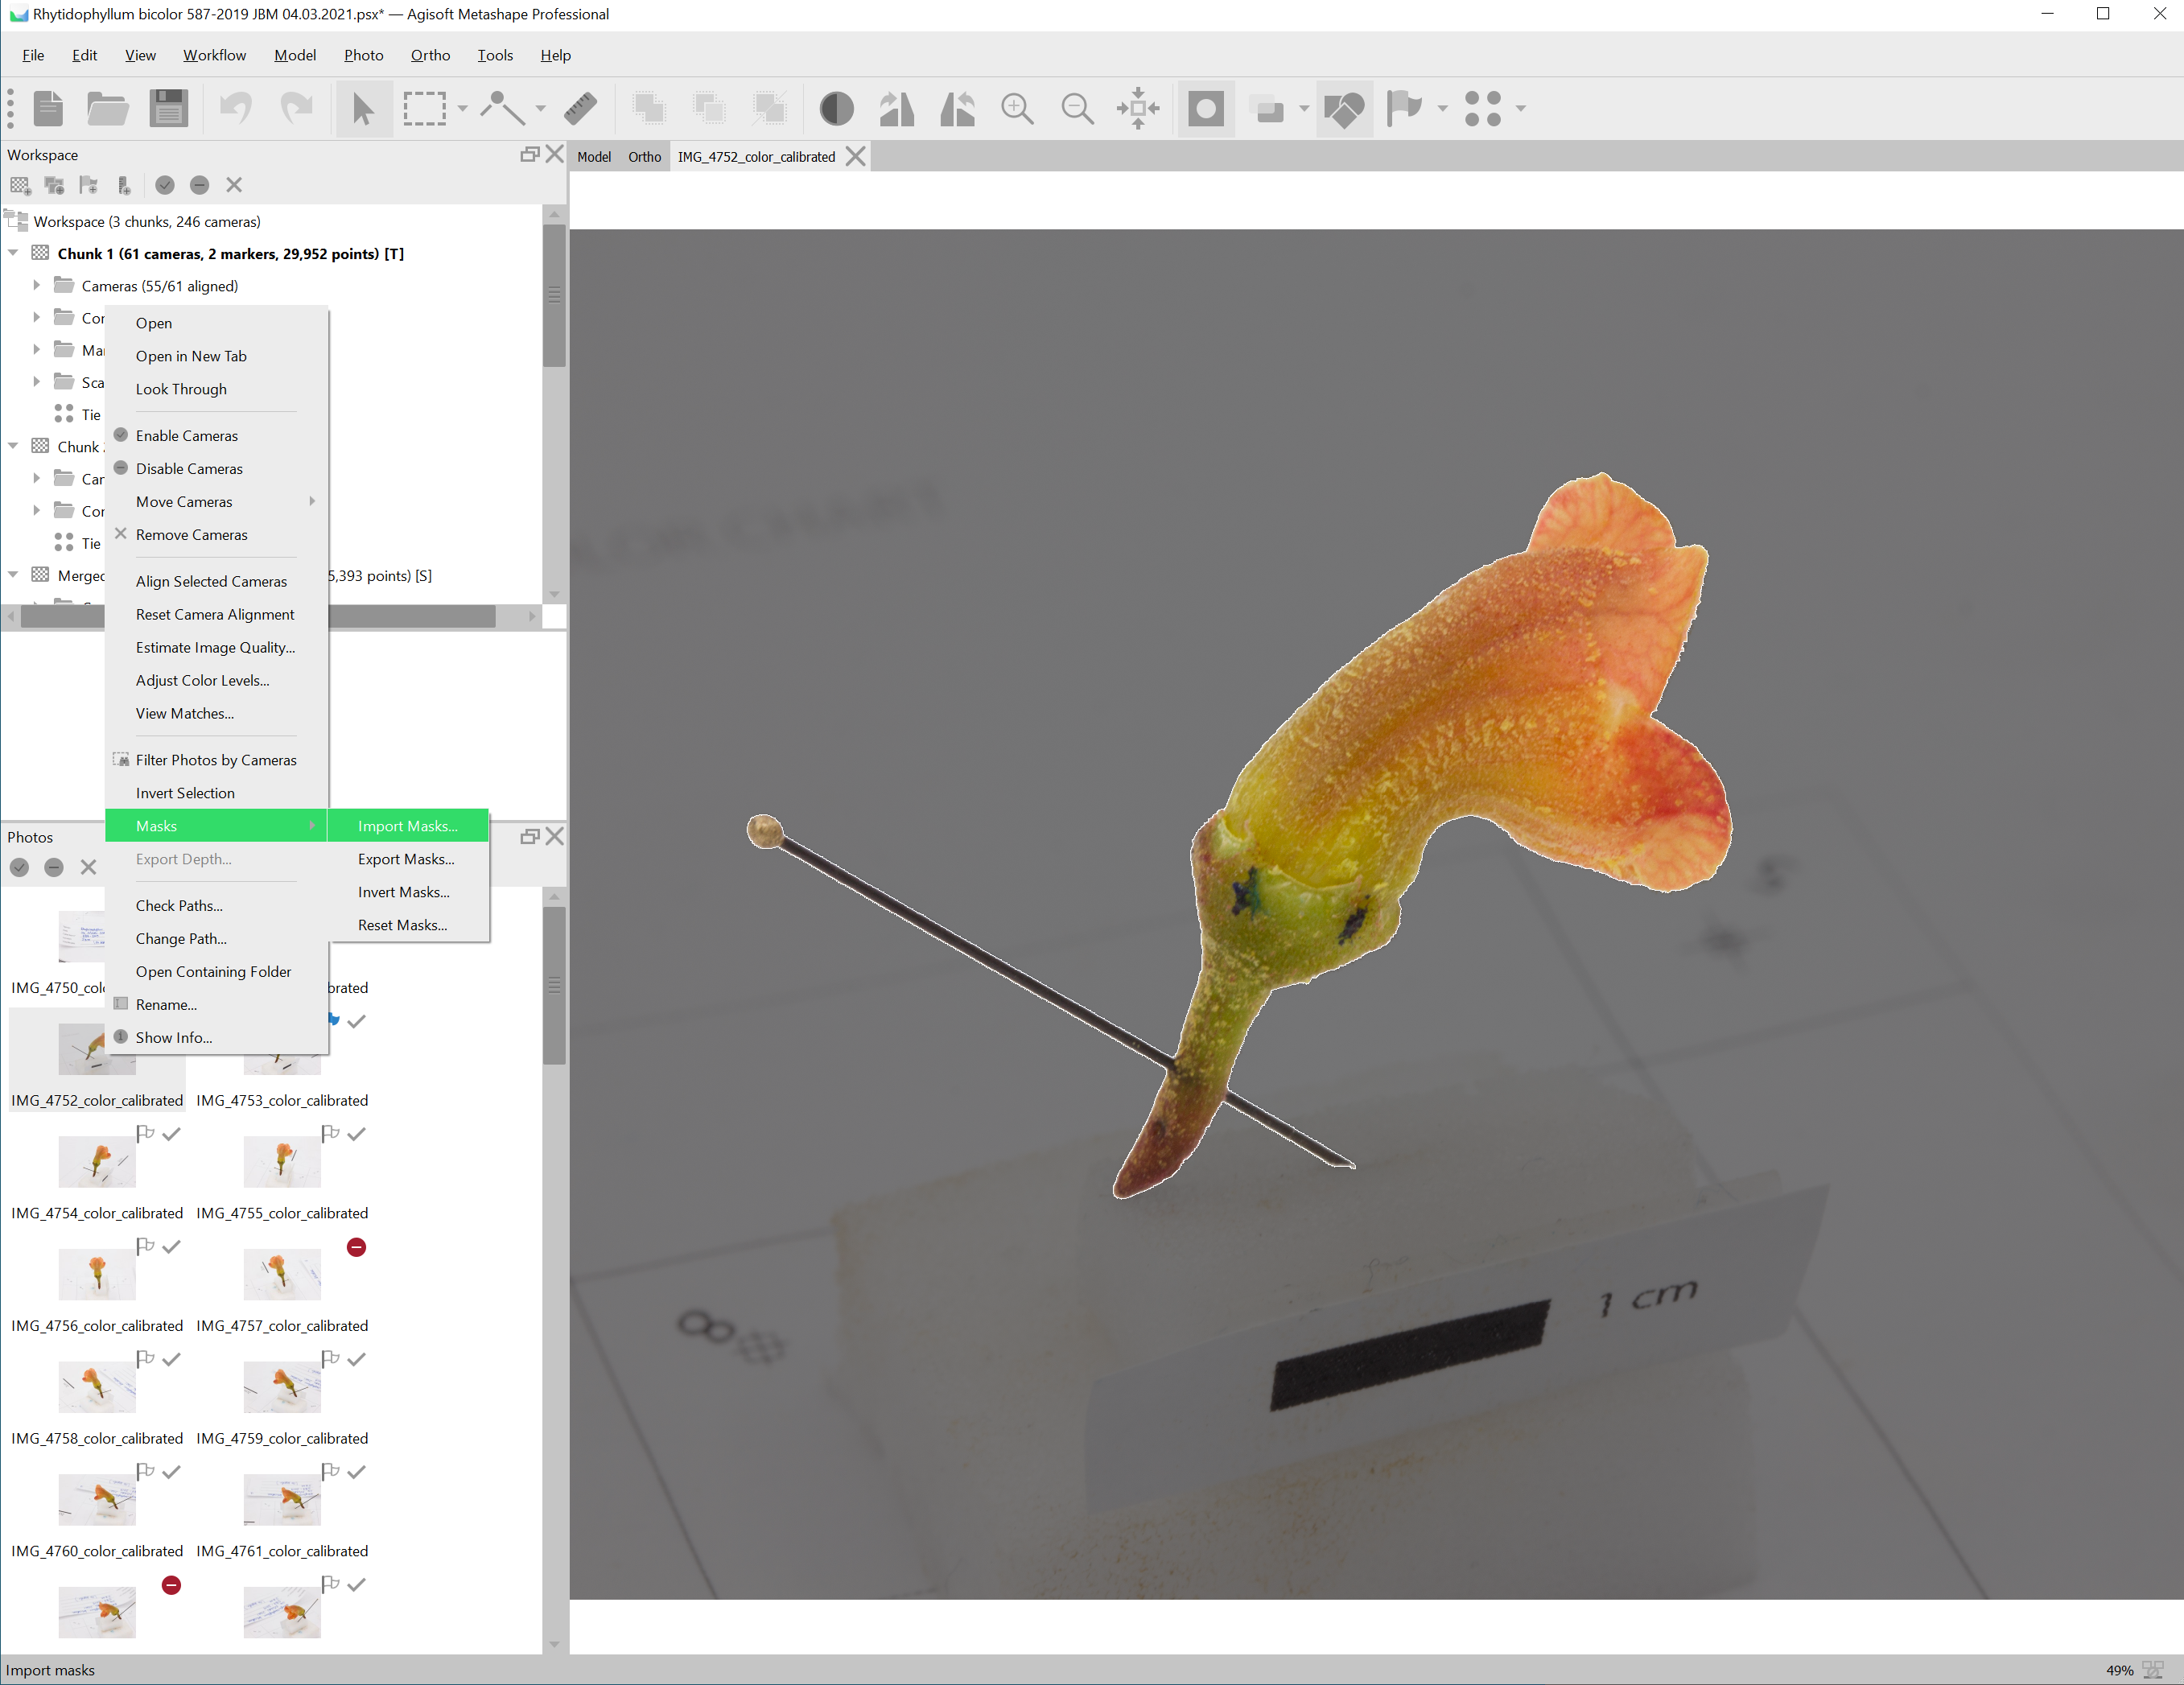
\includegraphics[width=1\textwidth,height=\textheight]{Figures/Metashape_mask_right_click.png}
\caption{Right click on an image to select a mask to
import.}
\end{figure}

\begin{figure}
\centering
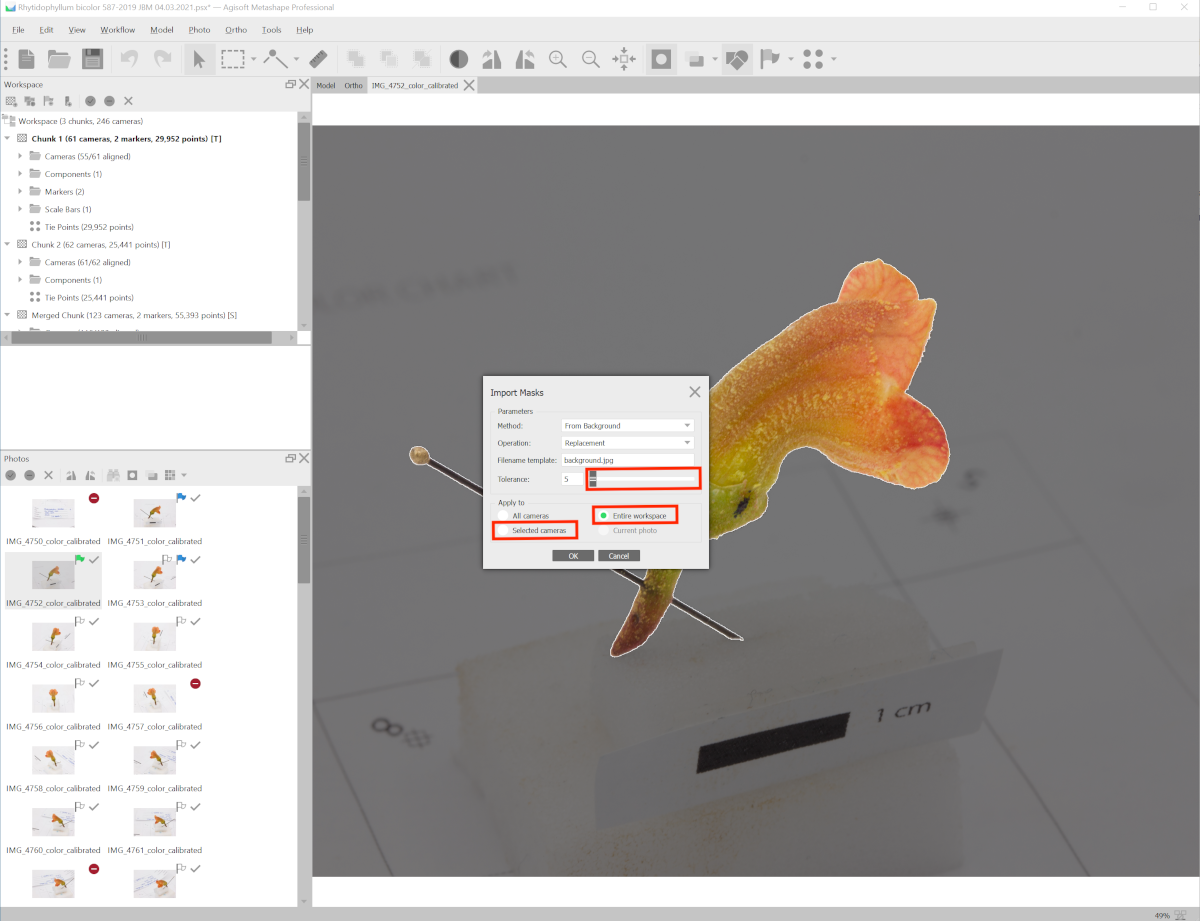
\includegraphics[width=1\textwidth,height=\textheight]{Figures/Metashape_masks_tolerance.png}
\caption{Import mask from a black image \emph{background.jpg}, and select a
tolerance value, to test on the selected camera (the image you
right-clicked on). If the automatic mask is automatically well adjusted
around the flower shape (darker gray around the flower), then apply to
entire workspace (all the
images).}
\end{figure}

\textbf{Alternative masking method using Adobe Photoshop} It is also possible
to use Adobe Photoshop to apply masks. We did not find particular
improvements compared to the Agisoft Metashape approach.

\begin{enumerate}
\def\labelenumi{\arabic{enumi}.}
\item
  Go to the file containing the pictures of chunk 1. Copy and paste
  this file, naming it accordingly (e.g.~\emph{Chunk1-Background}).
\item
  Go to Adobe Photoshop version 19.1 and up.
\item
  Make a copy of all of the photos you'll be using and place them in a
  new folder labeled \emph{Chunk1-masks}.
\item
  Then, you will need to create ONCE a Photoshop action, that will be
  subsequently reused (see figures below) :

  \begin{figure}
  \centering
  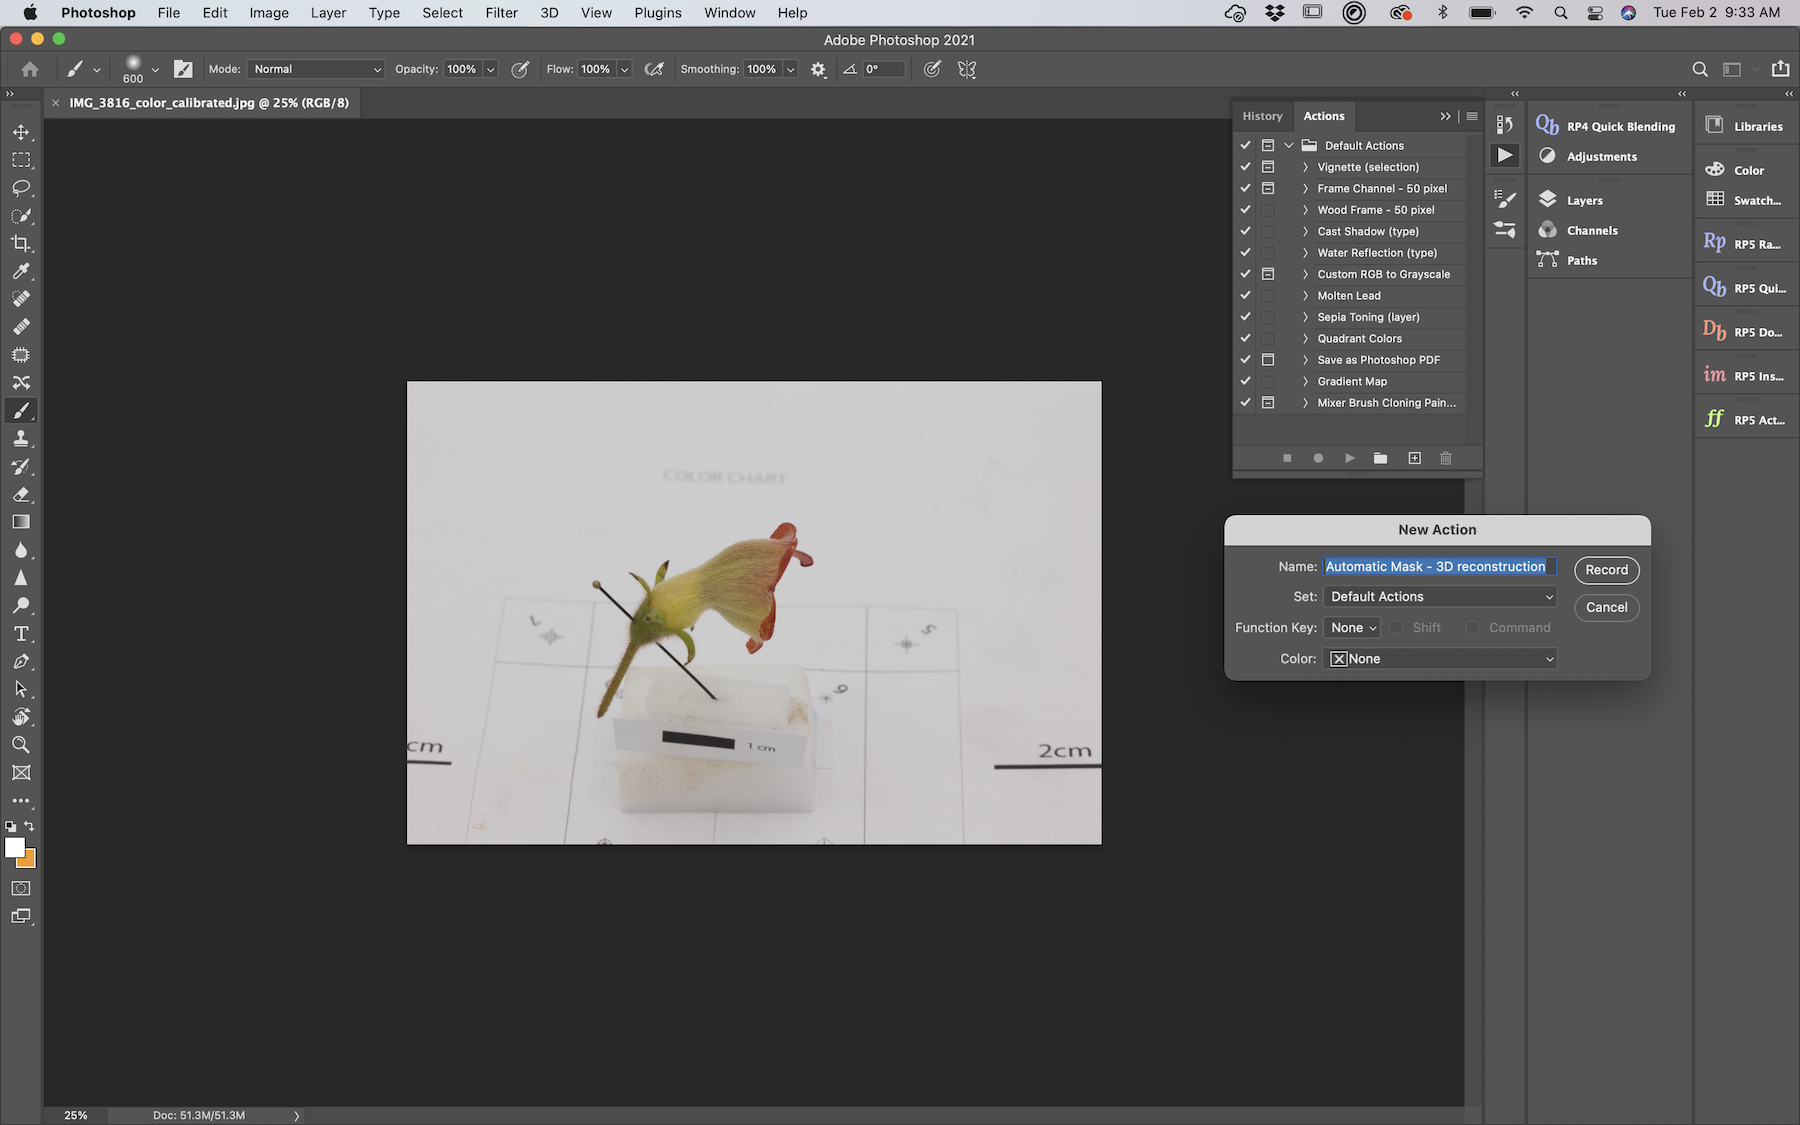
\includegraphics{Figures/mask_1.png}
  \caption{Record a new action called \emph{Automatic Mask - 3D
  reconstruction}}
  \end{figure}

  \begin{figure}
  \centering
  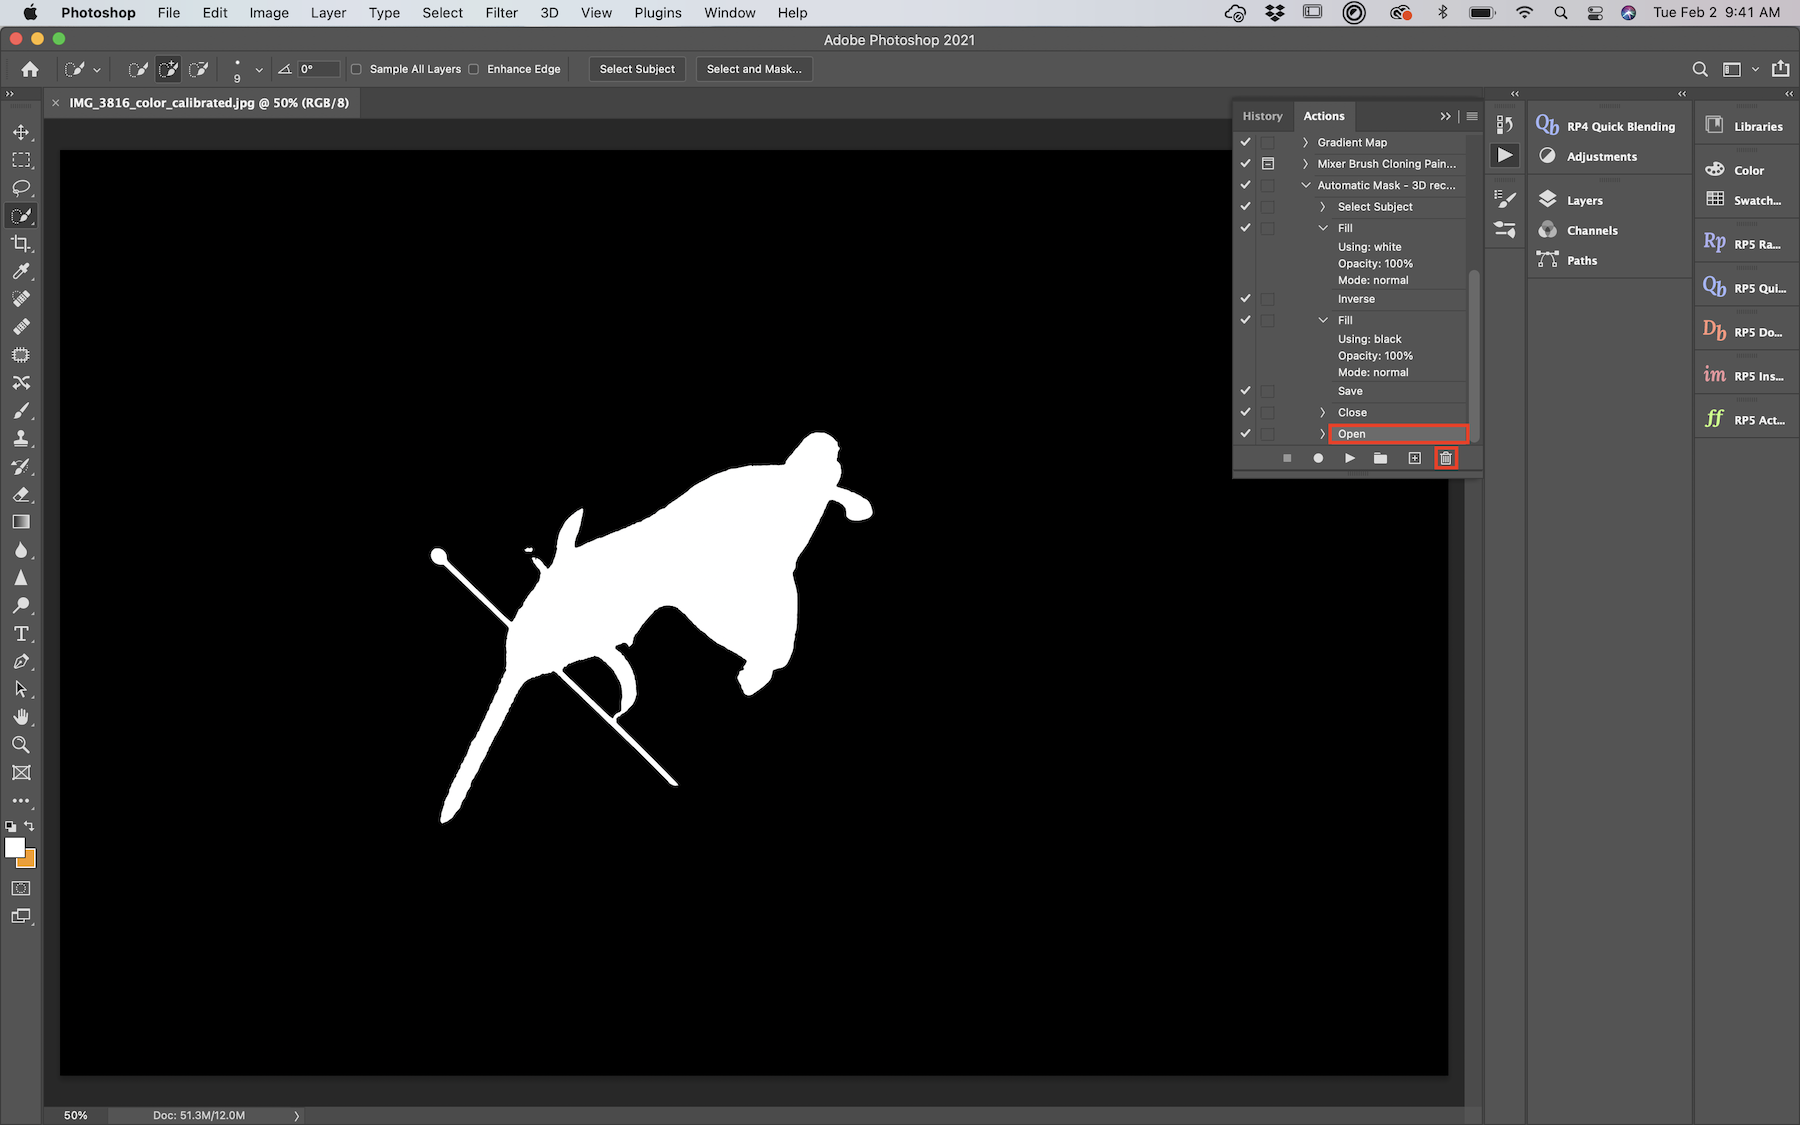
\includegraphics{Figures/mask_2.png}
  \caption{When you reopen your photo, don't forget to remove this extra task
  in your action.}
  \end{figure}

  \begin{figure}
  \centering
  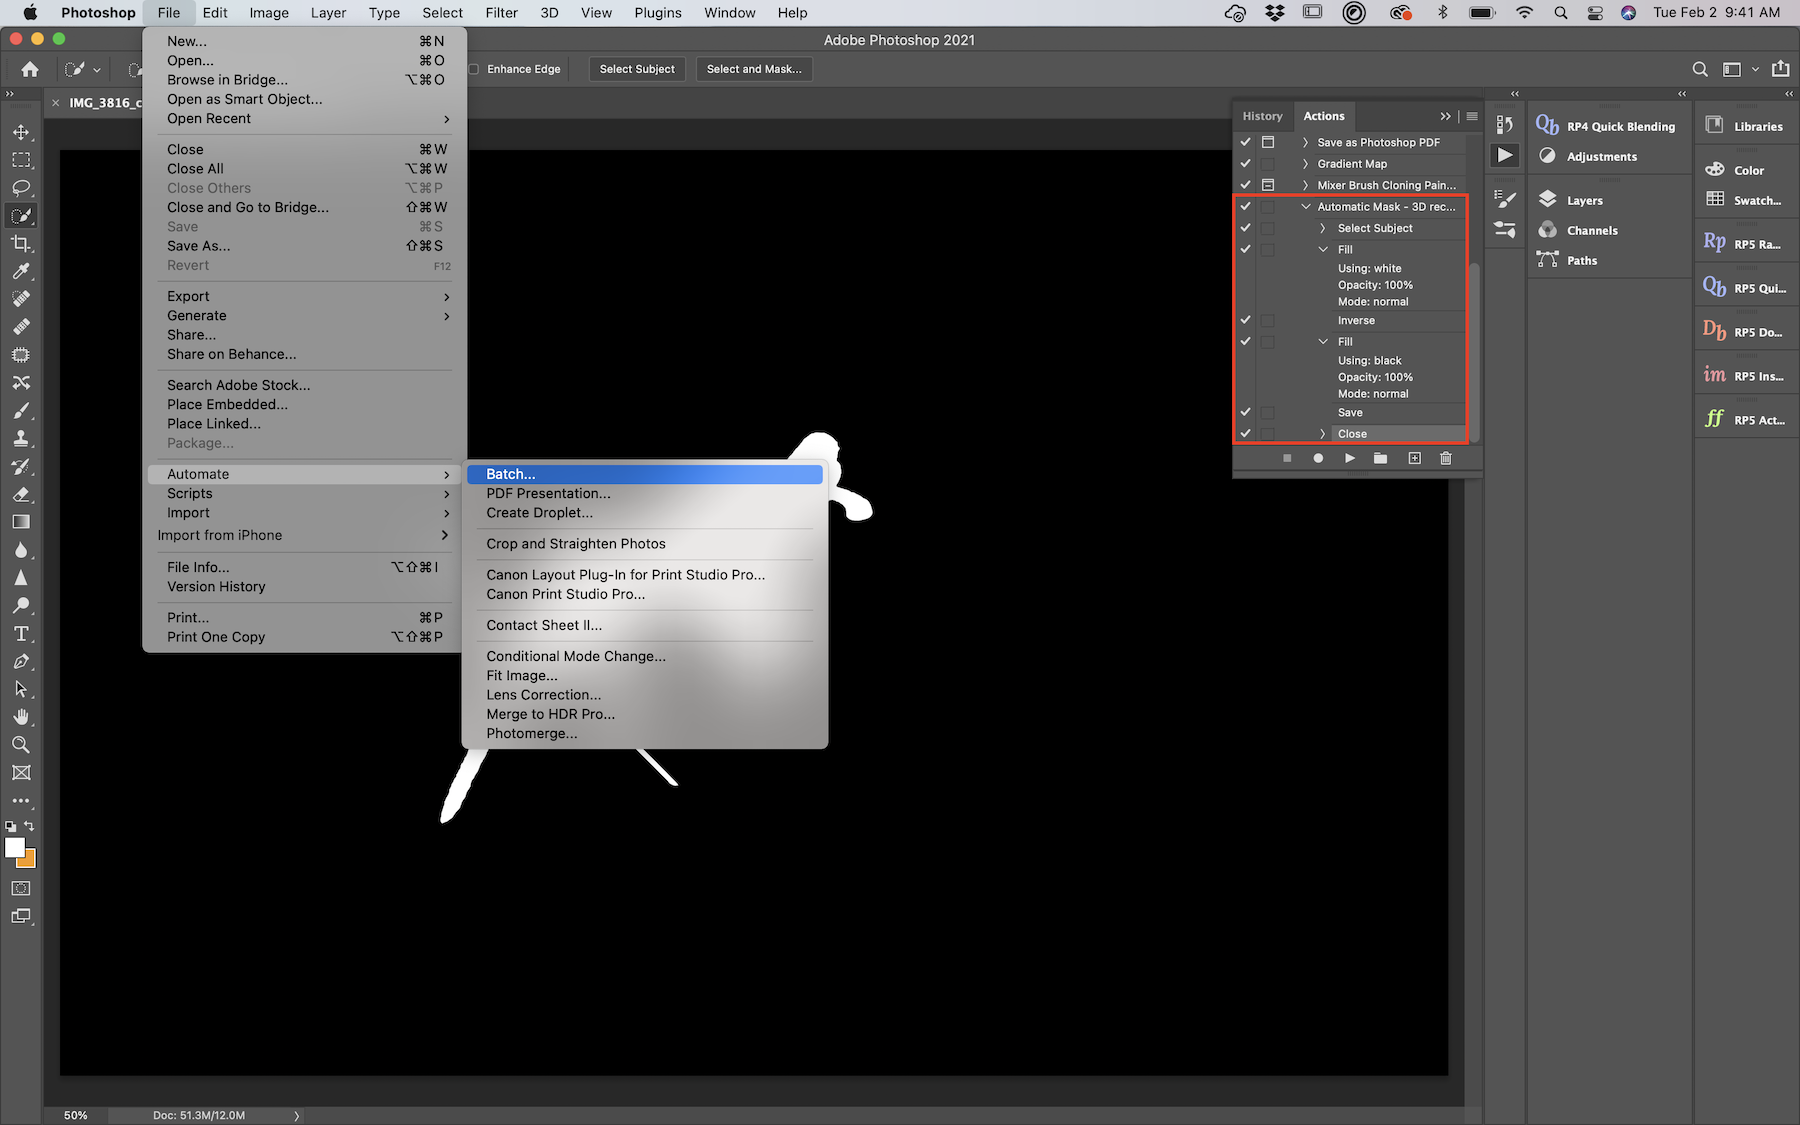
\includegraphics{Figures/mask_3.png}
  \caption{The action should include \emph{Select Subject, Fill, Inverse, Fill,
  Save, Close}, and you can batch process this action to a specific
  folder of copied photos to create
  masks.}
  \end{figure}

  \begin{figure}
  \centering
  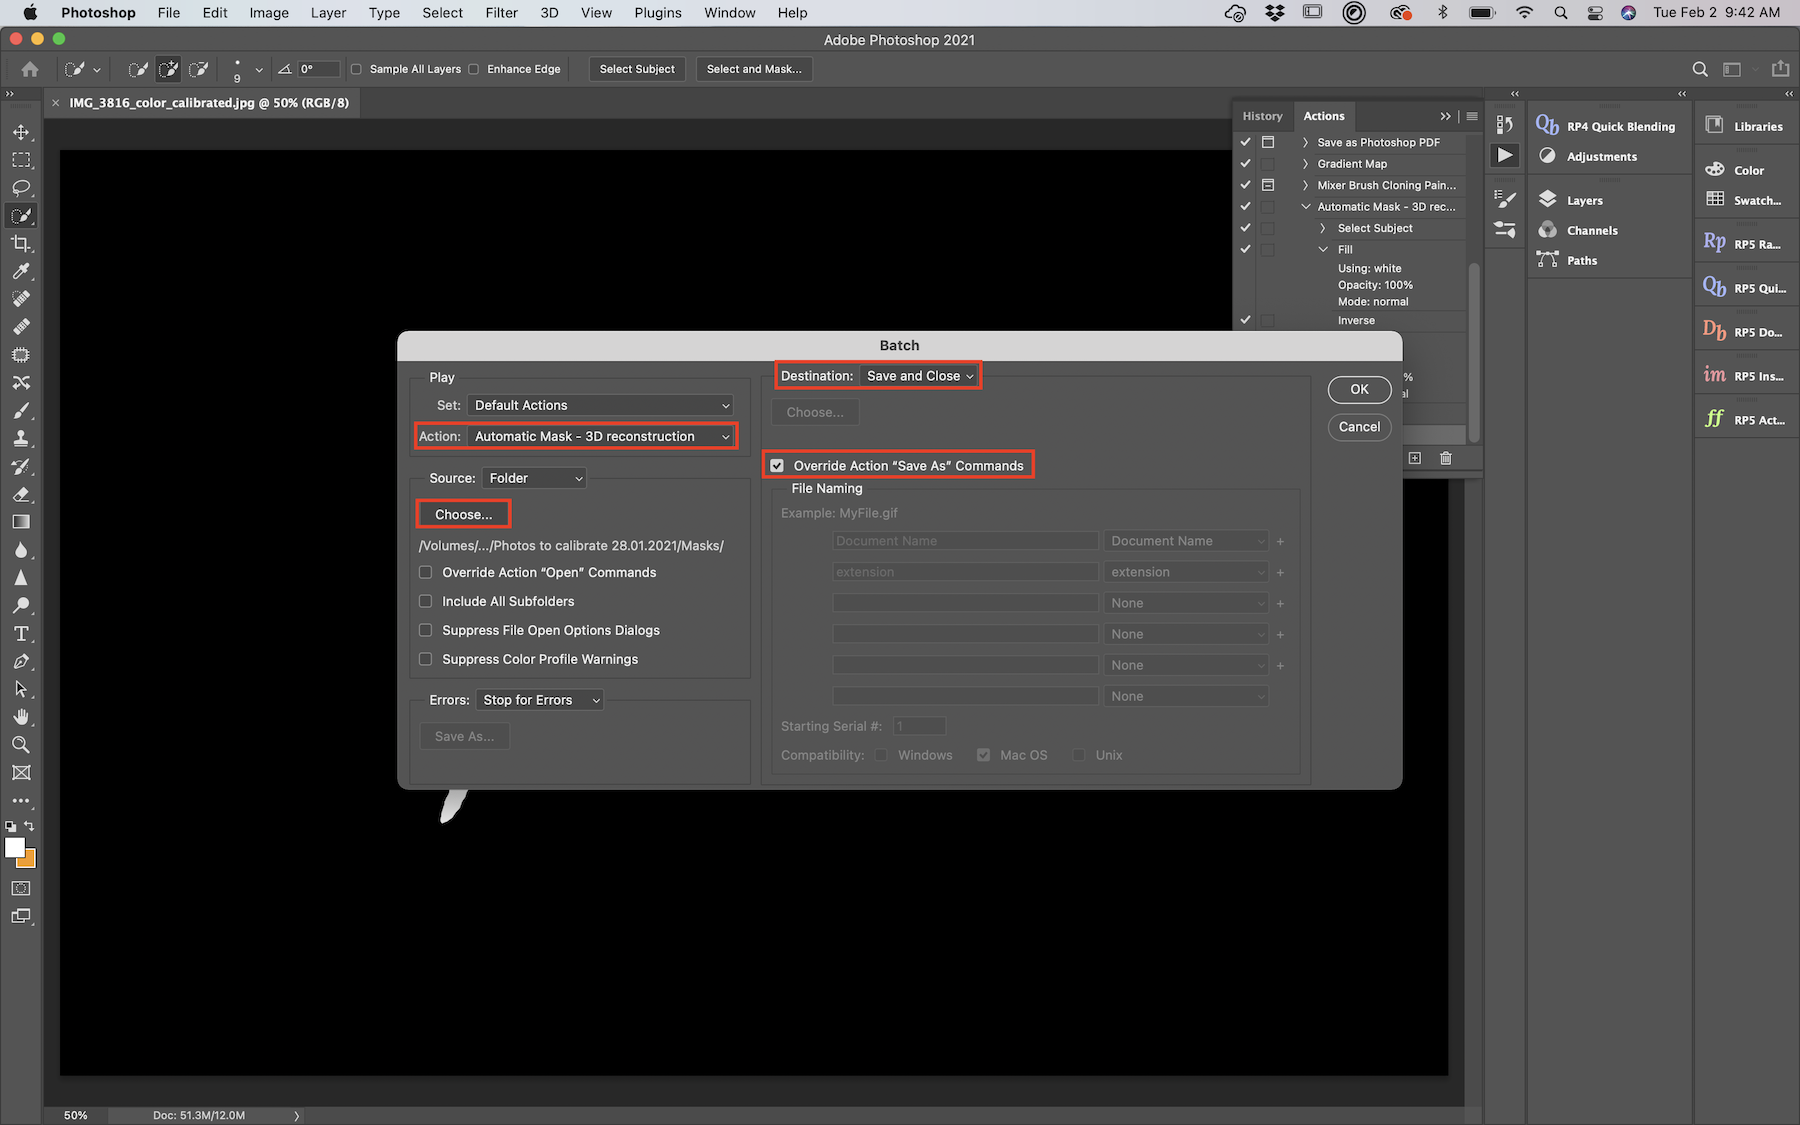
\includegraphics{Figures/mask_4.png}
  \caption{Apply the action to the folder of copied photos called
  \emph{Chunk1-masks}.}
  \end{figure}
\item
  Now you should have tranformed all your copied photos into masks,
  with the foreground object in white, and the background in black.
\item
  Go to Agisoft Metashape and right click on the first camera (photo)
  of chunk 1. Click on \emph{Masks \textgreater{} Import Masks} and in the box that
  appears select method \emph{From file}, operation \emph{Replacement}. In
  \emph{Filename Template} use \emph{filename.jpg}. Select \emph{Apply to all
  cameras} and then click \emph{OK}.
\item
  Check the masks for touch ups.
\end{enumerate}

\hypertarget{masks-touch-ups}{%
\section{Masks touch ups}\label{masks-touch-ups}}

The automatic application of masks at the previous steps is sometimes
not entirely satisfactory for all photos. It is possible to add or
remove parts of masks using the selection tool and the add/remove/invert
buttons (Figure \protect\hyperlink{tools_masks}{25}). You can then use the selection tools to
select areas that are not the flower and add the selection to the mask
(Figure \protect\hyperlink{tools_masks}{25}). You also remove the scale and the
entomological pin at this step. Additionally, you can invert the
selection, or remove the selected areas from the mask with the icons on
the right hand side of the add to mask icon.

\begin{figure}
\hypertarget{tools_masks}{%
\centering
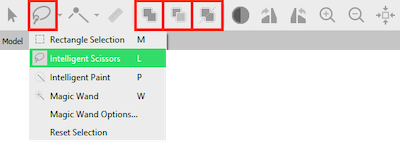
\includegraphics[width=0.5\textwidth,height=\textheight]{Figures/tools_masks.png}
\caption{Selection tools and add selection to mask
tool}\label{tools_masks}
}
\end{figure}

\hypertarget{camera-alignment}{%
\section{Camera alignment}\label{camera-alignment}}

\begin{enumerate}
\def\labelenumi{\arabic{enumi}.}
\item
  Click on the chunk you want to align, which could comprise several
  camera groups.
\item
  Make sure to disable photos you don't want (the label photo, and
  blurry photos) and that the masks are clean.
\item
  Go to \emph{Workflow}, \emph{Align Photos} and put the accuracy on \emph{High} or
  \emph{Very high}. In the section \emph{Advanced}, check \emph{Generic
  pre-selection}, and select \emph{Apply masks} to \emph{key points}, and click
  \emph{OK}. Note that if you have applied the masks to only some photos,
  select \emph{Apply masks} to \emph{tie points}.
\item
  If you are aligning several chunks of photos, it is possible to run
  this job in batch for each chunk in \emph{workflow} \textgreater{} \emph{batch process} \textgreater{}
  \emph{Add} button \textgreater{} select the \emph{job type} as \emph{Align photos} to apply to
  \emph{all chunks} or select specific ones \textgreater{} add parameters listed above
  (Figure \protect\hyperlink{batch_alignment}{26}).

  \begin{figure}
  \hypertarget{batch_alignment}{%
  \centering
  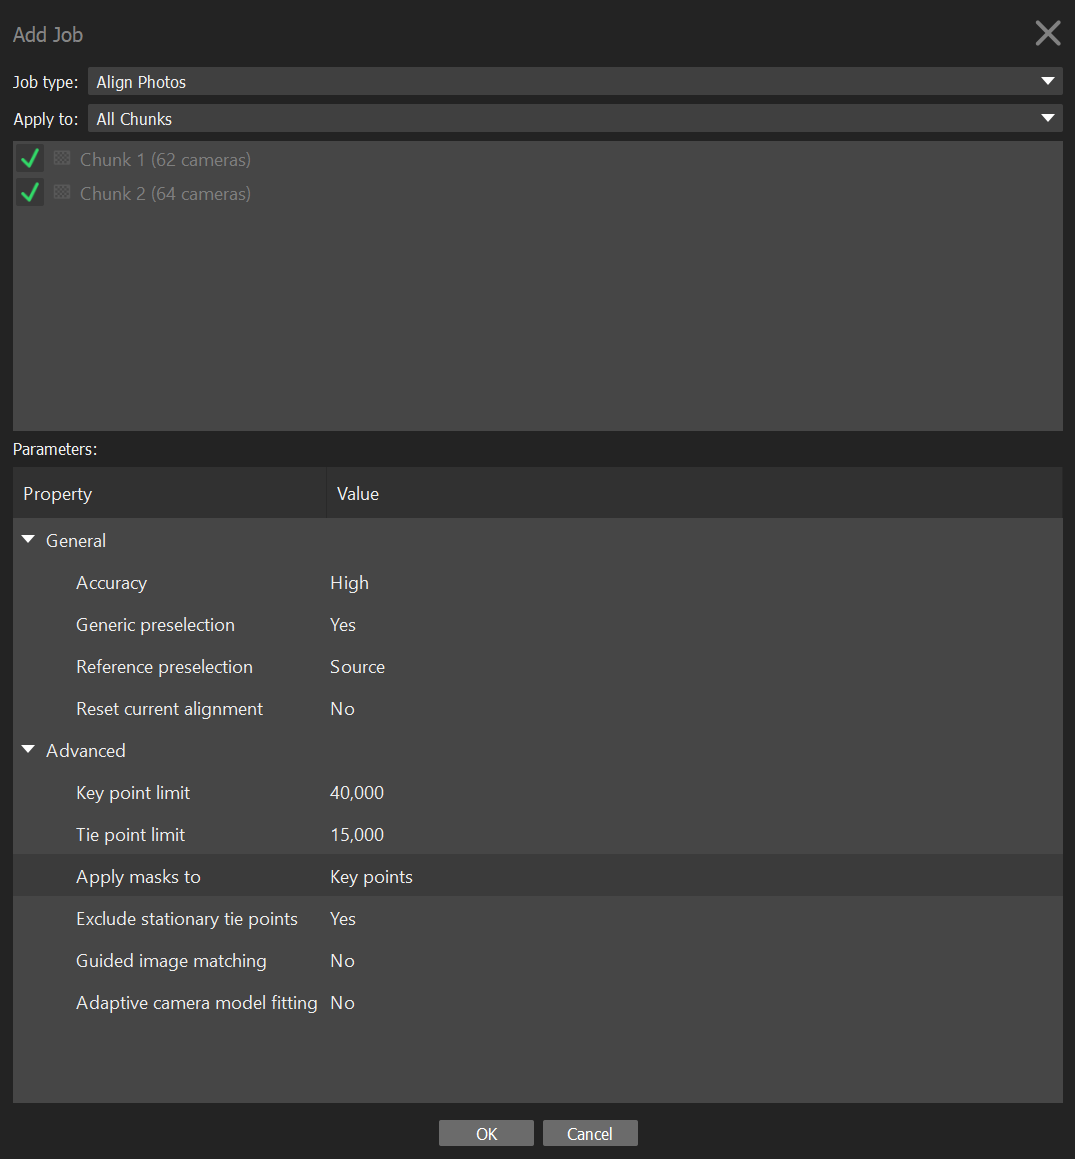
\includegraphics[width=0.5\textwidth,height=\textheight]{Figures/metashape_batch_align.png}
  \caption{Align photos in multiple
  chunks}\label{batch_alignment}
  }
  \end{figure}
\item
  \textbf{Optional: align using markers} If the different camera cannot
  align properly, it is possible to place homologous markers on the
  flower, defined as remarkable points on the flower (distinguishable
  pattern such as color dots on the corolla, for example), or by
  little pen marks at the surface of the flower when homologous
  markers lacks. These points need to be clearly identifiable on all
  camera groups. You will need at least 5 markers per flower, ideally
  positioned in different regions of the flower (e.g., near the
  peduncle, sepals tips, petals). Do not use points from the
  background to align chunks as it is independent from the flower (the
  flower changes position relative to the background).

  \begin{enumerate}
  \def\labelenumii{\arabic{enumii}.}
  \item
    Right click on the picture
  \item
    Then click on \emph{Place Marker} \textgreater{} \emph{New Marker}.
  \item
    In the left panel, rename them accordingly. Make sure to use the
    same nomenclature on each chunk to be able to merge them
    according to their names.
  \end{enumerate}
\item
  To help the software recognize the markers, spread the manual
  markers on photos throughout the chunk (It is normally sufficient to
  place it on 2-3 photos and the software normally places them
  properly on the others, but make sure the markers are all properly
  placed).
\item
  Repeat the step for each marker and each chunk.
\item
  Select one chunk. Go to \emph{Workflow \textgreater{} Align Chunks}, select the
  chunks you want to align, set the method as \emph{Markers based} and then
  click \emph{OK}. Repeat for all chunks to align.
\item
  \textbf{Optional} If the camera alignment is not satisfactory, it is
  possible to clean the tie point obtained and try to realign the
  cameras. For instance, on the tie point generated by the alignment,
  you can delete outlier and imprecise points (Figure
  \protect\hyperlink{removing_points}{\[removing_points\]}):

  \begin{enumerate}
  \def\labelenumii{\arabic{enumii}.}
  \item
    In the top menu, click on \emph{Model} and then \emph{Gradual Selection}.
    Select \emph{Reconstruction uncertainty} on \emph{Criterion} and play with
    the \emph{Level} value to remove the uncertain points. The higher the
    value, the worst is the point placed. Values between 30 and 10
    generally give good results. Then \emph{OK}. Press \emph{Delete} on your
    keyboard to delete the selected points in red. You don't need
    much more than 10,000 points for good photo alignments.
  \item
    After removing uncertain points, go to the \emph{Reference} panel and
    click on \emph{Optimize Camera} to optimize camera position. Select
    all of the cameras.
  \item
    In \emph{Model \textgreater{} Gradual Selection}, ensure that \emph{Reprojection
    error} parameter is below 1. If it is not, check if the
    alignment runs well (camera needs to form a full circle above
    the object). If the alignment fails, try to re-align photos by
    following step 3 (don't forget to check the box "reset current
    alignment"). If the alignment didn't fail, go to \emph{Model \textgreater{}
    Gradual Selection \textgreater{} Reproduction error}, and set the level to 1
    and click OK. Then press \emph{Delete}.
  \item
    Manually remove remaining outliers using the selection tool.
  \end{enumerate}
\item
  Repeat these steps for each chunk.
\end{enumerate}

\begin{figure}
\hypertarget{model_orientation1}{%
\centering
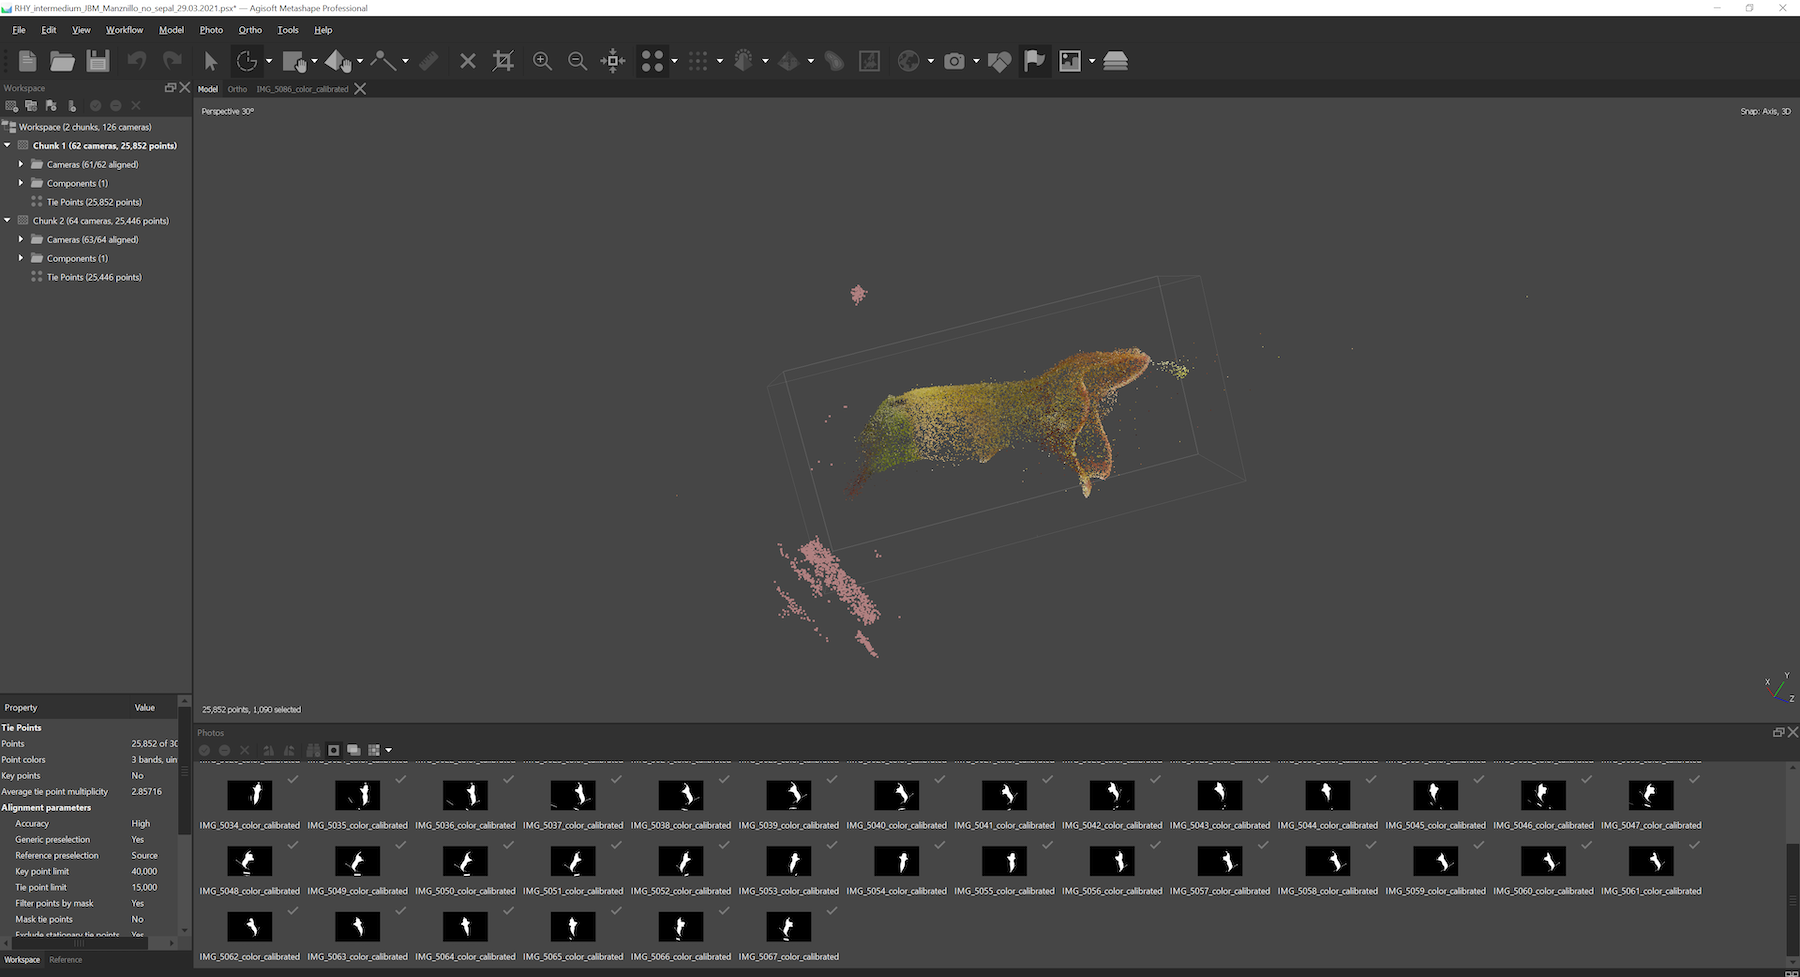
\includegraphics[width=1\textwidth,height=\textheight]{Figures/metashape_delete_selectedpoints.png}
\caption{Use the selection tool to remove background
points}\label{model_orientation1}
}
\end{figure}

\begin{figure}
\hypertarget{model_orientation2}{%
\centering
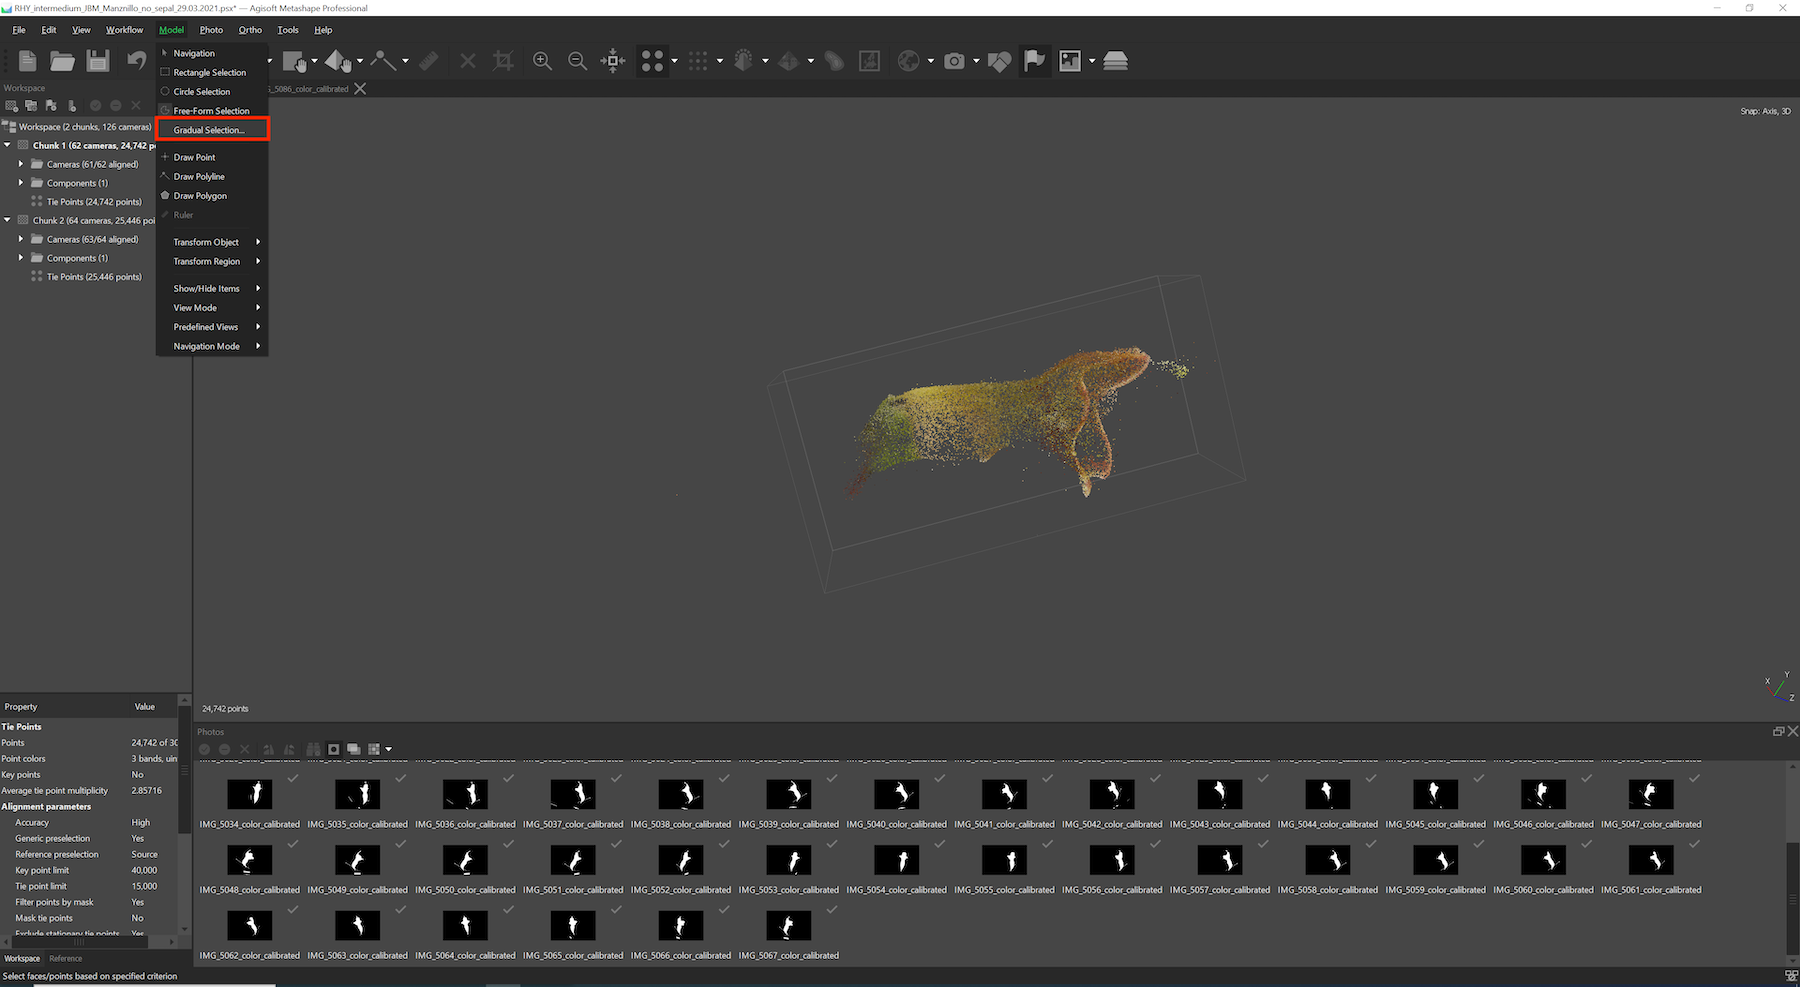
\includegraphics[width=1\textwidth,height=\textheight]{Figures/metashape_gradual_selection.png}
\caption{Use the gradual selection tool to remove additional mis-calculated
points}\label{model_orientation2}
}
\end{figure}

\textbf{Note: If the alignment fails using only one chunk and two or more
camera groups, then it will be necessary to divide your job in several
chunks. Each chunk should then contain photos from one flower position.
Once the chunks are ready, you can proceed with the alignment following
the previous steps.}

\hypertarget{align-chunks-together}{%
\section{Align chunks together}\label{align-chunks-together}}

\textbf{Note: This step is only necessary if your project is divided in
several chunks.}

At this step, it is important to align the different chunks with each
other before they can be combined in a complete model. There are two
ways to do this. The approach using tie points is quick but does not
work all the time. If it fails, you will have to use the approach using
markers.

To align using tie points :

\begin{enumerate}
\def\labelenumi{\arabic{enumi}.}
\item
  Select the chunks to align together.
\item
  Go to \emph{Workflow} \textgreater{} \emph{Align Chunks}, select the chunks you want to
  align together, set the method as \emph{Point based} (Figure
  \protect\hyperlink{Align_chunk}{29}).
\item
  Restrict the key points with masks.
\item
  Click on \emph{OK}.
\end{enumerate}

To align using markers :

\begin{enumerate}
\def\labelenumi{\arabic{enumi}.}
\item
  Place homologous markers on the flower, defined as remarkable points
  on the flower (distinguishable pattern such as color dots on the
  corolla, for example), or by little pen marks at the surface of the
  flower when homologous markers lacks. These points need to be
  clearly identifiable on all chunks. You will need at least 5 markers
  per flower, ideally positioned in different regions of the flower
  (e.g., near the peduncle, sepals tips, petals). Do not use points
  from the background to align chunks as it is independent from the
  flower (the flower changes position relative to the background).

  \begin{enumerate}
  \def\labelenumii{\arabic{enumii}.}
  \item
    Right click on the picture
  \item
    Then click on \emph{Place Marker} \textgreater{} \emph{New Marker}.
  \item
    In the left panel, rename them accordingly. Make sure to use the
    same nomenclature on each chunk to be able to merge them
    according to their names.
  \end{enumerate}
\item
  To help the software recognize the markers, spread the manual
  markers on photos throughout the chunk (It is normally sufficient to
  place it on 2-3 photos and the software normally places them
  properly on the others, but make sure the markers are all properly
  placed).
\item
  Repeat the step for each marker and each chunk.
\item
  Select one chunk. Go to \emph{Workflow \textgreater{} Align Chunks}, select the
  chunks you want to align, set the method as \emph{Markers based} and then
  click \emph{OK}. Repeat for all chunks to align.
\end{enumerate}

When the chunks are aligned, a \[T\] is put at the end of your chunk
name to notify that it is transformed. You can check the alignment using
the icon to show aligned chunks (icon of layers on top of each others,
Figure \protect\hyperlink{show_aligned_chunk}{30}). The different chunks should be well
aligned over the whole flower. If the alignment of your chunks is
unsatisfactory, try to place more markers on recognizable features and
spread across the whole flower. Additionally, you can manually align
chunks using the tools to move the models in the space, but this is
highly not recommended.

\begin{figure}
\hypertarget{Align_chunk}{%
\centering
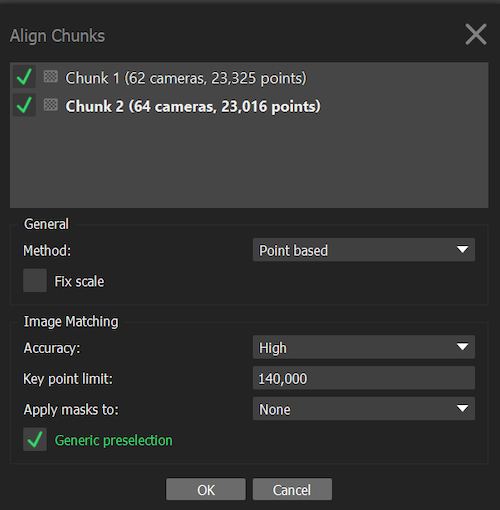
\includegraphics[width=1\textwidth,height=\textheight]{Figures/metashape_align_chunks.png}
\caption{Align chunks}\label{Align_chunk}
}
\end{figure}

\begin{figure}
\hypertarget{show_aligned_chunk}{%
\centering
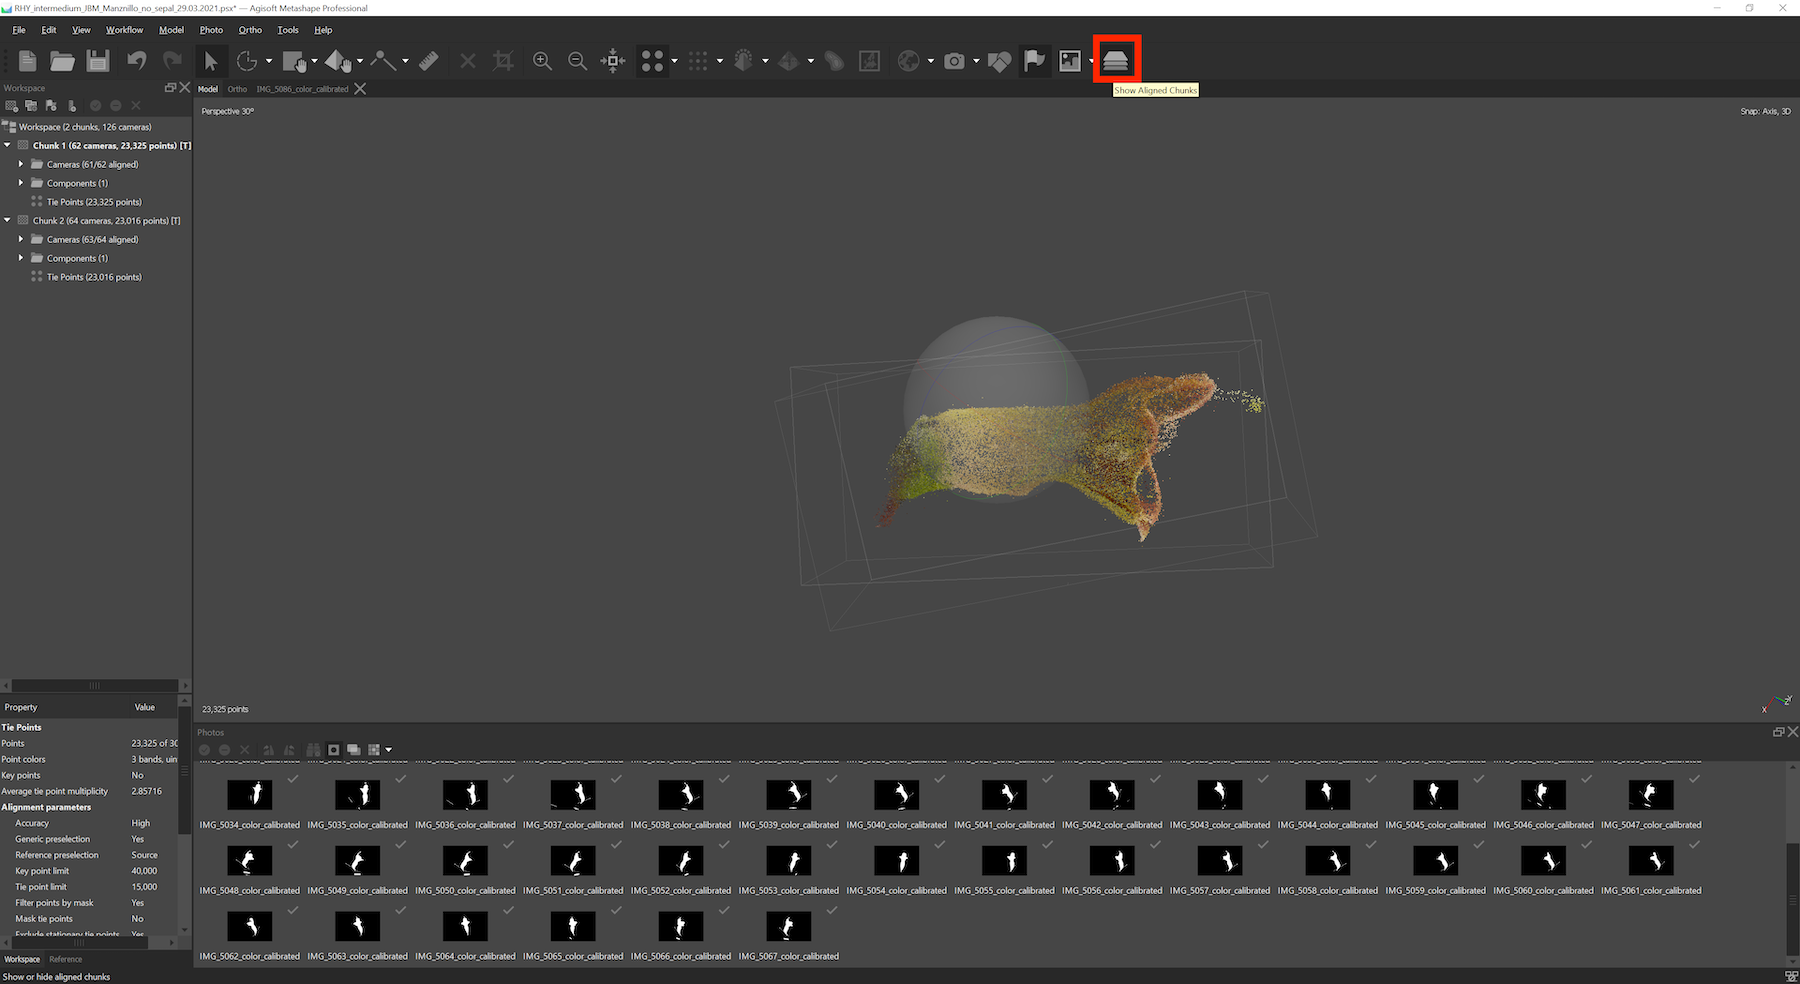
\includegraphics[width=0.9\textwidth,height=\textheight]{Figures/metashape_show_aligned_chunks.png}
\caption{Show aligned chunks to verify their
positions}\label{show_aligned_chunk}
}
\end{figure}

\hypertarget{merge-chunks}{%
\section{Merge chunks}\label{merge-chunks}}

\textbf{Note: This step is only necessary if your project is divided in
several chunks.}

The next step is to merge chunks together when they are well aligned.
Click on \emph{Workflow \textgreater{} Merge chunks}, and merge using either the tie
point method or the markers method depending on the option selected
above.

\hypertarget{build-3d-mesh}{%
\section{Build 3D mesh}\label{build-3d-mesh}}

\begin{enumerate}
\def\labelenumi{\arabic{enumi}.}
\item
  Select the chunk or the merged chunks for which you want to build a
  3D mesh (model).
\item
  Go to \emph{Workflow \textgreater{} Build Mesh}.
\item
  In the dialog box, make sure that \emph{Source Data} is on \emph{Depth maps},
  \emph{Quality} and \emph{Face Count} on \emph{High} (Figure
  \protect\hyperlink{fig:3d_mesh}{31}).
  Note that although it is also possible to generate a mesh from a
  dense point cloud (which has to be built separately), the depth maps
  provide better results for objects with a high number of minor
  details.
\item
  Then go to \emph{Advanced}, check \emph{Calculate vertex colors}. Click OK.
\item
  Once the mesh is produced, you should remove the pin and extra
  floating background parts using the selection tool. This will
  highlight the selection in red.
\item
  Verify your selection and press delete to remove them.
\end{enumerate}

\begin{figure}
\hypertarget{fig:3d_mesh}{%
\centering
\includegraphics[width=0.5\textwidth,height=\textheight]{Figures/metashape_build_mesh.png}
\caption{Build 3D mesh}\label{fig:3d_mesh}
}
\end{figure}

Our protocol merges the chunks to build a tie point model of all chunks
before constructing a model for the merge chunk. We found that this is
the best approach, although it is also possible to build models for each
chunk separately and then merge these models to obtain a full model.

\hypertarget{d-mesh-touch-ups}{%
\section{3D mesh touch ups}\label{d-mesh-touch-ups}}

\begin{enumerate}
\def\labelenumi{\arabic{enumi}.}
\item
  You can smooth the mesh by clicking on \emph{Tools}, \emph{Mesh}, \emph{Smooth
  Mesh}. You can also duplicate a 3D model to save one intact, and
  right click on it, and un-check \emph{Use as default} to keep it as an
  archived model. If you smooth a mesh, you can't undo it.
\item
  You can fill holes in your mesh by clicking on \emph{Tools \textgreater{} Mesh \textgreater{}
  Close Holes}. Note that if your holes are too big, the closing
  function can create unwanted structures. Similarly as the smoothing,
  you can't undo closing holes in the mesh. \textbf{HOWEVER}, this will
  remove the vertex colors in version 1.7.2, which we will need to
  place landmarks when doing the morphometrics.
\end{enumerate}

\hypertarget{build-texture}{%
\section{Build texture}\label{build-texture}}

To build the texture : \emph{Workflow \textgreater{} Build Texture}, use the preset
values and click OK.

\hypertarget{scaling}{%
\section{Scaling}\label{scaling}}

To scale the model, go to the pictures of your merged chunk and follow
these steps :

\begin{enumerate}
\def\labelenumi{\arabic{enumi}.}
\item
  On a picture displaying the scale bar, add new markers at each end
  of the scale bar and on a couple of additional photos.
\item
  In the left panel, select both markers and click on the icon \emph{Add
  scale} (Figure \protect\hyperlink{metashape_scale}{32}).
\item
  Go to the \emph{Reference} panel, select the scale and add 0.01 as
  reference.
\item
  Click on the \emph{Update transform} button (rotating arrows). This is an
  important step, because otherwise the scale will not be incorporated
  to your model.
\item
  To verify if the scale is taken into account, you can use the
  measuring tape tool.
\end{enumerate}

\begin{figure}
\hypertarget{metashape_scale}{%
\centering
\includegraphics[width=0.9\textwidth,height=\textheight]{Figures/metashape_add_scale_2.png}
\caption{Add a scale using
landmarks}\label{metashape_scale}
}
\end{figure}

\hypertarget{model-orientation}{%
\section{Model orientation}\label{model-orientation}}

\begin{enumerate}
\def\labelenumi{\arabic{enumi}.}
\item
  In Metashape, be sure that \emph{Show info} in \emph{Model \textgreater{} Show/Hide Items}
  is checked. You should see at the bottom right of the model panel
  the 3D axes.
\item
  Show grid
\item
  Make sure that the scale is the right one, changing it will affect
  the coordinates of the 3D model. You can verify the scale using the
  measuring tool.
\item
  Use the navigation tool to orient these 3D axes.
\item
  Once you orient the 3D axes in the wanted direction, you can then
  use the tool \emph{Rotate Object} to put the object in the wanted
  direction, and at the center of the grid, facing the right side of
  the grid.
\item
  Orient the binding box as well with the cross on the ventral side,
  and the two dash facing the opening of the flower. Note that
  depending on the software you use to open the model, the first view
  orientation may change when you open the final object file.
\end{enumerate}

\includegraphics[width=1\textwidth,height=\textheight]{Figures/metashape_orientation.png}

\includegraphics[width=1\textwidth,height=\textheight]{Figures/metashape_orientation_2.png}

\hypertarget{export-model-and-texture}{%
\section{Export model and texture}\label{export-model-and-texture}}

\begin{enumerate}
\def\labelenumi{\arabic{enumi}.}
\item
  You can export your 3D model by clicking on \emph{File} \textgreater{} \emph{Export} \textgreater{}
  \emph{Export Model}.
\item
  Name your model
\item
  Choose .ply as the extension.
\item
  In the dialog box, tick the \emph{Vertex colors}. This option will allow
  you to get color on the actual 3D model.
\item
  Select \emph{Export texture} as PNG.
\item
  Make sure to export the texture with transparency, by ticking the
  \emph{Write alpha channel} option. The texture is a separate file, with
  detail color information that is wrapped on the model.
\item
  Click on \emph{OK}.
\end{enumerate}

\hypertarget{sharing-your-book}{%
\chapter{Sharing your book}\label{sharing-your-book}}

\hypertarget{publishing}{%
\section{Publishing}\label{publishing}}

HTML books can be published online, see: \url{https://bookdown.org/yihui/bookdown/publishing.html}

\hypertarget{pages}{%
\section{404 pages}\label{pages}}

By default, users will be directed to a 404 page if they try to access a webpage that cannot be found. If you'd like to customize your 404 page instead of using the default, you may add either a \texttt{\_404.Rmd} or \texttt{\_404.md} file to your project root and use code and/or Markdown syntax.

\hypertarget{metadata-for-sharing}{%
\section{Metadata for sharing}\label{metadata-for-sharing}}

Bookdown HTML books will provide HTML metadata for social sharing on platforms like Twitter, Facebook, and LinkedIn, using information you provide in the \texttt{index.Rmd} YAML. To setup, set the \texttt{url} for your book and the path to your \texttt{cover-image} file. Your book's \texttt{title} and \texttt{description} are also used.

This \texttt{gitbook} uses the same social sharing data across all chapters in your book- all links shared will look the same.

Specify your book's source repository on GitHub using the \texttt{edit} key under the configuration options in the \texttt{\_output.yml} file, which allows users to suggest an edit by linking to a chapter's source file.

Read more about the features of this output format here:

\url{https://pkgs.rstudio.com/bookdown/reference/gitbook.html}

Or use:

\begin{Shaded}
\begin{Highlighting}[]
\NormalTok{?bookdown}\SpecialCharTok{::}\NormalTok{gitbook}
\end{Highlighting}
\end{Shaded}


  \bibliography{book.bib,packages.bib}

\end{document}
